\documentclass[pdftex, 12pt, a4paper]{article}


%%%%%%%%%%%%%%%%%%%%%%%  Загрузка пакетов  %%%%%%%%%%%%%%%%%%%%%%%%%%%%%%%%%%
\usepackage[british,russian]{babel} % выбор языка для документа
\usepackage[utf8]{inputenc} % задание utf8 кодировки исходного tex файла

%\usepackage{showkeys} % показывать метки в готовом pdf

\usepackage{etex} % расширение классического tex
% в частности позволяет подгружать гораздо больше пакетов, чем мы и займёмся далее

%\usepackage{mathtext} % русские буквы в формулах? (и без неё работает)
% Например, $x_{\text{один}}$

%\usepackage{cmap} % для поиска русских слов в pdf --- теперь устарело?

\usepackage{verbatim} % для многострочных комментариев
\usepackage{makeidx} % для создания предметных указателей
\usepackage[X2,T2A]{fontenc}
\usepackage{setspace}
\usepackage{amsmath,amsfonts,amssymb,amsthm}
\usepackage{mathrsfs} % sudo yum install texlive-rsfs
\usepackage{dsfont} % sudo yum install texlive-doublestroke
\usepackage{array,multicol,multirow,bigstrut} % sudo yum install texlive-multirow
\usepackage{indentfirst} % установка отступа в первом абзаце главы
\usepackage{bm}
\usepackage{bbm} % шрифт с двойными буквами
\usepackage[perpage]{footmisc}

\usepackage{dcolumn} % центрирование по разделителю для apsrtable

% создание гиперссылок в pdf
\usepackage[pdftex,unicode,colorlinks=true,urlcolor=blue,hyperindex,breaklinks]{hyperref}



\usepackage[backend = biber]{biblatex}
%\addbibresource{sc_biblio.bib}




% свешиваем пунктуацию
% теперь знаки пунктуации могут вылезать за правую границу текста, при этом текст выглядит ровнее
%\usepackage{microtype}     %этот пакет выдаёт фатальную ошибку












\usepackage{textcomp}  %  Чтобы в формулах можно было русские буквы писать через \text{}

% размер листа бумаги
\usepackage[paper=a4paper,top=13.5mm, bottom=13.5mm,left=16.5mm,right=13.5mm,includefoot]{geometry}

\usepackage{xcolor}


\usepackage{float,longtable}
\usepackage{soulutf8}

\usepackage{enumitem} % дополнительные плюшки для списков
%  например \begin{enumerate}[resume] позволяет продолжить нумерацию в новом списке

\usepackage{mathtools}
\usepackage{cancel,xspace} % sudo yum install texlive-cancel

%\usepackage{minted} % display program code with syntax highlighting
% требует установки pygments и python

\usepackage{numprint} % sudo yum install texlive-numprint
\npthousandsep{,}\npthousandthpartsep{}\npdecimalsign{.}

\usepackage{embedfile} % Чтобы код LaTeXа включился как приложение в PDF-файл

\usepackage{subfigure} % для создания нескольких рисунков внутри одного

\usepackage{tikz, pgfplots} % язык для рисования графики из latex'a
\usetikzlibrary{trees} % tikz-прибамбас для рисовки деревьев
\usepackage{tikz-qtree} % альтернативный tikz-прибамбас для рисовки деревьев
\usetikzlibrary{arrows} % tikz-прибамбас для рисовки стрелочек подлиннее




\usepackage{amscd}  %Пакеты для рисования
\usepackage[matrix,arrow,curve]{xy} %комунитативных диаграмм


%%% Работа с картинками
\usepackage{graphicx}  % Для вставки рисунков
\graphicspath{{images/}{images2/}}  % папки с картинками
\setlength\fboxsep{3pt} % Отступ рамки \fbox{} от рисунка
\setlength\fboxrule{1pt} % Толщина линий рамки \fbox{}
\usepackage{wrapfig} % Обтекание рисунков и таблиц текстом



\usepackage{todonotes} % для вставки в документ заметок о том, что осталось сделать
% \todo{Здесь надо коэффициенты исправить}
% \missingfigure{Здесь будет Последний день Помпеи}
% \listoftodos --- печатает все поставленные \todo'шки


% более красивые таблицы
\usepackage{booktabs}
% заповеди из докупентации
% 1. Не используйте вертикальные линни
% 2. Не используйте двойные линии
% 3. Единицы измерения - в шапку таблицы
% 4. Не сокращайте .1 вместо 0.1
% 5. Повторяющееся значение повторяйте, а не говорите "то же"



%\usepackage{asymptote} % пакет для рисовки графики, должен идти после graphics
% но мы переходим на tikz :)

%\usepackage{sagetex} % для интеграции с Sage (вероятно тоже должен идти после graphics)




%%%%%%%%%%%%%%%%%%%%%%%  Внедрение tex исходников в pdf файл  %%%%%%%%%%%%%%%%%%%%%%%%%%%%%%%%%%
%\embedfile[desc={Main tex file}]{\jobname.tex} % Включение кода в выходной файл
%\embedfile[desc={title_bor}]{title_bor.tex}
% отменено в силу явной ссылки на репозиторий
%%%%%%%%%%%%%%%%%%%%%%%%%%%%%%%%%%%%%%%%%%%%%%%%%%%%%%%%%%%%%%%%%%%%%%



%%%%%%%%%%%%%%%%%%%%%%%  ПАРАМЕТРЫ  %%%%%%%%%%%%%%%%%%%%%%%%%%%%%%%%%%
\setstretch{1}                          % Межстрочный интервал
\flushbottom                            % Эта команда заставляет LaTeX чуть растягивать строки, чтобы получить идеально прямоугольную страницу
\righthyphenmin=2                       % Разрешение переноса двух и более символов
\pagestyle{plain}                       % Нумерация страниц снизу по центру.
\widowpenalty=300                     % Небольшое наказание за вдовствующую строку (одна строка абзаца на этой странице, остальное --- на следующей)
\clubpenalty=3000                     % Приличное наказание за сиротствующую строку (омерзительно висящая одинокая строка в начале страницы)
\setlength{\parindent}{1.5em}           % Красная строка.
%\captiondelim{. }
\setlength{\topsep}{0pt}
%%%%%%%%%%%%%%%%%%%%%%%%%%%%%%%%%%%%%%%%%%%%%%%%%%%%%%%%%%%%%%%%%%%%%%


%%%%%%% Это окружение, которое выравнивает по центру без отступа, как у простого center
\newenvironment{center*}{%
  \setlength\topsep{0pt}
  \setlength\parskip{0pt}
  \begin{center}
}{%
  \end{center}
}
%%%%%%%%%%%%%%%%%%%%%%%%%%%%%%%%%%%%%%%%%%%%%%%%%%%%%%%%%%%%%%%%%%%%%%


%%%%%%%%%%%%%%%%%%%%%%%%%%% Правила переноса  слов
\hyphenation{ }
%%%%%%%%%%%%%%%%%%%%%%%%%%%%%%%%%%%%%%%%%%%%%%%%%%%%%%%%%%%%%%%%%%%%%%

\emergencystretch=2em











%%%%%%%%%%%%%%%%%%%%%%%  DEFS  %%%%%%%%%%%%%%%%%%%%%%%%%%%%%%%%%%
\def \mbf{\mathbf}
\def \msf{\mathsf}
\def \mbb{\mathbb}
\def \tbf{\textbf}
\def \tsf{\textsf}
\def \ttt{\texttt}
\def \tbb{\textbb}

\def \wh{\widehat}
\def \wt{\widetilde}
\def \ni{\noindent}
\def \ol{\overline}
\def \cd{\cdot}
\def \fr{\frac}
\def \bs{\backslash}
\def \lims{\limits}


\DeclareMathOperator{\dist}{dist}
\DeclareMathOperator{\VC}{VCdim}
\DeclareMathOperator{\card}{card}
\DeclareMathOperator{\sign}{sign}
\DeclareMathOperator{\sgn}{sign}
\DeclareMathOperator{\Tr}{\mbf{Tr}}
\DeclareMathOperator{\tr}{tr}


\def \xfs{(x_1,\ldots,x_{n-1})}
\DeclareMathOperator*{\argmin}{arg\,min}
\DeclareMathOperator*{\amn}{arg\,min}
\DeclareMathOperator*{\amx}{arg\,max}
\DeclareMathOperator{\trace}{tr}


\DeclareMathOperator{\Corr}{Corr}
\DeclareMathOperator{\sCorr}{sCorr}
\DeclareMathOperator{\sCov}{sCov}
\DeclareMathOperator{\sVar}{sVar}

\DeclareMathOperator{\argmax}{argmax}
\DeclareMathOperator{\Cov}{Cov}
\DeclareMathOperator{\Var}{Var}
\DeclareMathOperator{\corr}{Corr}
\DeclareMathOperator{\cov}{Cov}
\DeclareMathOperator{\var}{Var}
\DeclareMathOperator{\bin}{Bin}
\DeclareMathOperator{\Bin}{Bin}
\DeclareMathOperator{\rang}{rang}
\DeclareMathOperator*{\plim}{plim}
\DeclareMathOperator{\MSE}{MSE}


\providecommand{\iff}{\Leftrightarrow}
\providecommand{\hence}{\Rightarrow}

\def \ti{\tilde}
\def \wti{\widetilde}

\def \mA{\mathcal{A}}
\def \mB{\mathcal{B}}
\def \mC{\mathcal{C}}
\def \mE{\mathcal{E}}
\def \mF{\mathcal{F}}
\def \mH{\mathcal{H}}
\def \mL{\mathcal{L}}
\def \mN{\mathcal{N}}
\def \mU{\mathcal{U}}
\def \mV{\mathcal{V}}
\def \mW{\mathcal{W}}


\def \RR{\mbb R}
\def \NN{\mbb N}
\def \N{\mbb N}
\def \ZZ{\mbb Z}
\def \Z{\mbb Z}
\def \PP{\mbb{P}}
\newcommand{\E}{\mathbb{E}}
\def \D{\msf{D}}
\def \I{\mbf{I}}
\def \QQ{\mbb Q}


\def\R{\ensuremath{\mathbb{R}}} % достало уже!
\def\F{\ensuremath{\mathcal{F}}} % аналогично!
\def\B{\ensuremath{\mathcal{B}}} % аналогично!



\newcommand{\tP}{\tilde{\mathbb{P}}}
\newcommand{\tW}{\tilde{W}}

\def \lra{\leftrightarrow} % сокращение для стрелки влево-вправо (туда-сюда), для соответствий

\def\s{\ensuremath{\sigma}}
\def \a{\alpha}
\def \b{\beta}
\def \t{\tau}
\def \dt{\delta}
\newcommand{\e}{\varepsilon}
\def \ga{\gamma}
\def \kp{\varkappa}
\def \la{\lambda}
\def \sg{\sigma}
\def \sgm{\sigma}
\def \tt{\theta}
\def \ve{\varepsilon}
\def \Dt{\Delta}
\def \La{\Lambda}
\def \Sgm{\Sigma}
\def \Sg{\Sigma}
\def \Tt{\Theta}
\def \Om{\Omega}
\def \om{\omega}

%%\newcommand{\p}{\partial}

\def \ni{\noindent}
\def \lq{\glqq}
\def \rq{\grqq}
\def \lbr{\linebreak}
\def \vsi{\vspace{0.1cm}}
\def \vsii{\vspace{0.2cm}}
\def \vsiii{\vspace{0.3cm}}
\def \vsiv{\vspace{0.4cm}}
\def \vsv{\vspace{0.5cm}}
\def \vsvi{\vspace{0.6cm}}
\def \vsvii{\vspace{0.7cm}}
\def \vsviii{\vspace{0.8cm}}
\def \vsix{\vspace{0.9cm}}
\def \VSI{\vspace{1cm}}
\def \VSII{\vspace{2cm}}
\def \VSIII{\vspace{3cm}}

\newcommand{\grad}{\mathrm{grad}}
\newcommand{\bls}[1]{\boldsymbol{#1}}
\newcommand{\bsA}{\boldsymbol{A}}
\newcommand{\bsH}{\boldsymbol{H}}
\newcommand{\bsI}{\boldsymbol{I}}
\newcommand{\bsP}{\boldsymbol{P}}
\newcommand{\bsR}{\boldsymbol{R}}
\newcommand{\bsS}{\boldsymbol{S}}
\newcommand{\bsX}{\boldsymbol{X}}
\newcommand{\bsY}{\boldsymbol{Y}}
\newcommand{\bsZ}{\boldsymbol{Z}}
\newcommand{\bse}{\boldsymbol{e}}
\newcommand{\bsq}{\boldsymbol{q}}
\newcommand{\bsy}{\boldsymbol{y}}
\newcommand{\bsbeta}{\boldsymbol{\beta}}
\newcommand{\fish}{\mathrm{F}}
\newcommand{\Fish}{\mathrm{F}}
\renewcommand{\phi}{\varphi}
\newcommand{\ind}{\mathds{1}}
\newcommand{\inds}[1]{\mathds{1}_{\{#1\}}}
\renewcommand{\to}{\rightarrow}
\newcommand{\sumin}{\sum\limits_{i=1}^n}
\newcommand{\ofbr}[1]{\bigl( \{ #1 \} \bigr)}     % Например, вероятность события. Большие круглые, нормальные фигурные скобки вокруг аргумента
\newcommand{\Ofbr}[1]{\Bigl( \bigl\{ #1 \bigr\} \Bigr)} % Например, вероятность события. Больше больших круглые, большие фигурные скобки вокруг аргумента
\newcommand{\oeq}{{}\textcircled{\raisebox{-0.4pt}{{}={}}}{}} % Равно в кружке
\newcommand{\og}{\textcircled{\raisebox{-0.4pt}{>}}}  % Знак больше в кружке

% вместо горизонтальной делаем косую черточку в нестрогих неравенствах
\renewcommand{\le}{\leqslant}
\renewcommand{\ge}{\geqslant}
\renewcommand{\leq}{\leqslant}
\renewcommand{\geq}{\geqslant}


\newcommand{\figb}[1]{\bigl\{ #1  \bigr\}} % большие фигурные скобки вокруг аргумента
\newcommand{\figB}[1]{\Bigl\{ #1  \Bigr\}} % Больше больших фигурные скобки вокруг аргумента
\newcommand{\parb}[1]{\bigl( #1  \bigr)}   % большие скобки вокруг аргумента
\newcommand{\parB}[1]{\Bigl( #1  \Bigr)}   % Больше больших круглые скобки вокруг аргумента
\newcommand{\parbb}[1]{\biggl( #1  \biggr)} % большие-большие круглые скобки вокруг аргумента
\newcommand{\br}[1]{\left( #1  \right)}    % круглые скобки, подгоняемые по размеру аргумента
\newcommand{\fbr}[1]{\left\{ #1  \right\}} % фигурные скобки, подгоняемые по размеру аргумента
\newcommand{\eqdef}{\mathrel{\stackrel{\rm def}=}} % знак равно по определению
\newcommand{\const}{\mathrm{const}}        % const прямым начертанием
\newcommand{\zdt}[1]{\textit{#1}}
\newcommand{\ENG}[1]{\foreignlanguage{british}{#1}}
\newcommand{\ENGs}{\selectlanguage{british}}
\newcommand{\RUSs}{\selectlanguage{russian}}
\newcommand{\iid}{\text{i.\hspace{1pt}i.\hspace{1pt}d.}}

\newdimen\theoremskip
\theoremskip=0pt
\newenvironment{note}{\par\vskip\theoremskip\textbf{Замечание.\xspace}}{\par\vskip\theoremskip}
\newenvironment{hint}{\par\vskip\theoremskip\textbf{Подсказка.\xspace}}{\par\vskip\theoremskip}
\newenvironment{ist}{\par\vskip\theoremskip Источник:\xspace}{\par\vskip\theoremskip}

\newcommand*{\tabvrulel}[1]{\multicolumn{1}{|c}{#1}}
\newcommand*{\tabvruler}[1]{\multicolumn{1}{c|}{#1}}

\newcommand{\II}{{\fontencoding{X2}\selectfont\CYRII}}   % I десятеричное (английская i неуместна)
\newcommand{\ii}{{\fontencoding{X2}\selectfont\cyrii}}   % i десятеричное
\newcommand{\EE}{{\fontencoding{X2}\selectfont\CYRYAT}}  % ЯТЬ
\newcommand{\ee}{{\fontencoding{X2}\selectfont\cyryat}}  % ять
\newcommand{\FF}{{\fontencoding{X2}\selectfont\CYROTLD}} % ФИТА
\newcommand{\ff}{{\fontencoding{X2}\selectfont\cyrotld}} % фита
\newcommand{\YY}{{\fontencoding{X2}\selectfont\CYRIZH}}  % ИЖИЦА
\newcommand{\yy}{{\fontencoding{X2}\selectfont\cyrizh}}  % ижица

%%%%%%%%%%%%%%%%%%%%% Определение разрядки разреженного текста и задание красивых многоточий
\sodef\so{}{.15em}{1em plus1em}{.3em plus.05em minus.05em}
\newcommand{\ldotst}{\so{...}}
\newcommand{\ldotsq}{\so{?\hbox{\hspace{-0.61ex}}..}}
\newcommand{\ldotse}{\so{!..}}
%%%%%%%%%%%%%%%%%%%%%%%%%%%%%%%%%%%%%%%%%%%%%%%%%%%%%%%%%%%%%%%%%%%%%

%%%%%%%%%%%%%%%%%%%%%%%%%%%%% Команда для переноса символов бинарных операций
\def\hm#1{#1\nobreak\discretionary{}{\hbox{$#1$}}{}}
%%%%%%%%%%%%%%%%%%%%%%%%%%%%%%%%%%%%%%%%%%%%%%%%%%%%%%%%%%%%%%%%%%%%%

\setlist[enumerate,1]{label=\arabic*., ref=\arabic*, partopsep=0pt plus 2pt, topsep=0pt plus 1.5pt,itemsep=0pt plus .5pt,parsep=0pt plus .5pt}
\setlist[itemize,1]{partopsep=0pt plus 2pt, topsep=0pt plus 1.5pt,itemsep=0pt plus .5pt,parsep=0pt plus .5pt}

%% Эти парни затем, если вдруг не захочется управлять списками из-под уютненького enumitem
% или если будет жизненно важно, чтобы в списках были именно русские буквы.
%\setlength{\partopsep}{0pt plus 3pt}
%\setlength{\topsep}{0pt plus 2pt}
%\setlength{\itemsep}{0 plus 1pt}
%\setlength{\parsep}{0 plus 1pt}

%на всякий случай пока есть
%теоремы без нумерации и имени
\newtheorem*{theor}{Теорема}

%"Определения","Замечания"
%и "Гипотезы" не нумеруются
\theoremstyle{definition} % убирает курсив и что-то еще наверное делает ;)
\newtheorem*{mydef}{Определение}
\newtheorem*{rem}{Замечание}
\newtheorem*{conj}{Гипотеза}
\newtheorem{myex}{Пример}

%"Теоремы" и "Леммы" нумеруются
%по главам и согласованно м/у собой
\newtheorem{myth}{Теорема}
\newtheorem{lemma}[myth]{Лемма}

% Утверждения нумеруются по главам
%независимо от Лемм и Теорем
\newtheorem{prop}{Утверждение}
\newtheorem{cor}{Следствие}



%\numberwithin{equation}{page} % уравнения нумеруются на каждой стр. отдельно
%\newtheorem{myth}[equation]{Теорема} % нумерация сквозная с уравнениями

%\theoremstyle{definition} % убирает курсив и что-то еще наверное делает ;)
%\newtheorem{mydef}[equation]{Определение}

%\theoremstyle{definition}
%\newtheorem{myex}[equation]{Пример}

%\newtheorem{assertion}{Утверждение}
%\newtheorem{lemma}{Лемма}

%\theoremstyle{definition}
%\newtheorem*{myproof}{Доказательство}

%\theoremstyle{definition}

\newtheorem{problem}{Задача}
\numberwithin{problem}{section}

\usepackage{answers}
\Newassociation{sol}{solution}{solution_file}
% sol --- имя окружения внутри задач
% solution --- имя окружения внутри solution_file
% solution_file --- имя файла в который будет идти запись решений
% можно изменить далее по ходу

\newcommand{\indef}[1]{\textbf{#1}}
% выделение ключевого слова в определениях

\makeindex % команда для создания предметного указателя


\newtheorem{blits}{Блиц-вопрос}
\numberwithin{blits}{section}

\Newassociation{blitssol}{solution}{blits_solution_file}
% sol --- имя окружения внутри задач
% solution --- имя окружения внутри solution_file
% solution_file --- имя файла в который будет идти запись решений
% можно изменить далее по ходу



\addbibresource{sc_biblio.bib}


\usetikzlibrary{arrows}


\begin{document}

\Opensolutionfile{solution_file}[all_solutions]


\section{Прививки для туристов!!!!!}



Здесь собраны сюжеты, которые нужно знать до~изучения стохастического анализа.

\subsection{Бесконечности бывают разные}

\begin{quote}Икеевских карандашей никогда не~наберешь достаточно!
\end{quote}

\begin{mydef}\label{aaa}
Множества $A$ и $B$ называются \indef{равномощными}, если между элементами этих множеств существует взаимно-однозначное соответствие. Мощность множества $A$ обозначается $|A|$. Соответственно равномощность двух множеств можно записать как $|A|=|B|$.
\end{mydef}

\begin{myex} Множества $\{1,2,3,4\}$ и $\{5,11,12,17\}$ равномощны, так как есть взаимно-однозначное соответствие:


\begin{center}
\definecolor{qqqqff}{rgb}{0.,0.,1.}
\definecolor{qqttcc}{rgb}{0.,0.2,0.8}
\definecolor{qqqqcc}{rgb}{0.,0.,0.8}
\begin{tikzpicture}[line cap=round,line join=round,>=triangle 45,x=1.0cm,y=1.0cm]
\clip(-0.7941728581796409,-2.9900066347568117) rectangle (10.560863242043467,3.5563131098557585);
\draw [rotate around={90.:(2.,0.)},line width=1.6pt,color=qqqqcc] (2.,0.) ellipse (2.7489679841754673cm and 1.8859546595880108cm);
\draw [rotate around={90.:(8.,0.)},line width=1.6pt,color=qqttcc] (8.,0.) ellipse (2.7489679841754686cm and 1.885954659588012cm);
\draw [->] (2.,1.5) -- (8.,1.5);
\draw [->,line width=0.4pt] (8.,1.5) -- (2.,1.5);
\draw [->,line width=0.4pt] (2.,0.5) -- (8.,0.5);
\draw [->,line width=0.4pt] (8.,0.5) -- (2.,0.5);
\draw [->,line width=0.4pt] (2.,-0.5) -- (8.,-0.5);
\draw [->,line width=0.4pt] (8.,-0.5) -- (2.,-0.5);
\draw [->,line width=0.4pt] (2.,-1.5) -- (8.,-1.5);
\draw [->,line width=0.4pt] (8.,-1.5) -- (2.,-1.5);
\draw (1.5,1.9803472454119917) node[anchor=north west] {$\mathbf{1}$};
\draw (1.5,0.9835825106355921) node[anchor=north west] {$\mathbf{2}$};
\draw (1.5,-0.04012181156719667) node[anchor=north west] {$\mathbf{3}$};
\draw (1.5,-1.009946958917207) node[anchor=north west] {$\mathbf{4}$};
\draw (8,1.966877451698797) node[anchor=north west] {$\mathbf{5}$};
\draw (8,0.9701127169223975) node[anchor=north west] {$\mathbf{11}$};
\draw (8,-0.02665201785400208) node[anchor=north west] {$\mathbf{12}$};
\draw (8,-1.0503563400567908) node[anchor=north west] {$\mathbf{17}$};
\begin{scriptsize}
\draw [fill=qqqqff] (2.,1.5) circle (2.0pt);
\draw [fill=qqqqff] (2.,0.5) circle (2.0pt);
\draw [fill=qqqqff] (2.,-0.5) circle (2.0pt);
\draw [fill=qqqqff] (2.,-1.5) circle (2.0pt);
\draw [fill=qqqqff] (8.,1.5) circle (2.0pt);
\draw [fill=qqqqff] (8.,0.5) circle (2.0pt);
\draw [fill=qqqqff] (8.,-0.5) circle (2.0pt);
\draw [fill=qqqqff] (8.,-1.5) circle (2.0pt);
\end{scriptsize}
\end{tikzpicture}
\end{center}
\end{myex}

\begin{blits}
Какую мощность имеет множество $\{1,2,3,4\}$?
\begin{blitssol}
Мощность множества $\{1,2,3,4\}$ равна четырем.
\end{blitssol}
\end{blits}


\begin{myex} \label{Nto2N} Множество $\N$ натуральных чисел и множество чётных натуральных чисел равномощны в~силу соответствия:

\begin{center}
\definecolor{qqqqff}{rgb}{0.,0.,1.}
\definecolor{qqttcc}{rgb}{0.,0.2,0.8}
\definecolor{qqqqcc}{rgb}{0.,0.,0.8}
\begin{tikzpicture}[line cap=round,line join=round,>=triangle 45,x=1.0cm,y=1.0cm]
\clip(-0.6996463962165264,-3.012299263838123) rectangle (10.632299575720438,2.9415664035795372);
\draw [rotate around={90.:(2.,0.)},line width=1.6pt,color=qqqqcc] (2.,0.) ellipse (2.7489679841754673cm and 1.8859546595880108cm);
\draw [rotate around={90.:(8.,0.)},line width=1.6pt,color=qqttcc] (8.,0.) ellipse (2.7489679841754686cm and 1.885954659588012cm);
\draw [->] (2.,2.) -- (8.,2.);
\draw [->,line width=0.4pt] (8.,2.) -- (2.,2.);
\draw [->,line width=0.4pt] (2.,1.2) -- (8.,1.2);
\draw [->,line width=0.4pt] (8.,1.2) -- (2.,1.2);
\draw [->,line width=0.4pt] (2.,0.2) -- (8.,0.2);
\draw [->,line width=0.4pt] (8.,0.2) -- (2.,0.2);
\draw [->,line width=0.4pt] (2.,-0.8) -- (8.,-0.8);
\draw [->,line width=0.4pt] (8.,-0.8) -- (2.,-0.8);
\draw (1.5,2.4392855550936856) node[anchor=north west] {$\mathbf{1}$};
\draw (1.5,1.6429866489575786) node[anchor=north west] {$\mathbf{2}$};
\draw (1.5,0.6261741995837806) node[anchor=north west] {$\mathbf{3}$};
\draw (1.5,-0.36613674498582954) node[anchor=north west] {$\mathbf{4}$};
\draw (8,2.4637870598978733) node[anchor=north west] {$\mathbf{2}$};
\draw (8,1.6307358965554846) node[anchor=north west] {$\mathbf{4}$};
\draw (8,0.6384249519858746) node[anchor=north west] {$\mathbf{6}$};
\draw (8,-0.3538859925837356) node[anchor=north west] {$\mathbf{8}$};
\draw [->,line width=0.4pt] (2.,-2.) -- (8.,-2.);
\draw [->,line width=0.4pt] (8.,-2.) -- (2.,-2.);
\draw (1.5,-1.5667104803910368) node[anchor=north west] {$\mathbf{n}$};
\draw (8.,-1.5422089755868489) node[anchor=north west] {$\mathbf{2n}$};
\draw (7.7,-1.19) node[anchor=north west] {$\dots$};
\draw (7.7,-2.22) node[anchor=north west] {$\dots$};
\draw (1.7,-1.19) node[anchor=north west] {$\dots$};
\draw (1.7,-2.22) node[anchor=north west] {$\dots$};
\begin{scriptsize}
\draw [fill=qqqqff] (2.,2.) circle (2.0pt);
\draw [fill=qqqqff] (2.,1.2) circle (2.0pt);
\draw [fill=qqqqff] (2.,0.2) circle (2.0pt);
\draw [fill=qqqqff] (2.,-0.8) circle (2.0pt);
\draw [fill=qqqqff] (8.,2.) circle (2.0pt);
\draw [fill=qqqqff] (8.,1.2) circle (2.0pt);
\draw [fill=qqqqff] (8.,0.2) circle (2.0pt);
\draw [fill=qqqqff] (8.,-0.8) circle (2.0pt);
\draw [fill=qqqqff] (2.,-2.) circle (2.0pt);
\draw [fill=qqqqff] (8.,-2.) circle (2.0pt);
\end{scriptsize}
\end{tikzpicture}
\end{center}
\end{myex}


Заметим, что в~определении требуется только существование взаимно-однозначного соответствия. Это не~противоречит тому, что могут существовать другие, не~взаимно-однозначные соответствия. В~примере \ref{Nto2N} можно добиться и того, что среди натуральных чисел останутся «лишние»:


\begin{center}
\definecolor{qqqqff}{rgb}{0.,0.,1.}
\definecolor{qqttcc}{rgb}{0.,0.2,0.8}
\definecolor{qqqqcc}{rgb}{0.,0.,0.8}
\begin{tikzpicture}[line cap=round,line join=round,>=triangle 45,x=1.0cm,y=1.0cm]
\clip(-0.7666616663680121,-3.3866122567793884) rectangle (11.148382983444685,3.1344594772397105);
\draw [rotate around={90.:(2.,0.)},line width=1.6pt,color=qqqqcc] (2.,0.) ellipse (2.7489679841754673cm and 1.8859546595880108cm);
\draw [rotate around={90.:(8.,0.)},line width=1.6pt,color=qqttcc] (8.,0.) ellipse (2.7489679841754686cm and 1.885954659588012cm);
\draw [->] (2.,2.) -- (7.8,2.);
\draw [->,line width=0.4pt] (7.8,2.) -- (2.,2.);
\draw [->,line width=0.4pt] (2.,1.2) -- (7.8,1.2);
\draw [->,line width=0.4pt] (7.8,1.2) -- (2.,1.2);
\draw [->,line width=0.4pt] (2.,0.2) -- (7.8,0.2);
\draw [->,line width=0.4pt] (7.8,0.2) -- (2.,0.2);
\draw [->,line width=0.4pt] (2.,-0.8) -- (7.8,-0.8);
\draw [->,line width=0.4pt] (7.8,-0.8) -- (2.,-0.8);
\draw (1.5,2.463567323534042) node[anchor=north west] {$\mathbf{1}$};
\draw (1.5,1.6584967390872398) node[anchor=north west] {$\mathbf{2}$};
\draw (1.5,0.6387406654546235) node[anchor=north west] {$\mathbf{3}$};
\draw (1.5,-0.35417972202976605) node[anchor=north west] {$\mathbf{4}$};
\draw (7.8,2.530656538904609) node[anchor=north west] {$\mathbf{?}$};
\draw (7.8,1.7121681113836933) node[anchor=north west] {$\mathbf{2}$};
\draw (7.8,0.7326655669734171) node[anchor=north west] {$\mathbf{4}$};
\draw (7.8,-0.2870905066591992) node[anchor=north west] {$\mathbf{6}$};
\draw [->,line width=0.4pt] (2.,-2.) -- (7.8,-2.);
\draw [->,line width=0.4pt] (7.8,-2.) -- (2.,-2.);
\draw (7.5,-1.19) node[anchor=north west] {$\dots$};
\draw (1.5814608716018326,-1.5483677556258562) node[anchor=north west] {$\mathbf{n}$};
\draw (7.8,-1.4946963833294027) node[anchor=north west] {\small{$\mathbf{2n-2}$}};
\draw (7.5,-2.22) node[anchor=north west] {$\dots$};
\draw (1.7,-1.19) node[anchor=north west] {$\dots$};
\draw (1.7,-2.22) node[anchor=north west] {$\dots$};
\begin{scriptsize}
\draw [fill=qqqqff] (2.,2.) circle (2.0pt);
\draw [fill=qqqqff] (2.,1.2) circle (2.0pt);
\draw [fill=qqqqff] (2.,0.2) circle (2.0pt);
\draw [fill=qqqqff] (2.,-0.8) circle (2.0pt);
\draw [fill=qqqqff] (7.8,2.) circle (2.0pt);
\draw [fill=qqqqff] (7.8,1.2) circle (2.0pt);
\draw [fill=qqqqff] (7.8,0.2) circle (2.0pt);
\draw [fill=qqqqff] (7.8,-0.8) circle (2.0pt);
\draw [fill=qqqqff] (2.,-2.) circle (2.0pt);
\draw [fill=qqqqff] (7.8,-2.) circle (2.0pt);
\end{scriptsize}
\end{tikzpicture}
\end{center}

И того, что среди чётных останутся «лишние», а~именно:

\begin{center}
\definecolor{qqqqff}{rgb}{0.,0.,1.}
\definecolor{qqttcc}{rgb}{0.,0.2,0.8}
\definecolor{qqqqcc}{rgb}{0.,0.,0.8}
\begin{tikzpicture}[line cap=round,line join=round,>=triangle 45,x=1.0cm,y=1.0cm]
\clip(-0.7666616663680121,-3.3866122567793884) rectangle (11.148382983444685,3.1344594772397105);
\draw [rotate around={90.:(2.,0.)},line width=1.6pt,color=qqqqcc] (2.,0.) ellipse (2.7489679841754673cm and 1.8859546595880108cm);
\draw [rotate around={90.:(8.,0.)},line width=1.6pt,color=qqttcc] (8.,0.) ellipse (2.7489679841754686cm and 1.885954659588012cm);
\draw [->] (2.,2.) -- (7.8,2.);
\draw [->,line width=0.4pt] (7.8,2.) -- (2.,2.);
\draw [->,line width=0.4pt] (2.,1.2) -- (7.8,1.2);
\draw [->,line width=0.4pt] (7.8,1.2) -- (2.,1.2);
\draw [->,line width=0.4pt] (2.,0.2) -- (7.8,0.2);
\draw [->,line width=0.4pt] (7.8,0.2) -- (2.,0.2);
\draw [->,line width=0.4pt] (2.,-0.8) -- (7.8,-0.8);
\draw [->,line width=0.4pt] (7.8,-0.8) -- (2.,-0.8);
\draw (1.5,2.463567323534042) node[anchor=north west] {$\mathbf{?}$};
\draw (1.5,1.6584967390872398) node[anchor=north west] {$\mathbf{1}$};
\draw (1.5,0.6387406654546235) node[anchor=north west] {$\mathbf{2}$};
\draw (1.5,-0.35417972202976605) node[anchor=north west] {$\mathbf{3}$};
\draw (7.8,2.530656538904609) node[anchor=north west] {$\mathbf{2}$};
\draw (7.8,1.7121681113836933) node[anchor=north west] {$\mathbf{4}$};
\draw (7.8,0.7326655669734171) node[anchor=north west] {$\mathbf{6}$};
\draw (7.8,-0.2870905066591992) node[anchor=north west] {$\mathbf{8}$};
\draw [->,line width=0.4pt] (2.,-2.) -- (7.8,-2.);
\draw [->,line width=0.4pt] (7.8,-2.) -- (2.,-2.);
\draw (7.5,-1.19) node[anchor=north west] {$\dots$};
\draw (1.5814608716018326,-1.5483677556258562) node[anchor=north west] {$\mathbf{n}$};
\draw (7.8,-1.4946963833294027) node[anchor=north west] {\small{$\mathbf{2n+2}$}};
\draw (7.5,-2.22) node[anchor=north west] {$\dots$};
\draw (1.7,-1.19) node[anchor=north west] {$\dots$};
\draw (1.7,-2.22) node[anchor=north west] {$\dots$};
\begin{scriptsize}
\draw [fill=qqqqff] (2.,2.) circle (2.0pt);
\draw [fill=qqqqff] (2.,1.2) circle (2.0pt);
\draw [fill=qqqqff] (2.,0.2) circle (2.0pt);
\draw [fill=qqqqff] (2.,-0.8) circle (2.0pt);
\draw [fill=qqqqff] (7.8,2.) circle (2.0pt);
\draw [fill=qqqqff] (7.8,1.2) circle (2.0pt);
\draw [fill=qqqqff] (7.8,0.2) circle (2.0pt);
\draw [fill=qqqqff] (7.8,-0.8) circle (2.0pt);
\draw [fill=qqqqff] (2.,-2.) circle (2.0pt);
\draw [fill=qqqqff] (7.8,-2.) circle (2.0pt);
\end{scriptsize}
\end{tikzpicture}
\end{center}



\begin{myex} Множества $\{1,2,3,4\}$ и множество $\N$ неравномощны. При любой попытке построить взаимно-однозначное соответствие среди натуральных чисел останутся «лишние».
\end{myex}

Возникает естественный вопрос, все~ли бесконечные множества равномощны?


Пусть $S$ множество всех бесконечных вправо последовательностей из 0 и 1. Например, одним из~элементов $S$ является последовательность 1010101010\ldots


\begin{myth} Множество $S$ бесконечно, но не~равномощно множеству $\N$.
\end{myth}
\begin{proof} Допустим противоположное, что $S$ и $\N$ равномощны. Тогда существует взаимно-однозначное соответствие между натуральными числами и последовательностями. К~примеру оно могло~бы выглядеть так:


\begin{center}
\definecolor{qqqqff}{rgb}{0.,0.,1.}
\definecolor{qqttcc}{rgb}{0.,0.2,0.8}
\definecolor{qqqqcc}{rgb}{0.,0.,0.8}
\begin{tikzpicture}[line cap=round,line join=round,>=triangle 45,x=1cm,y=1cm]
\clip(-0.7941728581796409,-2.9900066347568117) rectangle (10.560863242043467,3.5563131098557585);
\draw [rotate around={90.:(2.,0.)},line width=1.6pt,color=qqqqcc] (2.,0.) ellipse (2.7489679841754673cm and 1.8859546595880108cm);
\draw [rotate around={90.:(8,0.)},line width=1.6pt,color=qqttcc] (8,0.) ellipse (2.7489679841754686cm and 1.885954659588012cm);
\draw [->] (2.,1.5) -- (7.5,1.5);
\draw [->,line width=0.4pt] (7.5,1.5) -- (2.,1.5);
\draw [->,line width=0.4pt] (2.,0.5) -- (7.5,0.5);
\draw [->,line width=0.4pt] (7.5,0.5) -- (2.,0.5);
\draw [->,line width=0.4pt] (2.,-0.5) -- (7.5,-0.5);
\draw [->,line width=0.4pt] (7.5,-0.5) -- (2.,-0.5);
\draw [->,line width=0.4pt] (2.,-1.5) -- (7.5,-1.5);
\draw [->,line width=0.4pt] (7.5,-1.5) -- (2.,-1.5);
\draw (1.5,1.9803472454119917) node[anchor=north west] {$\mathbf{1}$};
\draw (1.5,0.9835825106355921) node[anchor=north west] {$\mathbf{2}$};
\draw (1.5,-0.04012181156719667) node[anchor=north west] {$\mathbf{3}$};
\draw (1.5,-1.009946958917207) node[anchor=north west] {$\mathbf{4}$};
\draw (7.5,1.966877451698797) node[anchor=north west] {\small{$\mathbf{00000\ldots}$}};
\draw (7.5,0.9701127169223975) node[anchor=north west] {\small{$\mathbf{01100\ldots}$}};
\draw (7.5,-0.02665201785400208) node[anchor=north west] {\small{$\mathbf{10101\ldots}$}};
\draw (7.5,-1.0503563400567908) node[anchor=north west] {\small{$\mathbf{10100\ldots}$}};
\draw (7.7,-1.8) node[anchor=north west] {$\dots$};
\draw (1.7,-1.8) node[anchor=north west] {$\dots$};
\begin{scriptsize}
\draw [fill=qqqqff] (2.,1.5) circle (2.0pt);
\draw [fill=qqqqff] (2.,0.5) circle (2.0pt);
\draw [fill=qqqqff] (2.,-0.5) circle (2.0pt);
\draw [fill=qqqqff] (2.,-1.5) circle (2.0pt);
\draw [fill=qqqqff] (7.5,1.5) circle (2.0pt);
\draw [fill=qqqqff] (7.5,0.5) circle (2.0pt);
\draw [fill=qqqqff] (7.5,-0.5) circle (2.0pt);
\draw [fill=qqqqff] (7.5,-1.5) circle (2.0pt);
\end{scriptsize}
\end{tikzpicture}
\end{center}


Оказывается какое~бы соответствие ни~было создано, всегда существует последовательность, которой не~сопоставлено ни~одно число!

Создадим последовательность $a$ по~следующему принципу: возьмем первую цифру из~первой последовательности, затем вторую из~второй, затем третью из~третьей и т.д.

 \begin{center}
\definecolor{qqqqff}{rgb}{0.,0.,1.}
\definecolor{qqttcc}{rgb}{0.,0.2,0.8}
\definecolor{qqqqcc}{rgb}{0.,0.,0.8}
\begin{tikzpicture}[line cap=round,line join=round,>=triangle 45,x=1cm,y=1cm]
\clip(-0.7941728581796409,-2.9900066347568117) rectangle (10.560863242043467,3.5563131098557585);
\draw [rotate around={90.:(2.,0.)},line width=1.6pt,color=qqqqcc] (2.,0.) ellipse (2.7489679841754673cm and 1.8859546595880108cm);
\draw [rotate around={90.:(8,0.)},line width=1.6pt,color=qqttcc] (8,0.) ellipse (2.7489679841754686cm and 1.885954659588012cm);
\draw [->] (2.,1.5) -- (7.5,1.5);
\draw [->,line width=0.4pt] (7.5,1.5) -- (2.,1.5);
\draw [->,line width=0.4pt] (2.,0.5) -- (7.5,0.5);
\draw [->,line width=0.4pt] (7.5,0.5) -- (2.,0.5);
\draw [->,line width=0.4pt] (2.,-0.5) -- (7.5,-0.5);
\draw [->,line width=0.4pt] (7.5,-0.5) -- (2.,-0.5);
\draw [->,line width=0.4pt] (2.,-1.5) -- (7.5,-1.5);
\draw [->,line width=0.4pt] (7.5,-1.5) -- (2.,-1.5);
\draw (1.5,1.9803472454119917) node[anchor=north west] {$\mathbf{1}$};
\draw (1.5,0.9835825106355921) node[anchor=north west] {$\mathbf{2}$};
\draw (1.5,-0.04012181156719667) node[anchor=north west] {$\mathbf{3}$};
\draw (1.5,-1.009946958917207) node[anchor=north west] {$\mathbf{4}$};
\draw (7.5,1.966877451698797) node[anchor=north west] {\small{$\mathbf{\underline{0}0000\ldots}$}};
\draw (7.5,0.9701127169223975) node[anchor=north west] {\small{$\mathbf{0\underline{1}100\ldots}$}};
\draw (7.5,-0.02665201785400208) node[anchor=north west] {\small{$\mathbf{10\underline{1}01\ldots}$}};
\draw (7.5,-1.0503563400567908) node[anchor=north west] {\small{$\mathbf{101\underline{0}0\ldots}$}};
\draw (7.7,-1.8) node[anchor=north west] {$\dots$};
\draw (1.7,-1.8) node[anchor=north west] {$\dots$};
\begin{scriptsize}
\draw [fill=qqqqff] (2.,1.5) circle (2.0pt);
\draw [fill=qqqqff] (2.,0.5) circle (2.0pt);
\draw [fill=qqqqff] (2.,-0.5) circle (2.0pt);
\draw [fill=qqqqff] (2.,-1.5) circle (2.0pt);
\draw [fill=qqqqff] (7.5,1.5) circle (2.0pt);
\draw [fill=qqqqff] (7.5,0.5) circle (2.0pt);
\draw [fill=qqqqff] (7.5,-0.5) circle (2.0pt);
\draw [fill=qqqqff] (7.5,-1.5) circle (2.0pt);
\end{scriptsize}
\end{tikzpicture}
\end{center}

Получаем последовательность $a=0110\ldots$ Затем построим последовательность $b$ заменив единицы на~нули, а~нули на~единицы в~последовательности $a$. В~нашем примере $b=1001\ldots $

Вне зависимости от~того, какое соответствие мы взяли  последовательность $b$ не~может идти в~нём ни~под каким номером! Она не~может идти под~номером 1, так как отличается от~первой последовательности первой цифрой. Она не~может идти под~номером 2, так как отличается от~второй последовательности второй цифрой и т.д.

Мы пришли к~противоречию, в~$S$ есть «лишняя» незанумерованная последовательность $b$. Значит $S$ и $\N$ неравномощны.


Аналогичным способом можно построить «лишнюю» последовательность для любого другого предложенного соответствия.
\end{proof}

\begin{mydef} Мы говорим, что множество $A$ имеет мощность \indef{континуум}, \index{континуум} если оно равномощно множеству $S$ бесконечных вправо последовательностей из~0~и~1.
\end{mydef}
\begin{mydef} Множество $A$ называется \indef{счётным}, \index{счётное множество} если оно конечно или равномощно множеству $\N$ натуральных чисел.
\end{mydef}
Будьте бдительны при~чтении других источников: некоторые авторы определяют счётные как равномощные натуральным числам, но~таких авторов меньшинство.

Из данного определения следует, что \indef{несчётные} \index{несчётное множество} множества --- это бесконечные множества не~равномощные множеству $\N$ натуральных чисел.

Оказывается, что любые бесконечные множества можно сравнивать: либо они равномощные, либо одно~из~них «больше».

\begin{myth} Если $A$ и $B$ --- два произвольных множества, то возможна одна и только одна из~трех ситуаций:
\begin{itemize}
\item[1.] Множества $A$ и $B$ равномощны.
\item[2.] Множества $A$ и $B$ неравномощны, но $A$ равномощно какому-нибудь подмножеству множества $B$.
\item[3.] Множества $A$ и $B$ неравномощны, но $B$ равномощно какому-нибудь подмножеству множества $A$.
\end{itemize}
\end{myth}

\begin{rem} Доказательство можно найти в \cite{Shan:sets}.

Может возникнуть вопрос, а~что тут собственно доказывать, всё же «очевидно»? Доказывать нужно два утверждения. Во-первых, что ситуации 2) и 3) не могут произойти одновременно. Во-вторых, что невозможна гипотетическая ситуация «несравнимости», когда $A$ и $B$ неравномощны, в~$A$ нет части равномощной $B$, и в~$B$ нет части равномощной $A$.
\end{rem}

Из этой теоремы следует важное следствие:

\begin{myth}
Если $ A $ равномощно подмножеству $ B $, то $ |A| \le |B| $, т.е. либо мощность $ A$ меньше мощности $ B $, либо $ A $ и $ B $ равномощны.
\end{myth}



Важные примеры!

\begin{itemize}
\item Бесконечные счётные множества:

\begin{itemize}

\item Множество целых чисел $\Z$ --- счётное! Между множествами $\Z$ и $\N$ существует взаимно-однозначное соответствие. Его можно установить, например, следующим образом. $1 \lra 0$, $2 \lra 1$, $3 \lra -1$, $4 \lra 2$ и т.д. Этот способ нумерации элементов множества $\Z$ показан на рисунке \ref{z}.

\begin{figure}[H]
\begin{center}

\[ \xymatrix{ & & & & & & & \\
\dots & -3 \ar@/_3pc/[rrrrrrr] & -2 \ar@/_2pc/[rrrrr] & -1 \ar@/_1pc/[rrr] & 0 \ar@/_/[r] & 1 \ar@/_1pc/[ll] & 2 \ar@/_2pc/[llll] & 3 \ar@/_3pc/[llllll] & \dots \\
 & & & & & & & }
\]


\caption{Нумерация элементов в множестве целых чисел $\Z$}\label{z}
\end{center}
\end{figure}

\item Множество пар натуральных чисел $\N^{2}$ --- счётное! Все элементы множества $\N^{2}$ можно пересчитать. Один из способов сделать это показан на рисунке \ref{n^2}.

\begin{figure}[H]
\begin{center}
\[ \xymatrix{
(1,1) \ar[r] &  (1,2) \ar[ld]  &  (1,3) \ar[r]  & (1,4) \ar[ld]  & (1,5)  \ar[r] & \dots  \\
(2,1) \ar[d] & (2,2) \ar[ru]  & (2,3) \ar[ld]  & (2,4) \ar[ur] & (2,5) &  \dots\\
(3,1) \ar[ru] & (3,2) \ar[ld] & (3,3) \ar[ur] & (3,4) & (3,5)  & \dots \\
(4,1) \ar[d] & (4,2) \ar[ur] & (4,3) & (4,4) & (4,5)  & \dots \\
(5,1) \ar[ur] & (5,2) & (5,3) & (5,4) & (5,5)  & \dots \\
\dots & \dots & \dots & \dots & \dots  }
\]
\caption{Нумерация элементов в множестве пар натуральных чисел $\N^2$}\label{n^2}
\end{center}
\end{figure}

Фактически было доказано, что объединение счётного количества счётных множеств счётно\footnote{Для знатоков может быть интересен тот факт, что в~этом доказательстве неявно используется аксиома выбора. Без неё можно представить $\R$ как счётное объединение счётных множеств \cite{williams:wto}.}. А именно, множество $\N^2$ можно разбить на счётное множество компонент: $\N^2 = \{0\} \times \N \cup \{1\} \times \N \cup \{2\} \times \N \cup \dots$ Элементы каждой компоненты можно выписать в отдельную строку, а после занумеровать.

\item Множество $\Z^{n}$ векторов из $n$ целых чисел  --- счётное!
Доказательство проведём по индукции. Мы уже доказали, что $\Z^{1}$ --- счётное множество. Теперь предположим, что $ \Z^{n-1} $ --- счётное. Получаем цепочку: $ |\Z^{n}|=| \Z^{n-1} \times \Z^{1}| =|\N \times \N| = |\N| $.

\item Множество рациональных чисел $\QQ $ --- счётное! Приведём два способа занумеровать все рациональные числа.

Пусть $ f(q) $ --- это сумма модулей числителя и знаменателя дроби после сокращения, например, $ f(-2/3)=5 $. Сначала нумеруем дроби с $f(q)=1$, потом --- дроби с $ f(q)=2 $, потом --- дроби с $f(q)=3$ и т.д. В результате каждая дробь получает свой номер.



Рассмотрим другой, более наглядный способ нумерации, который изображен на рисунке \ref{Q}. В первой строке поместим все целые числа, во второй строке --- все дроби со знаменателем $2$, в третьей --- со знаменателем $3$ и т.д. После пронумеруем все элементы двигаясь по стрелочкам. Если элемент повторяется, например, мы уже пронумеровали $0$, но снова наталкиваемся на него или уже пронумеровали $1$ и наталкиваемся на $\frac{2}{2}$, то пропускаем его.

\begin{figure}[H]
\begin{center}
\[ \xymatrix{
0 \ar[r] &  1 \ar[ld]  &  -1 \ar[r]  &  2 \ar[ld]  &  -2  \ar[r] & \dots  \\
0 \ar[d] & \dfrac{1}{2} \ar[ru]  & -\dfrac{1}{2} \ar[ld]  & \dfrac{2}{2} \ar[ur] & -\dfrac{2}{2} &  \dots\\
0 \ar[ru] & \dfrac{1}{3} \ar[ld] & -\dfrac{1}{3} \ar[ur] & \dfrac{2}{3} & -\dfrac{2}{3}  & \dots \\
0 \ar[d] & \dfrac{1}{4} \ar[ur] & -\dfrac{1}{4} & \dfrac{2}{4} & -\dfrac{2}{4}  & \dots \\
0 \ar[ur] & \dfrac{1}{5} & -\dfrac{1}{5} & \dfrac{2}{5} & -\dfrac{2}{5}  & \dots \\
\dots & \dots & \dots & \dots & \dots  }
\]
\end{center}
\caption{Нумерация элементов в множестве рациональных чисел $\QQ$}\label{Q}
\end{figure}


\end{itemize}



\item Множества мощности континуум:

\begin{itemize}
\item Отрезок $[0;1]$ --- множество мощности континуум!
Покажем, что множество $[0;1]$ равномощно множеству $S$ бесконечных вправо последовательностей из $0$ и $1$.

Любое число $x \in [0;1]$ можно записать в виде бесконечной двоичной дроби. Первый знак этой дроби равен 1 или 0 в зависимости от того, попадает ли число $x$ в левую или правую половину отрезка. Чтобы выбрать следующий знак, надо снова поделить выбранную половину пополам и посмотреть, куда попадет $x$, и т.д.

\definecolor{qqccqq}{rgb}{0.,0.8,0.}
\definecolor{ffqqtt}{rgb}{1.,0.,0.2}
\definecolor{sqsqsq}{rgb}{0.12549019607843137,0.12549019607843137,0.12549019607843137}

\begin{figure}[H]
\begin{center}
\definecolor{qqccqq}{rgb}{0.,0.8,0.}
\definecolor{ffqqtt}{rgb}{1.,0.,0.2}
\definecolor{sqsqsq}{rgb}{0.12549019607843137,0.12549019607843137,0.12549019607843137}
\begin{tikzpicture}[line cap=round,line join=round,>=triangle 45,x=1.0cm,y=1.0cm]
\clip(-0.68061921052403,-0.058237915472957105) rectangle (8.967768719684198,1.804763819018458);
\draw (0.1,1.04)-- (8.44,1.04);
\draw (0.06458148327254054,1.0007314915011105) node[anchor=north west] {$0$};
\draw (8.448089288483958,0.9517051300671259) node[anchor=north west] {$1$};
\draw [color=ffqqtt](1.5255670540052906,0.99) node[anchor=north west] {$x$};
\draw [shift={(3.94,1.04)},line width=0.4pt]  plot[domain=0.:1.5707963267948966,variable=\t]({1.*0.33*cos(\t r)+0.*0.33*sin(\t r)},{0.*0.33*cos(\t r)+1.*0.33*sin(\t r)});
\draw [->] (3.94,1.37) -- (3.62,1.36);
\draw [shift={(1.86,1.04)},line width=0.4pt]  plot[domain=0.:1.5707963267948961,variable=\t]({1.*0.33*cos(\t r)+0.*0.33*sin(\t r)},{0.*0.33*cos(\t r)+1.*0.33*sin(\t r)});
\draw [shift={(1.56,1.02)},line width=0.4pt]  plot[domain=3.141592653589793:4.527041030388993,variable=\t]({1.*0.42*cos(\t r)+0.*0.42*sin(\t r)},{0.*0.42*cos(\t r)+1.*0.42*sin(\t r)});
\draw [color=qqccqq](4.163185299153678,1.794958546731661) node[anchor=north west] {$\mathbf{0}$};
\draw [color=qqccqq](2.1040781189263122,1.7361269130108796) node[anchor=north west] {$\mathbf{0}$};
\draw [color=qqccqq](1.1627719793938023,0.5692995108820459) node[anchor=north west] {$\mathbf{1}$};
\draw [->] (1.865392886480613,1.3699559315657284) -- (1.6531471045338928,1.3775585806617356);
\draw [->] (1.451478807241807,0.6142622143276042) -- (1.6814631100861652,0.6130264307503793);
\draw (0.8,1) node[anchor=north west] {$\frac{1}{8}$};
\draw (2,1) node[anchor=north west] {$\frac{1}{4}$};
\draw (4,1) node[anchor=north west] {$\frac{1}{2}$};
\begin{scriptsize}
\draw [fill=black] (0.1,1.04) circle (0.5pt);
\draw [fill=black] (8.44,1.04) circle (0.5pt);
\draw [fill=sqsqsq] (1.68,1.04) circle (1.0pt);
\draw [fill=black] (4.27,1.04) circle (0.5pt);
\draw [fill=black] (2.185,1.04) circle (0.5pt);
\draw [fill=black] (1.1425,1.04) circle (0.5pt);
\end{scriptsize}
\end{tikzpicture}
\caption{Взаимно-однозначное соответствие множеств $[0; 1]$ и $S$}\label{otrS}
\end{center}
\end{figure}

Точка $1/2$ на рисунке \ref{otrS} является серединой отрезка $[0; 1]$. Точка $x$ лежит левее $1/2$, то есть попадает в левую половину отрезка. Первый знак в элементе из $S$, который соответствует $x$ будет 0. Точка $1/4$ является серединой левой  половины отрезка $[0;1]$. Точка $x$ снова находится левее $1/4$, значит второй знак в элементе из $S$ также будет 0. Точка $1/8$ является серединой отрезка $[0; 1/4]$. Точка $x$ находится правее $1/8$, значит третий знак в элементе из $S$ будет 1. Далее посмотрим в какой части отрезка $[1/8; 1/4]$ будет лежать точка $x$ и получим четвертый знак элемента, затем пятый и так далее.

Это же соответствие можно описать в другую сторону: последовательности из нулей и единиц $x_0 x_1 x_2 \dots$ соответствует число, являющееся суммой ряда

\[ \frac{x_0}{2}+\frac{x_1}{2^2}+\frac{x_2}{2^3}+\dots \]

Например, последовательности $010100 \dots$ соответствует число

\[\frac{0}{2}+\frac{1}{2^2}+\frac{0}{2^3}+\frac{1}{2^4}+\frac{0}{2^5}+\frac{0}{2^6}+ \dots =  \frac{1}{4}+\frac{1}{16}= \frac{5}{16}.\]

Описанное соответствие пока что не совсем взаимно-однозначное: дроби вида $m/2^n$ имеют два представления. Например, число $3/8$ можно записать в виде $0011000 \dots$ и в виде $0010111 \dots$ Соответствие станет однозначным, если отбросить последовательности с бесконечным хвостом из единиц, кроме последовательности $01111 \dots$ Таких дробей счётное число и на мощность это никак не повлияет.

\begin{blits}
Какому числу соответствует последовательность $011111 \dots$?
\begin{blitssol}
Последовательность $011111 \dots$ соответствует единице.

\[\frac{0}{2} + \frac{1}{2^2} + \frac{1}{2^3} + \frac{1}{2^4} + \frac{1}{2^5} + \ldots = \frac{1/2}{1-1/2} = 1.\]

Именно поэтому последовательность $011111 \dots$ нельзя отбросить.
\end{blitssol}
\end{blits}


\begin{blits}
Обычно в памяти компьютера числа хранятся в двоичной системе счисления.
\begin{itemize}
\item Можно ли данным способом хранить в памяти число $0.15$?
\item А правда ли что с точки зрения компьютера $0.4 - 0.3$ равно $0.1$?
\end{itemize}
\begin{blitssol}
Если попытаться записать $0.15$ в виде последовательности из 0 и 1, мы получим периодическую бесконечную последовательность $0,1010101 \dots$, которую компьютер не сможет запомнить, так как объем памяти в нём ограничен.

Если выполнить сравнение $0.4 - 0.3 == 0.1$ в большинстве языков программирования (R, Python, Julia, C++, \ldots) то результатом будет FALSE.
\end{blitssol}
\end{blits}


\item Прямая $\RR$ --- множество мощности континуум!
Показать, что прямая $\RR$ --- множество мощности континуум можно с помощью следующей двухходовочки. \textbf{Ход первый:} найдем отображение, которое ставит каждому элементу числовой прямой во взаимно-однозначное соответствие элементы интервала $(0;1)$. Функция $y=\arctan x$ ставит каждому элементу $x \in (-\frac{\pi}{2};\frac{\pi}{2})$ в соответствие элемент числовой прямой $y \in \RR$.   

\begin{center}
\definecolor{ffqqqq}{rgb}{1.,0.,0.}
\definecolor{qqqqff}{rgb}{0.,0.,1.}
\begin{tikzpicture}[line cap=round,line join=round,>=triangle 45,x=1.0cm,y=1.0cm]
\draw[->,color=black] (-4.255485610385398,0.) -- (4.623682062621667,0.);
\foreach \x in {}
\draw[shift={(\x,0)},color=black] (0pt,2pt) -- (0pt,-2pt) node[below] {\footnotesize $\x$};
\draw[->,color=black] (0.,-1.8541100440519962) -- (0.,2.1994230240599193);
\foreach \y in {}
\draw[shift={(0,\y)},color=black] (2pt,0pt) -- (-2pt,0pt) node[left] {\footnotesize $\y$};
\draw[color=black] (0pt,-10pt) node[right] {\footnotesize $0$};
\clip(-4.255485610385398,-1.8541100440519962) rectangle (4.623682062621667,2.1994230240599193);
\draw (-0.67,2.0) node[anchor=north west] {$\mathbf{\frac{\pi}{2}}$};
\draw (0.16,-1.1) node[anchor=north west] {$\mathbf{-\frac{\pi}{2}}$};
\draw[line width=1.2pt,color=qqqqff] (-4.255485610385398,-1.339993077797623) -- (-4.255485610385398,-1.339993077797623);
\draw[line width=1.2pt,color=qqqqff] (-4.255485610385398,-1.339993077797623) -- (-4.2332876912028805,-1.3388256696815186);
\draw[line width=1.2pt,color=qqqqff] (-4.2332876912028805,-1.3388256696815186) -- (-4.211089772020363,-1.3376466077833071);
\draw[line width=1.2pt,color=qqqqff] (-4.211089772020363,-1.3376466077833071) -- (-4.188891852837845,-1.3364557200527352);
\draw[line width=1.2pt,color=qqqqff] (-4.188891852837845,-1.3364557200527352) -- (-4.166693933655327,-1.335252831105074);
\draw[line width=1.2pt,color=qqqqff] (-4.166693933655327,-1.335252831105074) -- (-4.144496014472809,-1.334037762141752);
\draw[line width=1.2pt,color=qqqqff] (-4.144496014472809,-1.334037762141752) -- (-4.122298095290291,-1.3328103308687653);
\draw[line width=1.2pt,color=qqqqff] (-4.122298095290291,-1.3328103308687653) -- (-4.100100176107773,-1.3315703514127988);
\draw[line width=1.2pt,color=qqqqff] (-4.100100176107773,-1.3315703514127988) -- (-4.077902256925255,-1.3303176342349818);
\draw[line width=1.2pt,color=qqqqff] (-4.077902256925255,-1.3303176342349818) -- (-4.055704337742737,-1.3290519860422045);
\draw[line width=1.2pt,color=qqqqff] (-4.055704337742737,-1.3290519860422045) -- (-4.033506418560219,-1.3277732096959154);
\draw[line width=1.2pt,color=qqqqff] (-4.033506418560219,-1.3277732096959154) -- (-4.0113084993777015,-1.3264811041183187);
\draw[line width=1.2pt,color=qqqqff] (-4.0113084993777015,-1.3264811041183187) -- (-3.989110580195184,-1.3251754641958906);
\draw[line width=1.2pt,color=qqqqff] (-3.989110580195184,-1.3251754641958906) -- (-3.9669126610126666,-1.3238560806801203);
\draw[line width=1.2pt,color=qqqqff] (-3.9669126610126666,-1.3238560806801203) -- (-3.944714741830149,-1.3225227400853947);
\draw[line width=1.2pt,color=qqqqff] (-3.944714741830149,-1.3225227400853947) -- (-3.9225168226476317,-1.321175224583926);
\draw[line width=1.2pt,color=qqqqff] (-3.9225168226476317,-1.321175224583926) -- (-3.9003189034651142,-1.3198133118976276);
\draw[line width=1.2pt,color=qqqqff] (-3.9003189034651142,-1.3198133118976276) -- (-3.8781209842825968,-1.3184367751868422);
\draw[line width=1.2pt,color=qqqqff] (-3.8781209842825968,-1.3184367751868422) -- (-3.8559230651000793,-1.31704538293581);
\draw[line width=1.2pt,color=qqqqff] (-3.8559230651000793,-1.31704538293581) -- (-3.833725145917562,-1.3156388988347771);
\draw[line width=1.2pt,color=qqqqff] (-3.833725145917562,-1.3156388988347771) -- (-3.8115272267350444,-1.3142170816586285);
\draw[line width=1.2pt,color=qqqqff] (-3.8115272267350444,-1.3142170816586285) -- (-3.789329307552527,-1.312779685141931);
\draw[line width=1.2pt,color=qqqqff] (-3.789329307552527,-1.312779685141931) -- (-3.7671313883700095,-1.3113264578502664);
\draw[line width=1.2pt,color=qqqqff] (-3.7671313883700095,-1.3113264578502664) -- (-3.744933469187492,-1.3098571430477308);
\draw[line width=1.2pt,color=qqqqff] (-3.744933469187492,-1.3098571430477308) -- (-3.7227355500049746,-1.308371478560471);
\draw[line width=1.2pt,color=qqqqff] (-3.7227355500049746,-1.308371478560471) -- (-3.700537630822457,-1.3068691966361252);
\draw[line width=1.2pt,color=qqqqff] (-3.700537630822457,-1.3068691966361252) -- (-3.6783397116399397,-1.3053500237990299);
\draw[line width=1.2pt,color=qqqqff] (-3.6783397116399397,-1.3053500237990299) -- (-3.656141792457422,-1.3038136807010483);
\draw[line width=1.2pt,color=qqqqff] (-3.656141792457422,-1.3038136807010483) -- (-3.6339438732749048,-1.302259881967873);
\draw[line width=1.2pt,color=qqqqff] (-3.6339438732749048,-1.302259881967873) -- (-3.6117459540923873,-1.3006883360406478);
\draw[line width=1.2pt,color=qqqqff] (-3.6117459540923873,-1.3006883360406478) -- (-3.58954803490987,-1.2990987450127518);
\draw[line width=1.2pt,color=qqqqff] (-3.58954803490987,-1.2990987450127518) -- (-3.5673501157273524,-1.2974908044615734);
\draw[line width=1.2pt,color=qqqqff] (-3.5673501157273524,-1.2974908044615734) -- (-3.545152196544835,-1.2958642032751129);
\draw[line width=1.2pt,color=qqqqff] (-3.545152196544835,-1.2958642032751129) -- (-3.5229542773623175,-1.2942186234732236);
\draw[line width=1.2pt,color=qqqqff] (-3.5229542773623175,-1.2942186234732236) -- (-3.5007563581798,-1.2925537400233176);
\draw[line width=1.2pt,color=qqqqff] (-3.5007563581798,-1.2925537400233176) -- (-3.4785584389972826,-1.2908692206503358);
\draw[line width=1.2pt,color=qqqqff] (-3.4785584389972826,-1.2908692206503358) -- (-3.456360519814765,-1.2891647256407923);
\draw[line width=1.2pt,color=qqqqff] (-3.456360519814765,-1.2891647256407923) -- (-3.4341626006322477,-1.2874399076406773);
\draw[line width=1.2pt,color=qqqqff] (-3.4341626006322477,-1.2874399076406773) -- (-3.41196468144973,-1.2856944114470141);
\draw[line width=1.2pt,color=qqqqff] (-3.41196468144973,-1.2856944114470141) -- (-3.3897667622672127,-1.2839278737928435);
\draw[line width=1.2pt,color=qqqqff] (-3.3897667622672127,-1.2839278737928435) -- (-3.3675688430846953,-1.2821399231254058);
\draw[line width=1.2pt,color=qqqqff] (-3.3675688430846953,-1.2821399231254058) -- (-3.345370923902178,-1.2803301793772854);
\draw[line width=1.2pt,color=qqqqff] (-3.345370923902178,-1.2803301793772854) -- (-3.3231730047196604,-1.2784982537302674);
\draw[line width=1.2pt,color=qqqqff] (-3.3231730047196604,-1.2784982537302674) -- (-3.300975085537143,-1.2766437483716522);
\draw[line width=1.2pt,color=qqqqff] (-3.300975085537143,-1.2766437483716522) -- (-3.2787771663546255,-1.2747662562427615);
\draw[line width=1.2pt,color=qqqqff] (-3.2787771663546255,-1.2747662562427615) -- (-3.256579247172108,-1.2728653607793605);
\draw[line width=1.2pt,color=qqqqff] (-3.256579247172108,-1.2728653607793605) -- (-3.2343813279895905,-1.2709406356437098);
\draw[line width=1.2pt,color=qqqqff] (-3.2343813279895905,-1.2709406356437098) -- (-3.212183408807073,-1.2689916444479534);
\draw[line width=1.2pt,color=qqqqff] (-3.212183408807073,-1.2689916444479534) -- (-3.1899854896245556,-1.2670179404685302);
\draw[line width=1.2pt,color=qqqqff] (-3.1899854896245556,-1.2670179404685302) -- (-3.167787570442038,-1.2650190663512988);
\draw[line width=1.2pt,color=qqqqff] (-3.167787570442038,-1.2650190663512988) -- (-3.1455896512595207,-1.2629945538070362);
\draw[line width=1.2pt,color=qqqqff] (-3.1455896512595207,-1.2629945538070362) -- (-3.1233917320770033,-1.2609439232969772);
\draw[line width=1.2pt,color=qqqqff] (-3.1233917320770033,-1.2609439232969772) -- (-3.101193812894486,-1.2588666837080336);
\draw[line width=1.2pt,color=qqqqff] (-3.101193812894486,-1.2588666837080336) -- (-3.0789958937119684,-1.256762332017329);
\draw[line width=1.2pt,color=qqqqff] (-3.0789958937119684,-1.256762332017329) -- (-3.056797974529451,-1.2546303529456666);
\draw[line width=1.2pt,color=qqqqff] (-3.056797974529451,-1.2546303529456666) -- (-3.0346000553469334,-1.2524702185995404);
\draw[line width=1.2pt,color=qqqqff] (-3.0346000553469334,-1.2524702185995404) -- (-3.012402136164416,-1.2502813881012735);
\draw[line width=1.2pt,color=qqqqff] (-3.012402136164416,-1.2502813881012735) -- (-2.9902042169818985,-1.2480633072068683);
\draw[line width=1.2pt,color=qqqqff] (-2.9902042169818985,-1.2480633072068683) -- (-2.968006297799381,-1.2458154079111279);
\draw[line width=1.2pt,color=qqqqff] (-2.968006297799381,-1.2458154079111279) -- (-2.9458083786168636,-1.2435371080395932);
\draw[line width=1.2pt,color=qqqqff] (-2.9458083786168636,-1.2435371080395932) -- (-2.923610459434346,-1.2412278108268322);
\draw[line width=1.2pt,color=qqqqff] (-2.923610459434346,-1.2412278108268322) -- (-2.9014125402518287,-1.2388869044805921);
\draw[line width=1.2pt,color=qqqqff] (-2.9014125402518287,-1.2388869044805921) -- (-2.8792146210693113,-1.236513761731313);
\draw[line width=1.2pt,color=qqqqff] (-2.8792146210693113,-1.236513761731313) -- (-2.857016701886794,-1.2341077393664897);
\draw[line width=1.2pt,color=qqqqff] (-2.857016701886794,-1.2341077393664897) -- (-2.8348187827042763,-1.231668177749338);
\draw[line width=1.2pt,color=qqqqff] (-2.8348187827042763,-1.231668177749338) -- (-2.812620863521759,-1.2291944003212194);
\draw[line width=1.2pt,color=qqqqff] (-2.812620863521759,-1.2291944003212194) -- (-2.7904229443392414,-1.2266857130872482);
\draw[line width=1.2pt,color=qqqqff] (-2.7904229443392414,-1.2266857130872482) -- (-2.768225025156724,-1.2241414040844942);
\draw[line width=1.2pt,color=qqqqff] (-2.768225025156724,-1.2241414040844942) -- (-2.7460271059742065,-1.2215607428321698);
\draw[line width=1.2pt,color=qqqqff] (-2.7460271059742065,-1.2215607428321698) -- (-2.723829186791689,-1.2189429797631794);
\draw[line width=1.2pt,color=qqqqff] (-2.723829186791689,-1.2189429797631794) -- (-2.7016312676091716,-1.2162873456363812);
\draw[line width=1.2pt,color=qqqqff] (-2.7016312676091716,-1.2162873456363812) -- (-2.679433348426654,-1.2135930509288977);
\draw[line width=1.2pt,color=qqqqff] (-2.679433348426654,-1.2135930509288977) -- (-2.6572354292441367,-1.210859285207793);
\draw[line width=1.2pt,color=qqqqff] (-2.6572354292441367,-1.210859285207793) -- (-2.6350375100616192,-1.208085216480413);
\draw[line width=1.2pt,color=qqqqff] (-2.6350375100616192,-1.208085216480413) -- (-2.612839590879102,-1.205269990522667);
\draw[line width=1.2pt,color=qqqqff] (-2.612839590879102,-1.205269990522667) -- (-2.5906416716965843,-1.2024127301845107);
\draw[line width=1.2pt,color=qqqqff] (-2.5906416716965843,-1.2024127301845107) -- (-2.568443752514067,-1.1995125346718738);
\draw[line width=1.2pt,color=qqqqff] (-2.568443752514067,-1.1995125346718738) -- (-2.5462458333315494,-1.196568478804254);
\draw[line width=1.2pt,color=qqqqff] (-2.5462458333315494,-1.196568478804254) -- (-2.524047914149032,-1.1935796122471876);
\draw[line width=1.2pt,color=qqqqff] (-2.524047914149032,-1.1935796122471876) -- (-2.5018499949665145,-1.190544958718784);
\draw[line width=1.2pt,color=qqqqff] (-2.5018499949665145,-1.190544958718784) -- (-2.479652075783997,-1.187463515169504);
\draw[line width=1.2pt,color=qqqqff] (-2.479652075783997,-1.187463515169504) -- (-2.4574541566014796,-1.1843342509343406);
\draw[line width=1.2pt,color=qqqqff] (-2.4574541566014796,-1.1843342509343406) -- (-2.435256237418962,-1.181156106856553);
\draw[line width=1.2pt,color=qqqqff] (-2.435256237418962,-1.181156106856553) -- (-2.4130583182364447,-1.1779279943820953);
\draw[line width=1.2pt,color=qqqqff] (-2.4130583182364447,-1.1779279943820953) -- (-2.390860399053927,-1.1746487946238648);
\draw[line width=1.2pt,color=qqqqff] (-2.390860399053927,-1.1746487946238648) -- (-2.3686624798714098,-1.1713173573949025);
\draw[line width=1.2pt,color=qqqqff] (-2.3686624798714098,-1.1713173573949025) -- (-2.3464645606888923,-1.1679325002096597);
\draw[line width=1.2pt,color=qqqqff] (-2.3464645606888923,-1.1679325002096597) -- (-2.324266641506375,-1.16449300725246);
\draw[line width=1.2pt,color=qqqqff] (-2.324266641506375,-1.16449300725246) -- (-2.3020687223238574,-1.1609976283122774);
\draw[line width=1.2pt,color=qqqqff] (-2.3020687223238574,-1.1609976283122774) -- (-2.27987080314134,-1.157445077682969);
\draw[line width=1.2pt,color=qqqqff] (-2.27987080314134,-1.157445077682969) -- (-2.2576728839588225,-1.15383403302811);
\draw[line width=1.2pt,color=qqqqff] (-2.2576728839588225,-1.15383403302811) -- (-2.235474964776305,-1.1501631342095995);
\draw[line width=1.2pt,color=qqqqff] (-2.235474964776305,-1.1501631342095995) -- (-2.2132770455937876,-1.1464309820792293);
\draw[line width=1.2pt,color=qqqqff] (-2.2132770455937876,-1.1464309820792293) -- (-2.19107912641127,-1.1426361372324474);
\draw[line width=1.2pt,color=qqqqff] (-2.19107912641127,-1.1426361372324474) -- (-2.1688812072287527,-1.1387771187235816);
\draw[line width=1.2pt,color=qqqqff] (-2.1688812072287527,-1.1387771187235816) -- (-2.146683288046235,-1.1348524027418476);
\draw[line width=1.2pt,color=qqqqff] (-2.146683288046235,-1.1348524027418476) -- (-2.1244853688637177,-1.1308604212475202);
\draw[line width=1.2pt,color=qqqqff] (-2.1244853688637177,-1.1308604212475202) -- (-2.1022874496812003,-1.1267995605677292);
\draw[line width=1.2pt,color=qqqqff] (-2.1022874496812003,-1.1267995605677292) -- (-2.080089530498683,-1.1226681599514192);
\draw[line width=1.2pt,color=qqqqff] (-2.080089530498683,-1.1226681599514192) -- (-2.0578916113161654,-1.1184645100831234);
\draw[line width=1.2pt,color=qqqqff] (-2.0578916113161654,-1.1184645100831234) -- (-2.035693692133648,-1.1141868515553164);
\draw[line width=1.2pt,color=qqqqff] (-2.035693692133648,-1.1141868515553164) -- (-2.0134957729511305,-1.1098333732992471);
\draw[line width=1.2pt,color=qqqqff] (-2.0134957729511305,-1.1098333732992471) -- (-1.9912978537686128,-1.1054022109743198);
\draw[line width=1.2pt,color=qqqqff] (-1.9912978537686128,-1.1054022109743198) -- (-1.9690999345860951,-1.100891445316265);
\draw[line width=1.2pt,color=qqqqff] (-1.9690999345860951,-1.100891445316265) -- (-1.9469020154035774,-1.096299100444555);
\draw[line width=1.2pt,color=qqqqff] (-1.9469020154035774,-1.096299100444555) -- (-1.9247040962210598,-1.0916231421297569);
\draw[line width=1.2pt,color=qqqqff] (-1.9247040962210598,-1.0916231421297569) -- (-1.902506177038542,-1.0868614760217852);
\draw[line width=1.2pt,color=qqqqff] (-1.902506177038542,-1.0868614760217852) -- (-1.8803082578560244,-1.0820119458403175);
\draw[line width=1.2pt,color=qqqqff] (-1.8803082578560244,-1.0820119458403175) -- (-1.8581103386735067,-1.0770723315289878);
\draw[line width=1.2pt,color=qqqqff] (-1.8581103386735067,-1.0770723315289878) -- (-1.835912419490989,-1.0720403473753575);
\draw[line width=1.2pt,color=qqqqff] (-1.835912419490989,-1.0720403473753575) -- (-1.8137145003084714,-1.066913640099098);
\draw[line width=1.2pt,color=qqqqff] (-1.8137145003084714,-1.066913640099098) -- (-1.7915165811259537,-1.0616897869113144);
\draw[line width=1.2pt,color=qqqqff] (-1.7915165811259537,-1.0616897869113144) -- (-1.769318661943436,-1.0563662935484859);
\draw[line width=1.2pt,color=qqqqff] (-1.769318661943436,-1.0563662935484859) -- (-1.7471207427609183,-1.0509405922851052);
\draw[line width=1.2pt,color=qqqqff] (-1.7471207427609183,-1.0509405922851052) -- (-1.7249228235784007,-1.0454100399297994);
\draw[line width=1.2pt,color=qqqqff] (-1.7249228235784007,-1.0454100399297994) -- (-1.702724904395883,-1.0397719158104546);
\draw[line width=1.2pt,color=qqqqff] (-1.702724904395883,-1.0397719158104546) -- (-1.6805269852133653,-1.034023419754735);
\draw[line width=1.2pt,color=qqqqff] (-1.6805269852133653,-1.034023419754735) -- (-1.6583290660308476,-1.0281616700733103);
\draw[line width=1.2pt,color=qqqqff] (-1.6583290660308476,-1.0281616700733103) -- (-1.63613114684833,-1.0221837015541562);
\draw[line width=1.2pt,color=qqqqff] (-1.63613114684833,-1.0221837015541562) -- (-1.6139332276658123,-1.0160864634774451);
\draw[line width=1.2pt,color=qqqqff] (-1.6139332276658123,-1.0160864634774451) -- (-1.5917353084832946,-1.009866817661811);
\draw[line width=1.2pt,color=qqqqff] (-1.5917353084832946,-1.009866817661811) -- (-1.569537389300777,-1.003521536554182);
\draw[line width=1.2pt,color=qqqqff] (-1.569537389300777,-1.003521536554182) -- (-1.5473394701182592,-0.9970473013769171);
\draw[line width=1.2pt,color=qqqqff] (-1.5473394701182592,-0.9970473013769171) -- (-1.5251415509357416,-0.9904407003476805);
\draw[line width=1.2pt,color=qqqqff] (-1.5251415509357416,-0.9904407003476805) -- (-1.5029436317532239,-0.9836982269893491);
\draw[line width=1.2pt,color=qqqqff] (-1.5029436317532239,-0.9836982269893491) -- (-1.4807457125707062,-0.9768162785492855);
\draw[line width=1.2pt,color=qqqqff] (-1.4807457125707062,-0.9768162785492855) -- (-1.4585477933881885,-0.969791154549537);
\draw[line width=1.2pt,color=qqqqff] (-1.4585477933881885,-0.969791154549537) -- (-1.4363498742056708,-0.962619055491944);
\draw[line width=1.2pt,color=qqqqff] (-1.4363498742056708,-0.962619055491944) -- (-1.4141519550231532,-0.955296081744781);
\draw[line width=1.2pt,color=qqqqff] (-1.4141519550231532,-0.955296081744781) -- (-1.3919540358406355,-0.9478182326404136);
\draw[line width=1.2pt,color=qqqqff] (-1.3919540358406355,-0.9478182326404136) -- (-1.3697561166581178,-0.9401814058165519);
\draw[line width=1.2pt,color=qqqqff] (-1.3697561166581178,-0.9401814058165519) -- (-1.3475581974756001,-0.9323813968370139);
\draw[line width=1.2pt,color=qqqqff] (-1.3475581974756001,-0.9323813968370139) -- (-1.3253602782930824,-0.9244138991315101);
\draw[line width=1.2pt,color=qqqqff] (-1.3253602782930824,-0.9244138991315101) -- (-1.3031623591105648,-0.9162745042977944);
\draw[line width=1.2pt,color=qqqqff] (-1.3031623591105648,-0.9162745042977944) -- (-1.280964439928047,-0.9079587028136413);
\draw[line width=1.2pt,color=qqqqff] (-1.280964439928047,-0.9079587028136413) -- (-1.2587665207455294,-0.899461885210457);
\draw[line width=1.2pt,color=qqqqff] (-1.2587665207455294,-0.899461885210457) -- (-1.2365686015630117,-0.8907793437649546);
\draw[line width=1.2pt,color=qqqqff] (-1.2365686015630117,-0.8907793437649546) -- (-1.214370682380494,-0.8819062747701587);
\draw[line width=1.2pt,color=qqqqff] (-1.214370682380494,-0.8819062747701587) -- (-1.1921727631979764,-0.8728377814520804);
\draw[line width=1.2pt,color=qqqqff] (-1.1921727631979764,-0.8728377814520804) -- (-1.1699748440154587,-0.8635688776036512);
\draw[line width=1.2pt,color=qqqqff] (-1.1699748440154587,-0.8635688776036512) -- (-1.147776924832941,-0.8540944920129155);
\draw[line width=1.2pt,color=qqqqff] (-1.147776924832941,-0.8540944920129155) -- (-1.1255790056504233,-0.8444094737679816);
\draw[line width=1.2pt,color=qqqqff] (-1.1255790056504233,-0.8444094737679816) -- (-1.1033810864679057,-0.8345085985267726);
\draw[line width=1.2pt,color=qqqqff] (-1.1033810864679057,-0.8345085985267726) -- (-1.081183167285388,-0.8243865758451102);
\draw[line width=1.2pt,color=qqqqff] (-1.081183167285388,-0.8243865758451102) -- (-1.0589852481028703,-0.8140380576619984);
\draw[line width=1.2pt,color=qqqqff] (-1.0589852481028703,-0.8140380576619984) -- (-1.0367873289203526,-0.8034576480460499);
\draw[line width=1.2pt,color=qqqqff] (-1.0367873289203526,-0.8034576480460499) -- (-1.014589409737835,-0.7926399143116372);
\draw[line width=1.2pt,color=qqqqff] (-1.014589409737835,-0.7926399143116372) -- (-0.9923914905553173,-0.7815793996174086);
\draw[line width=1.2pt,color=qqqqff] (-0.9923914905553173,-0.7815793996174086) -- (-0.9701935713727996,-0.7702706371630579);
\draw[line width=1.2pt,color=qqqqff] (-0.9701935713727996,-0.7702706371630579) -- (-0.9479956521902819,-0.7587081661024563);
\draw[line width=1.2pt,color=qqqqff] (-0.9479956521902819,-0.7587081661024563) -- (-0.9257977330077642,-0.7468865492921682);
\draw[line width=1.2pt,color=qqqqff] (-0.9257977330077642,-0.7468865492921682) -- (-0.9035998138252466,-0.7348003929936731);
\draw[line width=1.2pt,color=qqqqff] (-0.9035998138252466,-0.7348003929936731) -- (-0.8814018946427289,-0.7224443686449614);
\draw[line width=1.2pt,color=qqqqff] (-0.8814018946427289,-0.7224443686449614) -- (-0.8592039754602112,-0.7098132368121983);
\draw[line width=1.2pt,color=qqqqff] (-0.8592039754602112,-0.7098132368121983) -- (-0.8370060562776935,-0.6969018734244171);
\draw[line width=1.2pt,color=qqqqff] (-0.8370060562776935,-0.6969018734244171) -- (-0.8148081370951759,-0.6837052983833114);
\draw[line width=1.2pt,color=qqqqff] (-0.8148081370951759,-0.6837052983833114) -- (-0.7926102179126582,-0.6702187066256439);
\draw[line width=1.2pt,color=qqqqff] (-0.7926102179126582,-0.6702187066256439) -- (-0.7704122987301405,-0.6564375016971316);
\draw[line width=1.2pt,color=qqqqff] (-0.7704122987301405,-0.6564375016971316) -- (-0.7482143795476228,-0.6423573318734072);
\draw[line width=1.2pt,color=qqqqff] (-0.7482143795476228,-0.6423573318734072) -- (-0.7260164603651051,-0.6279741288353444);
\draw[line width=1.2pt,color=qqqqff] (-0.7260164603651051,-0.6279741288353444) -- (-0.7038185411825875,-0.6132841488722423);
\draw[line width=1.2pt,color=qqqqff] (-0.7038185411825875,-0.6132841488722423) -- (-0.6816206220000698,-0.5982840165467278);
\draw[line width=1.2pt,color=qqqqff] (-0.6816206220000698,-0.5982840165467278) -- (-0.6594227028175521,-0.582970770709494);
\draw[line width=1.2pt,color=qqqqff] (-0.6594227028175521,-0.582970770709494) -- (-0.6372247836350344,-0.5673419126999802);
\draw[line width=1.2pt,color=qqqqff] (-0.6372247836350344,-0.5673419126999802) -- (-0.6150268644525168,-0.5513954565108754);
\draw[line width=1.2pt,color=qqqqff] (-0.6150268644525168,-0.5513954565108754) -- (-0.5928289452699991,-0.5351299806300777);
\draw[line width=1.2pt,color=qqqqff] (-0.5928289452699991,-0.5351299806300777) -- (-0.5706310260874814,-0.5185446812039874);
\draw[line width=1.2pt,color=qqqqff] (-0.5706310260874814,-0.5185446812039874) -- (-0.5484331069049637,-0.5016394260915022);
\draw[line width=1.2pt,color=qqqqff] (-0.5484331069049637,-0.5016394260915022) -- (-0.526235187722446,-0.4844148092999408);
\draw[line width=1.2pt,color=qqqqff] (-0.526235187722446,-0.4844148092999408) -- (-0.5040372685399284,-0.4668722052138426);
\draw[line width=1.2pt,color=qqqqff] (-0.5040372685399284,-0.4668722052138426) -- (-0.4818393493574107,-0.4490138219470344);
\draw[line width=1.2pt,color=qqqqff] (-0.4818393493574107,-0.4490138219470344) -- (-0.459641430174893,-0.4308427530698338);
\draw[line width=1.2pt,color=qqqqff] (-0.459641430174893,-0.4308427530698338) -- (-0.43744351099237533,-0.4123630268894431);
\draw[line width=1.2pt,color=qqqqff] (-0.43744351099237533,-0.4123630268894431) -- (-0.41524559180985765,-0.39357965239554205);
\draw[line width=1.2pt,color=qqqqff] (-0.41524559180985765,-0.39357965239554205) -- (-0.39304767262734,-0.37449866092815765);
\draw[line width=1.2pt,color=qqqqff] (-0.39304767262734,-0.37449866092815765) -- (-0.3708497534448223,-0.3551271425846554);
\draw[line width=1.2pt,color=qqqqff] (-0.3708497534448223,-0.3551271425846554) -- (-0.3486518342623046,-0.3354732763607945);
\draw[line width=1.2pt,color=qqqqff] (-0.3486518342623046,-0.3354732763607945) -- (-0.32645391507978694,-0.3155463530208032);
\draw[line width=1.2pt,color=qqqqff] (-0.32645391507978694,-0.3155463530208032) -- (-0.30425599589726926,-0.29535678971665624);
\draw[line width=1.2pt,color=qqqqff] (-0.30425599589726926,-0.29535678971665624) -- (-0.2820580767147516,-0.274916135429997);
\draw[line width=1.2pt,color=qqqqff] (-0.2820580767147516,-0.274916135429997) -- (-0.2598601575322339,-0.25423706639354726);
\draw[line width=1.2pt,color=qqqqff] (-0.2598601575322339,-0.25423706639354726) -- (-0.23766223834971625,-0.23333337076355634);
\draw[line width=1.2pt,color=qqqqff] (-0.23766223834971625,-0.23333337076355634) -- (-0.2154643191671986,-0.2122199219608644);
\draw[line width=1.2pt,color=qqqqff] (-0.2154643191671986,-0.2122199219608644) -- (-0.19326639998468095,-0.1909126402741829);
\draw[line width=1.2pt,color=qqqqff] (-0.19326639998468095,-0.1909126402741829) -- (-0.1710684808021633,-0.169428442522446);
\draw[line width=1.2pt,color=qqqqff] (-0.1710684808021633,-0.169428442522446) -- (-0.14887056161964565,-0.14778517979929523);
\draw[line width=1.2pt,color=qqqqff] (-0.14887056161964565,-0.14778517979929523) -- (-0.126672642437128,-0.1260015635661915);
\draw[line width=1.2pt,color=qqqqff] (-0.126672642437128,-0.1260015635661915) -- (-0.10447472325461034,-0.10409708061424336);
\draw[line width=1.2pt,color=qqqqff] (-0.10447472325461034,-0.10409708061424336) -- (-0.08227680407209267,-0.08209189767047104);
\draw[line width=1.2pt,color=qqqqff] (-0.08227680407209267,-0.08209189767047104) -- (-0.06007888488957501,-0.060006756673005486);
\draw[line width=1.2pt,color=qqqqff] (-0.06007888488957501,-0.060006756673005486) -- (-0.037880965707057346,-0.037862861972452526);
\draw[line width=1.2pt,color=qqqqff] (-0.037880965707057346,-0.037862861972452526) -- (-0.015683046524539685,-0.015681760924274472);
\draw[line width=1.2pt,color=qqqqff] (-0.015683046524539685,-0.015681760924274472) -- (0.006514872657977976,0.0065147804888498195);
\draw[line width=1.2pt,color=qqqqff] (0.006514872657977976,0.0065147804888498195) -- (0.028712791840495636,0.028704905232400907);
\draw[line width=1.2pt,color=qqqqff] (0.028712791840495636,0.028704905232400907) -- (0.0509107110230133,0.05086679413400104);
\draw[line width=1.2pt,color=qqqqff] (0.0509107110230133,0.05086679413400104) -- (0.07310863020553096,0.07297879424027495);
\draw[line width=1.2pt,color=qqqqff] (0.07310863020553096,0.07297879424027495) -- (0.09530654938804863,0.09501954473611073);
\draw[line width=1.2pt,color=qqqqff] (0.09530654938804863,0.09501954473611073) -- (0.11750446857056629,0.11696809861227091);
\draw[line width=1.2pt,color=qqqqff] (0.11750446857056629,0.11696809861227091) -- (0.13970238775308394,0.138804038382018);
\draw[line width=1.2pt,color=qqqqff] (0.13970238775308394,0.138804038382018) -- (0.1619003069356016,0.16050758430548354);
\draw[line width=1.2pt,color=qqqqff] (0.1619003069356016,0.16050758430548354) -- (0.18409822611811924,0.18205969377525502);
\draw[line width=1.2pt,color=qqqqff] (0.18409822611811924,0.18205969377525502) -- (0.2062961453006369,0.20344215074008734);
\draw[line width=1.2pt,color=qqqqff] (0.2062961453006369,0.20344215074008734) -- (0.22849406448315454,0.22463764428691538);
\draw[line width=1.2pt,color=qqqqff] (0.22849406448315454,0.22463764428691538) -- (0.2506919836656722,0.2456298357552503);
\draw[line width=1.2pt,color=qqqqff] (0.2506919836656722,0.2456298357552503) -- (0.27288990284818987,0.266403414013515);
\draw[line width=1.2pt,color=qqqqff] (0.27288990284818987,0.266403414013515) -- (0.29508782203070755,0.2869441387754269);
\draw[line width=1.2pt,color=qqqqff] (0.29508782203070755,0.2869441387754269) -- (0.3172857412132252,0.3072388720686329);
\draw[line width=1.2pt,color=qqqqff] (0.3172857412132252,0.3072388720686329) -- (0.3394836603957429,0.3272755981811376);
\draw[line width=1.2pt,color=qqqqff] (0.3394836603957429,0.3272755981811376) -- (0.3616815795782606,0.34704343259875936);
\draw[line width=1.2pt,color=qqqqff] (0.3616815795782606,0.34704343259875936) -- (0.38387949876077826,0.36653262060550396);
\draw[line width=1.2pt,color=qqqqff] (0.38387949876077826,0.36653262060550396) -- (0.40607741794329594,0.38573452634646066);
\draw[line width=1.2pt,color=qqqqff] (0.40607741794329594,0.38573452634646066) -- (0.4282753371258136,0.4046416132490754);
\draw[line width=1.2pt,color=qqqqff] (0.4282753371258136,0.4046416132490754) -- (0.4504732563083313,0.42324741676415917);
\draw[line width=1.2pt,color=qqqqff] (0.4504732563083313,0.42324741676415917) -- (0.47267117549084897,0.4415465104244873);
\draw[line width=1.2pt,color=qqqqff] (0.47267117549084897,0.4415465104244873) -- (0.49486909467336665,0.4595344662288935);
\draw[line width=1.2pt,color=qqqqff] (0.49486909467336665,0.4595344662288935) -- (0.5170670138558843,0.4772078103464926);
\draw[line width=1.2pt,color=qqqqff] (0.5170670138558843,0.4772078103464926) -- (0.539264933038402,0.49456397510255834);
\draw[line width=1.2pt,color=qqqqff] (0.539264933038402,0.49456397510255834) -- (0.5614628522209196,0.5116012481582837);
\draw[line width=1.2pt,color=qqqqff] (0.5614628522209196,0.5116012481582837) -- (0.5836607714034373,0.5283187197347752);
\draw[line width=1.2pt,color=qqqqff] (0.5836607714034373,0.5283187197347752) -- (0.605858690585955,0.5447162286606368);
\draw[line width=1.2pt,color=qqqqff] (0.605858690585955,0.5447162286606368) -- (0.6280566097684727,0.5607943079455725);
\draw[line width=1.2pt,color=qqqqff] (0.6280566097684727,0.5607943079455725) -- (0.6502545289509903,0.5765541305024215);
\draw[line width=1.2pt,color=qqqqff] (0.6502545289509903,0.5765541305024215) -- (0.672452448133508,0.5919974555593948);
\draw[line width=1.2pt,color=qqqqff] (0.672452448133508,0.5919974555593948) -- (0.6946503673160257,0.6071265762250532);
\draw[line width=1.2pt,color=qqqqff] (0.6946503673160257,0.6071265762250532) -- (0.7168482864985434,0.6219442685924055);
\draw[line width=1.2pt,color=qqqqff] (0.7168482864985434,0.6219442685924055) -- (0.739046205681061,0.6364537426966693);
\draw[line width=1.2pt,color=qqqqff] (0.739046205681061,0.6364537426966693) -- (0.7612441248635787,0.6506585955746456);
\draw[line width=1.2pt,color=qqqqff] (0.7612441248635787,0.6506585955746456) -- (0.7834420440460964,0.6645627666128986);
\draw[line width=1.2pt,color=qqqqff] (0.7834420440460964,0.6645627666128986) -- (0.8056399632286141,0.6781704953173456);
\draw[line width=1.2pt,color=qqqqff] (0.8056399632286141,0.6781704953173456) -- (0.8278378824111318,0.6914862815885364);
\draw[line width=1.2pt,color=qqqqff] (0.8278378824111318,0.6914862815885364) -- (0.8500358015936494,0.704514848544772);
\draw[line width=1.2pt,color=qqqqff] (0.8500358015936494,0.704514848544772) -- (0.8722337207761671,0.7172611078990461);
\draw[line width=1.2pt,color=qqqqff] (0.8722337207761671,0.7172611078990461) -- (0.8944316399586848,0.7297301278652628);
\draw[line width=1.2pt,color=qqqqff] (0.8944316399586848,0.7297301278652628) -- (0.9166295591412025,0.7419271035438966);
\draw[line width=1.2pt,color=qqqqff] (0.9166295591412025,0.7419271035438966) -- (0.9388274783237202,0.7538573297167527);
\draw[line width=1.2pt,color=qqqqff] (0.9388274783237202,0.7538573297167527) -- (0.9610253975062378,0.7655261759643048);
\draw[line width=1.2pt,color=qqqqff] (0.9610253975062378,0.7655261759643048) -- (0.9832233166887555,0.7769390640067311);
\draw[line width=1.2pt,color=qqqqff] (0.9832233166887555,0.7769390640067311) -- (1.005421235871273,0.7881014471607944);
\draw[line width=1.2pt,color=qqqqff] (1.005421235871273,0.7881014471607944) -- (1.0276191550537908,0.7990187917986478);
\draw[line width=1.2pt,color=qqqqff] (1.0276191550537908,0.7990187917986478) -- (1.0498170742363084,0.80969656069108);
\draw[line width=1.2pt,color=qqqqff] (1.0498170742363084,0.80969656069108) -- (1.0720149934188261,0.8201401981162569);
\draw[line width=1.2pt,color=qqqqff] (1.0720149934188261,0.8201401981162569) -- (1.0942129126013438,0.8303551166152962);
\draw[line width=1.2pt,color=qqqqff] (1.0942129126013438,0.8303551166152962) -- (1.1164108317838615,0.8403466852777299);
\draw[line width=1.2pt,color=qqqqff] (1.1164108317838615,0.8403466852777299) -- (1.1386087509663791,0.8501202194427655);
\draw[line width=1.2pt,color=qqqqff] (1.1386087509663791,0.8501202194427655) -- (1.1608066701488968,0.8596809717060002);
\draw[line width=1.2pt,color=qqqqff] (1.1608066701488968,0.8596809717060002) -- (1.1830045893314145,0.8690341241256734);
\draw[line width=1.2pt,color=qqqqff] (1.1830045893314145,0.8690341241256734) -- (1.2052025085139322,0.878184781527451);
\draw[line width=1.2pt,color=qqqqff] (1.2052025085139322,0.878184781527451) -- (1.2274004276964499,0.8871379658119803);
\draw[line width=1.2pt,color=qqqqff] (1.2274004276964499,0.8871379658119803) -- (1.2495983468789675,0.8958986111748964);
\draw[line width=1.2pt,color=qqqqff] (1.2495983468789675,0.8958986111748964) -- (1.2717962660614852,0.9044715601544898);
\draw[line width=1.2pt,color=qqqqff] (1.2717962660614852,0.9044715601544898) -- (1.293994185244003,0.9128615604277738);
\draw[line width=1.2pt,color=qqqqff] (1.293994185244003,0.9128615604277738) -- (1.3161921044265206,0.9210732622811421);
\draw[line width=1.2pt,color=qqqqff] (1.3161921044265206,0.9210732622811421) -- (1.3383900236090382,0.929111216687131);
\draw[line width=1.2pt,color=qqqqff] (1.3383900236090382,0.929111216687131) -- (1.360587942791556,0.9369798739239498);
\draw[line width=1.2pt,color=qqqqff] (1.360587942791556,0.9369798739239498) -- (1.3827858619740736,0.9446835826793762);
\draw[line width=1.2pt,color=qqqqff] (1.3827858619740736,0.9446835826793762) -- (1.4049837811565913,0.9522265895853366);
\draw[line width=1.2pt,color=qqqqff] (1.4049837811565913,0.9522265895853366) -- (1.427181700339109,0.9596130391339387);
\draw[line width=1.2pt,color=qqqqff] (1.427181700339109,0.9596130391339387) -- (1.4493796195216266,0.9668469739299499);
\draw[line width=1.2pt,color=qqqqff] (1.4493796195216266,0.9668469739299499) -- (1.4715775387041443,0.9739323352386532);
\draw[line width=1.2pt,color=qqqqff] (1.4715775387041443,0.9739323352386532) -- (1.493775457886662,0.9808729637917142);
\draw[line width=1.2pt,color=qqqqff] (1.493775457886662,0.9808729637917142) -- (1.5159733770691797,0.9876726008171317);
\draw[line width=1.2pt,color=qqqqff] (1.5159733770691797,0.9876726008171317) -- (1.5381712962516974,0.9943348892625382);
\draw[line width=1.2pt,color=qqqqff] (1.5381712962516974,0.9943348892625382) -- (1.560369215434215,1.000863375184073);
\draw[line width=1.2pt,color=qqqqff] (1.560369215434215,1.000863375184073) -- (1.5825671346167327,1.007261509275782);
\draw[line width=1.2pt,color=qqqqff] (1.5825671346167327,1.007261509275782) -- (1.6047650537992504,1.0135326485170055);
\draw[line width=1.2pt,color=qqqqff] (1.6047650537992504,1.0135326485170055) -- (1.626962972981768,1.0196800579175276);
\draw[line width=1.2pt,color=qqqqff] (1.626962972981768,1.0196800579175276) -- (1.6491608921642857,1.0257069123423708);
\draw[line width=1.2pt,color=qqqqff] (1.6491608921642857,1.0257069123423708) -- (1.6713588113468034,1.031616298400054);
\draw[line width=1.2pt,color=qqqqff] (1.6713588113468034,1.031616298400054) -- (1.693556730529321,1.0374112163798963);
\draw[line width=1.2pt,color=qqqqff] (1.693556730529321,1.0374112163798963) -- (1.7157546497118388,1.0430945822255515);
\draw[line width=1.2pt,color=qqqqff] (1.7157546497118388,1.0430945822255515) -- (1.7379525688943565,1.048669229533429);
\draw[line width=1.2pt,color=qqqqff] (1.7379525688943565,1.048669229533429) -- (1.7601504880768741,1.0541379115659677);
\draw[line width=1.2pt,color=qqqqff] (1.7601504880768741,1.0541379115659677) -- (1.7823484072593918,1.059503303270944);
\draw[line width=1.2pt,color=qqqqff] (1.7823484072593918,1.059503303270944) -- (1.8045463264419095,1.0647680032990736);
\draw[line width=1.2pt,color=qqqqff] (1.8045463264419095,1.0647680032990736) -- (1.8267442456244272,1.0699345360131507);
\draw[line width=1.2pt,color=qqqqff] (1.8267442456244272,1.0699345360131507) -- (1.8489421648069448,1.0750053534828494);
\draw[line width=1.2pt,color=qqqqff] (1.8489421648069448,1.0750053534828494) -- (1.8711400839894625,1.0799828374601148);
\draw[line width=1.2pt,color=qqqqff] (1.8711400839894625,1.0799828374601148) -- (1.8933380031719802,1.0848693013307784);
\draw[line width=1.2pt,color=qqqqff] (1.8933380031719802,1.0848693013307784) -- (1.9155359223544979,1.0896669920386781);
\draw[line width=1.2pt,color=qqqqff] (1.9155359223544979,1.0896669920386781) -- (1.9377338415370156,1.0943780919791402);
\draw[line width=1.2pt,color=qqqqff] (1.9377338415370156,1.0943780919791402) -- (1.9599317607195332,1.099004720859185);
\draw[line width=1.2pt,color=qqqqff] (1.9599317607195332,1.099004720859185) -- (1.982129679902051,1.1035489375222902);
\draw[line width=1.2pt,color=qqqqff] (1.982129679902051,1.1035489375222902) -- (2.0043275990845686,1.1080127417359353);
\draw[line width=1.2pt,color=qqqqff] (2.0043275990845686,1.1080127417359353) -- (2.026525518267086,1.1123980759405339);
\draw[line width=1.2pt,color=qqqqff] (2.026525518267086,1.1123980759405339) -- (2.0487234374496035,1.1167068269586613);
\draw[line width=1.2pt,color=qqqqff] (2.0487234374496035,1.1167068269586613) -- (2.070921356632121,1.1209408276637844);
\draw[line width=1.2pt,color=qqqqff] (2.070921356632121,1.1209408276637844) -- (2.0931192758146384,1.1251018586079435);
\draw[line width=1.2pt,color=qqqqff] (2.0931192758146384,1.1251018586079435) -- (2.115317194997156,1.129191649608056);
\draw[line width=1.2pt,color=qqqqff] (2.115317194997156,1.129191649608056) -- (2.1375151141796733,1.13321188129071);
\draw[line width=1.2pt,color=qqqqff] (2.1375151141796733,1.13321188129071) -- (2.159713033362191,1.1371641865954762);
\draw[line width=1.2pt,color=qqqqff] (2.159713033362191,1.1371641865954762) -- (2.1819109525447082,1.1410501522369239);
\draw[line width=1.2pt,color=qqqqff] (2.1819109525447082,1.1410501522369239) -- (2.2041088717272257,1.1448713201256397);
\draw[line width=1.2pt,color=qqqqff] (2.2041088717272257,1.1448713201256397) -- (2.226306790909743,1.148629188748672);
\draw[line width=1.2pt,color=qqqqff] (2.226306790909743,1.148629188748672) -- (2.2485047100922606,1.152325214509905);
\draw[line width=1.2pt,color=qqqqff] (2.2485047100922606,1.152325214509905) -- (2.270702629274778,1.1559608130309527);
\draw[line width=1.2pt,color=qqqqff] (2.270702629274778,1.1559608130309527) -- (2.2929005484572955,1.159537360413228);
\draw[line width=1.2pt,color=qqqqff] (2.2929005484572955,1.159537360413228) -- (2.315098467639813,1.1630561944618958);
\draw[line width=1.2pt,color=qqqqff] (2.315098467639813,1.1630561944618958) -- (2.3372963868223304,1.166518615872469);
\draw[line width=1.2pt,color=qqqqff] (2.3372963868223304,1.166518615872469) -- (2.359494306004848,1.1699258893808366);
\draw[line width=1.2pt,color=qqqqff] (2.359494306004848,1.1699258893808366) -- (2.3816922251873653,1.1732792448775504);
\draw[line width=1.2pt,color=qqqqff] (2.3816922251873653,1.1732792448775504) -- (2.403890144369883,1.1765798784872081);
\draw[line width=1.2pt,color=qqqqff] (2.403890144369883,1.1765798784872081) -- (2.4260880635524003,1.1798289536138002);
\draw[line width=1.2pt,color=qqqqff] (2.4260880635524003,1.1798289536138002) -- (2.4482859827349177,1.1830276019528847);
\draw[line width=1.2pt,color=qqqqff] (2.4482859827349177,1.1830276019528847) -- (2.470483901917435,1.1861769244714702);
\draw[line width=1.2pt,color=qqqqff] (2.470483901917435,1.1861769244714702) -- (2.4926818210999526,1.189277992356484);
\draw[line width=1.2pt,color=qqqqff] (2.4926818210999526,1.189277992356484) -- (2.51487974028247,1.192331847932703);
\draw[line width=1.2pt,color=qqqqff] (2.51487974028247,1.192331847932703) -- (2.5370776594649875,1.195339505551019);
\draw[line width=1.2pt,color=qqqqff] (2.5370776594649875,1.195339505551019) -- (2.559275578647505,1.1983019524479022);
\draw[line width=1.2pt,color=qqqqff] (2.559275578647505,1.1983019524479022) -- (2.5814734978300224,1.201220149576919);
\draw[line width=1.2pt,color=qqqqff] (2.5814734978300224,1.201220149576919) -- (2.60367141701254,1.2040950324131496);
\draw[line width=1.2pt,color=qqqqff] (2.60367141701254,1.2040950324131496) -- (2.6258693361950574,1.2069275117313274);
\draw[line width=1.2pt,color=qqqqff] (2.6258693361950574,1.2069275117313274) -- (2.648067255377575,1.2097184743585268);
\draw[line width=1.2pt,color=qqqqff] (2.648067255377575,1.2097184743585268) -- (2.6702651745600923,1.2124687839021902);
\draw[line width=1.2pt,color=qqqqff] (2.6702651745600923,1.2124687839021902) -- (2.6924630937426097,1.21517928145428);
\draw[line width=1.2pt,color=qqqqff] (2.6924630937426097,1.21517928145428) -- (2.714661012925127,1.2178507862723236);
\draw[line width=1.2pt,color=qqqqff] (2.714661012925127,1.2178507862723236) -- (2.7368589321076446,1.2204840964380952);
\draw[line width=1.2pt,color=qqqqff] (2.7368589321076446,1.2204840964380952) -- (2.759056851290162,1.2230799894946647);
\draw[line width=1.2pt,color=qqqqff] (2.759056851290162,1.2230799894946647) -- (2.7812547704726795,1.225639223062525);
\draw[line width=1.2pt,color=qqqqff] (2.7812547704726795,1.225639223062525) -- (2.803452689655197,1.2281625354354888);
\draw[line width=1.2pt,color=qqqqff] (2.803452689655197,1.2281625354354888) -- (2.8256506088377145,1.2306506461570266);
\draw[line width=1.2pt,color=qqqqff] (2.8256506088377145,1.2306506461570266) -- (2.847848528020232,1.2331042565776993);
\draw[line width=1.2pt,color=qqqqff] (2.847848528020232,1.2331042565776993) -- (2.8700464472027494,1.2355240503943228);
\draw[line width=1.2pt,color=qqqqff] (2.8700464472027494,1.2355240503943228) -- (2.892244366385267,1.2379106941714753);
\draw[line width=1.2pt,color=qqqqff] (2.892244366385267,1.2379106941714753) -- (2.9144422855677843,1.2402648378459493);
\draw[line width=1.2pt,color=qqqqff] (2.9144422855677843,1.2402648378459493) -- (2.9366402047503017,1.2425871152147256);
\draw[line width=1.2pt,color=qqqqff] (2.9366402047503017,1.2425871152147256) -- (2.958838123932819,1.2448781444070263);
\draw[line width=1.2pt,color=qqqqff] (2.958838123932819,1.2448781444070263) -- (2.9810360431153367,1.2471385283409977);
\draw[line width=1.2pt,color=qqqqff] (2.9810360431153367,1.2471385283409977) -- (3.003233962297854,1.249368855165541);
\draw[line width=1.2pt,color=qqqqff] (3.003233962297854,1.249368855165541) -- (3.0254318814803716,1.251569698687802);
\draw[line width=1.2pt,color=qqqqff] (3.0254318814803716,1.251569698687802) -- (3.047629800662889,1.253741618786814);
\draw[line width=1.2pt,color=qqqqff] (3.047629800662889,1.253741618786814) -- (3.0698277198454065,1.255885161813765);
\draw[line width=1.2pt,color=qqqqff] (3.0698277198454065,1.255885161813765) -- (3.092025639027924,1.258000860979352);
\draw[line width=1.2pt,color=qqqqff] (3.092025639027924,1.258000860979352) -- (3.1142235582104414,1.260089236728665);
\draw[line width=1.2pt,color=qqqqff] (3.1142235582104414,1.260089236728665) -- (3.136421477392959,1.2621507971040287);
\draw[line width=1.2pt,color=qqqqff] (3.136421477392959,1.2621507971040287) -- (3.1586193965754763,1.2641860380962193);
\draw[line width=1.2pt,color=qqqqff] (3.1586193965754763,1.2641860380962193) -- (3.1808173157579938,1.266195443984453);
\draw[line width=1.2pt,color=qqqqff] (3.1808173157579938,1.266195443984453) -- (3.203015234940511,1.2681794876655337);
\draw[line width=1.2pt,color=qqqqff] (3.203015234940511,1.2681794876655337) -- (3.2252131541230287,1.2701386309725335);
\draw[line width=1.2pt,color=qqqqff] (3.2252131541230287,1.2701386309725335) -- (3.247411073305546,1.272073324983365);
\draw[line width=1.2pt,color=qqqqff] (3.247411073305546,1.272073324983365) -- (3.2696089924880636,1.2739840103195907);
\draw[line width=1.2pt,color=qqqqff] (3.2696089924880636,1.2739840103195907) -- (3.291806911670581,1.2758711174358093);
\draw[line width=1.2pt,color=qqqqff] (3.291806911670581,1.2758711174358093) -- (3.3140048308530985,1.2777350668999352);
\draw[line width=1.2pt,color=qqqqff] (3.3140048308530985,1.2777350668999352) -- (3.336202750035616,1.279576269664691);
\draw[line width=1.2pt,color=qqqqff] (3.336202750035616,1.279576269664691) -- (3.3584006692181334,1.2813951273306055);
\draw[line width=1.2pt,color=qqqqff] (3.3584006692181334,1.2813951273306055) -- (3.380598588400651,1.283192032400812);
\draw[line width=1.2pt,color=qqqqff] (3.380598588400651,1.283192032400812) -- (3.4027965075831683,1.2849673685279284);
\draw[line width=1.2pt,color=qqqqff] (3.4027965075831683,1.2849673685279284) -- (3.4249944267656858,1.2867215107532814);
\draw[line width=1.2pt,color=qqqqff] (3.4249944267656858,1.2867215107532814) -- (3.4471923459482032,1.2884548257387436);
\draw[line width=1.2pt,color=qqqqff] (3.4471923459482032,1.2884548257387436) -- (3.4693902651307207,1.290167671991427);
\draw[line width=1.2pt,color=qqqqff] (3.4693902651307207,1.290167671991427) -- (3.491588184313238,1.2918604000814804);
\draw[line width=1.2pt,color=qqqqff] (3.491588184313238,1.2918604000814804) -- (3.5137861034957556,1.293533352853221);
\draw[line width=1.2pt,color=qqqqff] (3.5137861034957556,1.293533352853221) -- (3.535984022678273,1.2951868656298233);
\draw[line width=1.2pt,color=qqqqff] (3.535984022678273,1.2951868656298233) -- (3.5581819418607905,1.2968212664117893);
\draw[line width=1.2pt,color=qqqqff] (3.5581819418607905,1.2968212664117893) -- (3.580379861043308,1.2984368760693983);
\draw[line width=1.2pt,color=qqqqff] (3.580379861043308,1.2984368760693983) -- (3.6025777802258254,1.300034008529349);
\draw[line width=1.2pt,color=qqqqff] (3.6025777802258254,1.300034008529349) -- (3.624775699408343,1.3016129709557793);
\draw[line width=1.2pt,color=qqqqff] (3.624775699408343,1.3016129709557793) -- (3.6469736185908603,1.3031740639258589);
\draw[line width=1.2pt,color=qqqqff] (3.6469736185908603,1.3031740639258589) -- (3.669171537773378,1.3047175816001275);
\draw[line width=1.2pt,color=qqqqff] (3.669171537773378,1.3047175816001275) -- (3.6913694569558952,1.3062438118877613);
\draw[line width=1.2pt,color=qqqqff] (3.6913694569558952,1.3062438118877613) -- (3.7135673761384127,1.3077530366069288);
\draw[line width=1.2pt,color=qqqqff] (3.7135673761384127,1.3077530366069288) -- (3.73576529532093,1.3092455316404026);
\draw[line width=1.2pt,color=qqqqff] (3.73576529532093,1.3092455316404026) -- (3.7579632145034476,1.3107215670865815);
\draw[line width=1.2pt,color=qqqqff] (3.7579632145034476,1.3107215670865815) -- (3.780161133685965,1.3121814074060747);
\draw[line width=1.2pt,color=qqqqff] (3.780161133685965,1.3121814074060747) -- (3.8023590528684825,1.313625311563993);
\draw[line width=1.2pt,color=qqqqff] (3.8023590528684825,1.313625311563993) -- (3.824556972051,1.3150535331680873);
\draw[line width=1.2pt,color=qqqqff] (3.824556972051,1.3150535331680873) -- (3.8467548912335174,1.3164663206028693);
\draw[line width=1.2pt,color=qqqqff] (3.8467548912335174,1.3164663206028693) -- (3.868952810416035,1.317863917159848);
\draw[line width=1.2pt,color=qqqqff] (3.868952810416035,1.317863917159848) -- (3.8911507295985523,1.3192465611640034);
\draw[line width=1.2pt,color=qqqqff] (3.8911507295985523,1.3192465611640034) -- (3.91334864878107,1.320614486096622);
\draw[line width=1.2pt,color=qqqqff] (3.91334864878107,1.320614486096622) -- (3.9355465679635873,1.3219679207146102);
\draw[line width=1.2pt,color=qqqqff] (3.9355465679635873,1.3219679207146102) -- (3.9577444871461047,1.3233070891664005);
\draw[line width=1.2pt,color=qqqqff] (3.9577444871461047,1.3233070891664005) -- (3.979942406328622,1.3246322111045568);
\draw[line width=1.2pt,color=qqqqff] (3.979942406328622,1.3246322111045568) -- (4.00214032551114,1.325943501795187);
\draw[line width=1.2pt,color=qqqqff] (4.00214032551114,1.325943501795187) -- (4.0243382446936575,1.3272411722242625);
\draw[line width=1.2pt,color=qqqqff] (4.0243382446936575,1.3272411722242625) -- (4.046536163876175,1.328525429200945);
\draw[line width=1.2pt,color=qqqqff] (4.046536163876175,1.328525429200945) -- (4.068734083058693,1.3297964754580127);
\draw[line width=1.2pt,color=qqqqff] (4.068734083058693,1.3297964754580127) -- (4.090932002241211,1.33105450974948);
\draw[line width=1.2pt,color=qqqqff] (4.090932002241211,1.33105450974948) -- (4.113129921423729,1.3322997269454975);
\draw[line width=1.2pt,color=qqqqff] (4.113129921423729,1.3322997269454975) -- (4.135327840606247,1.333532318124618);
\draw[line width=1.2pt,color=qqqqff] (4.135327840606247,1.333532318124618) -- (4.157525759788765,1.3347524706635103);
\draw[line width=1.2pt,color=qqqqff] (4.157525759788765,1.3347524706635103) -- (4.179723678971283,1.3359603683242034);
\draw[line width=1.2pt,color=qqqqff] (4.179723678971283,1.3359603683242034) -- (4.201921598153801,1.337156191338931);
\draw[line width=1.2pt,color=qqqqff] (4.201921598153801,1.337156191338931) -- (4.224119517336319,1.33834011649266);
\draw[line width=1.2pt,color=qqqqff] (4.224119517336319,1.33834011649266) -- (4.2463174365188365,1.3395123172033656);
\draw[line width=1.2pt,color=qqqqff] (4.2463174365188365,1.3395123172033656) -- (4.268515355701354,1.340672963600129);
\draw[line width=1.2pt,color=qqqqff] (4.268515355701354,1.340672963600129) -- (4.290713274883872,1.3418222225991208);
\draw[line width=1.2pt,color=qqqqff] (4.290713274883872,1.3418222225991208) -- (4.31291119406639,1.3429602579775342);
\draw[line width=1.2pt,color=qqqqff] (4.31291119406639,1.3429602579775342) -- (4.335109113248908,1.3440872304455365);
\draw[line width=1.2pt,color=qqqqff] (4.335109113248908,1.3440872304455365) -- (4.357307032431426,1.3452032977162898);
\draw[line width=1.2pt,color=qqqqff] (4.357307032431426,1.3452032977162898) -- (4.379504951613944,1.346308614574108);
\draw[line width=1.2pt,color=qqqqff] (4.379504951613944,1.346308614574108) -- (4.401702870796462,1.347403332940801);
\draw[line width=1.2pt,color=qqqqff] (4.401702870796462,1.347403332940801) -- (4.42390078997898,1.3484876019402625);
\draw[line width=1.2pt,color=qqqqff] (4.42390078997898,1.3484876019402625) -- (4.446098709161498,1.3495615679613542);
\draw[line width=1.2pt,color=qqqqff] (4.446098709161498,1.3495615679613542) -- (4.4682966283440155,1.3506253747191377);
\draw[line width=1.2pt,color=qqqqff] (4.4682966283440155,1.3506253747191377) -- (4.490494547526533,1.3516791633145018);
\draw[line width=1.2pt,color=qqqqff] (4.490494547526533,1.3516791633145018) -- (4.512692466709051,1.352723072292235);
\draw[line width=1.2pt,color=qqqqff] (4.512692466709051,1.352723072292235) -- (4.534890385891569,1.3537572376975864);
\draw[line width=1.2pt,color=qqqqff] (4.534890385891569,1.3537572376975864) -- (4.557088305074087,1.354781793131363);
\draw[line width=1.2pt,color=qqqqff] (4.557088305074087,1.354781793131363) -- (4.579286224256605,1.355796869803604);
\draw[line width=1.2pt,color=qqqqff] (4.579286224256605,1.355796869803604) -- (4.601484143439123,1.356802596585874);
\draw[line width=1.2pt,color=qqqqff] (4.601484143439123,1.356802596585874) -- (4.623682062621641,1.357799100062218);
\draw [line width=1.6pt,color=qqqqff,domain=-4.255485610385398:4.623682062621667] plot(\x,{(-0.-0.*\x)/4.});
\draw [line width=1.6pt,dash pattern=on 4pt off 4pt,color=ffqqqq,domain=0.0:4.623682062621667] plot(\x,{(--2.9986806586819457--6.596706590271673E-4*\x)/2.});
\draw [line width=1.6pt,dash pattern=on 4pt off 4pt,color=ffqqqq,domain=-4.255485610385398:0.0] plot(\x,{(--3.75-0.*\x)/-2.5});
\draw [line width=2.pt,dotted,color=qqqqff] (0.,1.)-- (1.5,1.);
\draw [line width=2.pt,dotted,color=qqqqff] (1.5,1.)-- (1.5,0.);
\begin{scriptsize}
\draw [fill=qqqqff] (1.5,1.) circle (2.5pt);
\end{scriptsize}
\end{tikzpicture}
\end{center}


Если к каждому элементу $x \in (-\frac{\pi}{2};\frac{\pi}{2})$  прибавить $-\frac{\pi}{2}$, то можно получить интервал $(0;\pi)$. Если после этого в качестве бонуса разделить каждый элемент нового интервала на $\pi$, то можно получить интервал $(0;1)$. То есть отображение $x = - \frac{\pi}{2} + z \pi$ для каждого $z \in (0;1)$ находит $x \in (-\frac{\pi}{2};\frac{\pi}{2})$.

Таким образом взаимно-однозначное соответствие между $(0;1)$ и $\RR$ устанавливается по формуле $y = \arctg(- \frac{\pi}{2} + z \pi)$.

Аналогично можно построить взаимно-однозначное соответствие между $(0;1)$ и  произвольным интервалом $(a;b)$ с помощью отображения $y = a+(b-a)x$. Действительно, если мы хотим пронормировать все элементы множества $(a;b)$ к интервалу $[0;1]$, мы должны из каждого элемента вычесть начало интервала $a$ и поделить каждый элемент на длину интервала. То есть $\forall y \in [a;b] \quad x \in [0;1]$, если $x = \dfrac{y-a}{b-a}$.

\textbf{Ход второй:} покажем что интервал $(0;1)$ и отрезок $[0;1]$ равномощны. Всем точкам отрезка $[0;1]$, кроме точек, имеющих вид $\frac{1}{n}$ поставим во взаимно-однозначное соответствие себя же. Точке $1$ поставим в соответствие точку $1/2$, точке $0$ точку $1/3$. Далее каждой точке вида $\frac{1}{n}$  будем ставить в соответствие точку $\frac{1}{n+2}$.

\begin{center}
\definecolor{qqqqff}{rgb}{0.,0.,1.}
\begin{tikzpicture}[line cap=round,line join=round,>=triangle 45,x=1.0cm,y=1.0cm]
\clip(-0.6294693205292101,-0.9260616124944973) rectangle (8.825357945748843,4.182595055575085);
\draw (0.,3.)-- (8.,3.);
\draw [->] (0.,0.) -- (8.,0.);
\draw [->] (8.,0.) -- (0.,0.);
\draw [->,dash pattern=on 2pt off 2pt] (8.,3.) -- (4.,0.);
\draw [->,line width=0.4pt,dotted] (4.,0.) -- (8.,3.);
\draw [->,line width=0.4pt,dash pattern=on 2pt off 2pt] (0.,3.) -- (2.5,0.);
\draw [->,line width=0.4pt,dash pattern=on 2pt off 2pt] (2.5,0.) -- (0.,3.);
\draw [->,line width=0.4pt,dash pattern=on 2pt off 2pt] (4.,3.) -- (1.5,0.);
\draw [->,line width=0.4pt,dash pattern=on 2pt off 2pt] (1.5,0.) -- (4.,3.);
\draw [->,line width=0.4pt,dash pattern=on 2pt off 2pt] (2.54,3.) -- (0.8,0.);
\draw [->,line width=0.4pt,dash pattern=on 2pt off 2pt] (0.8,0.) -- (2.54,3.);
\draw [->,line width=0.4pt,dash pattern=on 2pt off 2pt] (1.5,3.) -- (0.4513360063905747,0.);
\draw [->,line width=0.4pt,dash pattern=on 2pt off 2pt] (0.4513360063905747,0.) -- (1.5,3.);
\draw (-0.2939754497903114,3.8) node[anchor=north west] {$\mathbf{0}$};
\draw (7.8,3.8) node[anchor=north west] {$\mathbf{1}$};
\draw (7.8,-0.05) node[anchor=north west] {$\mathbf{1}$};
\draw (-0.23297656420142074,-0.05) node[anchor=north west] {$\mathbf{0}$};
\draw (0.651507276837494,3.8) node[anchor=north west] {$\mathbf{\frac{1}{5}}$};
\draw (1.3682441825069591,3.8) node[anchor=north west] {$\mathbf{\frac{1}{4}}$};
\draw (2.3899755161208778,3.8) node[anchor=north west] {$\mathbf{\frac{1}{3}}$};
\draw (3.853948770254254,3.8) node[anchor=north west] {$\mathbf{\frac{1}{2}}$};
\draw (3.853948770254254,-0.05) node[anchor=north west] {$\mathbf{\frac{1}{2}}$};
\draw (2.3899755161208778,-0.05) node[anchor=north west] {$\mathbf{\frac{1}{3}}$};
\draw (1.337744739712514,-0.05) node[anchor=north west] {$\mathbf{\frac{1}{4}}$};
\draw (0.6820067196319393,-0.05) node[anchor=north west] {$\mathbf{\frac{1}{5}}$};
\draw (0.27026424190692727,-0.05) node[anchor=north west] {$\mathbf{\frac{1}{6}}$};
\begin{scriptsize}
\draw [fill=qqqqff] (0.,3.) circle (1.5pt);
\draw [fill=qqqqff] (8.,3.) circle (1.5pt);
\draw [fill=qqqqff] (4.,3.) circle (1.5pt);
\draw [fill=qqqqff] (4.,0.) circle (1.5pt);
\draw [fill=qqqqff] (2.54,3.) circle (1.5pt);
\draw [fill=qqqqff] (2.5,0.) circle (1.5pt);
\draw [fill=qqqqff] (1.5,0.) circle (1.5pt);
\draw [fill=qqqqff] (0.8,0.) circle (1.5pt);
\draw [fill=qqqqff] (1.5,3.) circle (1.5pt);
\draw [fill=qqqqff] (0.8,3.) circle (1.5pt);
\draw [fill=qqqqff] (0.4513360063905747,0.) circle (1.5pt);
\end{scriptsize}
\end{tikzpicture}
\end{center}

\item Пространство $\RR^{n}$ --- множество мощности континуум!

Разберём доказательство на примере плоскости $\RR^2$. Для общего случая доказательство будет проводиться аналогичным образом.

Доказывать взаимно-однозначное соответствие между $\RR^2$ и $S$ будем с помощью новой многоходовочки.

\textbf{Ход первый.} Покажем, что множество $[0;1] \times [0;1]$ равномощно множеству $[0;1]$. Мы уже знаем, что вместо чисел на отрезке можно говорить о последовательностях нулей и единиц. Заметим, что каждой паре $(x,y)$ из квадрата $[0;1] \times [0;1]$ соответствует пара последовательностей $(x_0 x_1 x_2 x_3 \dots, y_0 y_1 y_2 y_3 \dots)$. Каждой из таких последовательностей можно поставить единственным образом в соответствие последовательность $x_0 y_0 x_1 y_1 x_2 y_2 x_3 y_3 \dots$. То есть множество точек отрезка  $[0;1]$ равномощно множеству $[0;1] \times [0;1]$.

\textbf{Ход второй.} Покажем, что можно построить отображение, которое перевело бы множество $[0;1] \times [0;1]$ в множество $\RR^{2}$. Поиску такого отображения посвящено упражнение \ref{upr1}.

Для любого множества $\RR^n$ рассуждение можно провести аналогичным образом.

Полученный результат, как и многие другие результаты этой главы, противоречит интуиции! Квадрат же намного больше, чем отрезок! Квадрат --- двумерен! В квадрате должно быть на порядок больше точек, чем на отрезке! Однако это не так. Впервые этот факт был доказан Георгом Кантором в 1877 году. Он очень удивил Кантора.

\item Функции, непрерывные на отрезке  $[0;1]$ --- множество мощности континуум!  \label{upr3}

Пусть $C[0;1]$ --- множество функций, непрерывных на отрезке $[0;1]$.

Интуиция сразу же подсказывает нам, что любая константа --- непрерывная функция, а непрерывных  функций на $[0;1]$ гораздо больше чем констант, значит отрезок $[0;1]$ равномощен подмножеству множества $C[0;1]$.

\[0 \leftrightarrow f(x) = 0, \mbox{ } 0.1 \leftrightarrow f(x) = 0.1, \mbox{ } 0.05 \leftrightarrow f(x) = 0.05, \dots \]

Это означает, что либо мощность отрезка $[0;1]$ меньше мощности множества $C[0;1]$, либо они равномощны.
Чтобы показать, что эти множества равномощны нужно найти подмножество множества $[0;1]$, которому будет равномощно множество $C[0;1]$.

Пусть $x_1, x_2, \dots$ --- последовательность всех рациональных точек отрезка $[0;1]$. Поставим в соответствие каждой непрерывной функции $f(x)$ последовательность вещественных чисел --- значений функции $f(x)$ в точках $x_1, x_2, \ldots$

\[f(x) \leftrightarrow (f(x_i))_{i=1}^{\infty} \].

При этом двум различным функциям $f(x)$ и $g(x)$ будут отвечать различные последовательности $(f(x_i))_{i=1}^{\infty}$ и $(g(x_i))_{i=1}^{\infty}$, поскольку две непрерывные функции, совпадающие во всех рациональных точках, совпадают всюду.

\begin{center}
\definecolor{qqqqff}{rgb}{0.,0.,1.}
\begin{tikzpicture}[line cap=round,line join=round,>=triangle 45,x=1.0cm,y=1.0cm]
\clip(-3.0082682804813956,-2.49286819246405) rectangle (7.143921421305619,5.250327342797308);
\draw [->] (-1.,-1.) -- (-1.,5.3);
\draw [->] (-1.,-1.) -- (7.,-1.);
\draw [line width=1.3pt,dotted,color=qqqqff] (-1.,4.)-- (4.,4.);
\draw [line width=1.3pt,dotted,color=qqqqff] (4.,4.)-- (4.,-1.);
\draw (-0.9242971364234208,4.753233308434851) node[anchor=north west] {$\mathbf{1}$};
\draw (4.218714219095801,-0.21770703518972512) node[anchor=north west] {$\mathbf{1}$};
\draw (-1.7081761906103654,-0.8868720814468796) node[anchor=north west] {$\mathbf{0}$};
\draw [shift={(7.455541380438338,-7.832308635917571)}] plot[domain=1.756512826171129:2.4741832437307374,variable=\t]({1.*11.81802909159709*cos(\t r)+0.*11.81802909159709*sin(\t r)},{0.*11.81802909159709*cos(\t r)+1.*11.81802909159709*sin(\t r)});
\draw [dash pattern=on 5pt off 5pt] (1.5,-1.)-- (1.4975979141702322,2.3583241497013288);
\draw [dash pattern=on 5pt off 5pt] (1.4975979141702322,2.3583241497013288)-- (-1.,2.35);
\draw [dash pattern=on 5pt off 5pt] (0.5,-1.)-- (0.4976528770184858,1.7203663393871471);
\draw [dash pattern=on 5pt off 5pt] (0.4976528770184858,1.7203663393871471)-- (-1.,1.712848804365712);
\draw [dash pattern=on 5pt off 5pt] (3.,-1.)-- (2.9599885451215986,3.0972758170573345);
\draw [dash pattern=on 5pt off 5pt] (2.9599885451215986,3.0972758170573345)-- (-1.,3.1103939959658486);
\draw (4.601094245528458,4.542924293896888) node[anchor=north west] {$\mathbf{f(x)}$};
\draw (0.31843794948271104,-1.11) node[anchor=north west] {$\mathbf{\frac{1}{4}}$};
\draw (1.3317450195292493,-1.11) node[anchor=north west] {$\mathbf{\frac{1}{2}}$};
\draw (2.84214612393824,-1.11) node[anchor=north west] {$\mathbf{\frac{4}{5}}$};
\draw (3.052455138476201,-0.40889704840605495) node[anchor=north west] {$\dots$};
\draw (1.7523630486051707,-0.40889704840605495) node[anchor=north west] {$\dots$};
\draw (0.6243419706288358,-0.40889704840605495) node[anchor=north west] {$\dots$};
\draw (-0.618393115277296,-0.40889704840605495) node[anchor=north west] {$\dots$};
\draw (-2.53,2.019216119441334) node[anchor=north west] {$f(1/4)$};
\draw (-2.53,2.822214174949919) node[anchor=north west] {$f(1/2)$};
\draw (-2.53,3.8737592476397333) node[anchor=north west] {$f(4/5)$};
\draw (-2.2,1.4074080771490785) node[anchor=north west] {$\dots$};
\draw (-2.2,2.3) node[anchor=north west] {$\dots$};
\draw (-2.2,3.300189207990744) node[anchor=north west] {$\dots$};
\draw (-2.2,4.2179012714291275) node[anchor=north west] {$\dots$};
\begin{scriptsize}
\draw [fill=qqqqff] (1.4975979141702322,2.3583241497013288) circle (1.0pt);
\draw [fill=qqqqff] (0.4976528770184858,1.7203663393871471) circle (1.0pt);
\draw [fill=qqqqff] (2.9599885451215986,3.0972758170573345) circle (1.0pt);
\end{scriptsize}
\end{tikzpicture}
\end{center}

 Таким образом, множество функций, непрерывных на отрезке $[0;1]$ можно считать эквивалентным некоторой части множества всех числовых последовательностей.

Множество всех числовых последовательностей будет множеством мощности континуум. Доказательству этого факта посвящено упражнение \ref{uprposled}

\end{itemize}
\end{itemize}


Для~целей стохастического анализа нам хватит этих сведений про~мощности множеств, однако для~общего развития полезно знать еще пару фактов.

\textbf{Факт 1.} Бесконечные множества не~исчерпываются равномощными множеству $\N$ и множеству последовательностей $S$. Бесконечности бывают разные, и их~бесконечно много. Если есть одно бесконечное множество $A$, то найдется бесконечное множество $B$, где элементов ещё больше, чем в~$A$!

\begin{myth} Если $A$ --- произвольное множество, то множество всех подмножеств множества $A$, обозначаемое $2^{A}$, не~равномощно множеству $A$.
\end{myth}
\begin{proof} Доказательству этого утверждения посвящено упражнение \ref{upr2}.
\end{proof}

Иными словами, подмножеств действительных чисел больше, чем действительных чисел. Списков подмножеств действительных чисел больше, чем подмножеств действительных чисел. И так далее $\dots$

\begin{center}
\definecolor{qqwuqq}{rgb}{0.,0.39215686274509803,0.}
\begin{tikzpicture}[line cap=round,line join=round,>=triangle 45,x=0.33cm,y=0.36cm]
\clip(-6.47823051575101,-1.7505009006918129) rectangle (46.713379904833296,2.022392396582215);
\draw (-2.,1.)-- (-2.,-1.)-- (2.,-1.)-- (2.,1.);
\draw (-2.,1.)-- (2.,1.);
\draw (6.,1.)-- (6.,-1.)-- (10.,-1.)-- (10.,1.);
\draw (14.,1.)-- (14.,-1.)-- (18.,-1.)-- (18.,1.);
\draw (22.,1.)-- (22.,-1.)-- (26.,-1.)-- (26.,1.);
\draw (30.,1.)-- (30.,-1.)-- (34.,-1.)-- (34.,1.);
\draw (30.,1.)-- (34.,1.);
\draw (26.,1.)-- (22.,1.);
\draw (18.,1.)-- (14.,1.);
\draw (10.,1.)-- (6.,1.);
\draw (30.,0.)-- (26.,0.);
\draw (22.,0.)-- (18.,0.);
\draw (14.,0.)-- (10.,0.);
\draw (6.,0.)-- (2.,0.);
\draw (-2.,0.)-- (-4.,0.);
\draw [color=qqwuqq](-2.2,0.5) node[anchor=north west] {$\mathbf{\text{\tiny{Конечные}}}$};
\draw [color=qqwuqq](7.1,0.7) node[anchor=north west] {$\mathbf{\mathbb{N}}$};
\draw [color=qqwuqq](15.1,0.7) node[anchor=north west] {$\mathbf{\mathbb{R}}$};
\draw [color=qqwuqq](23.04,0.9) node[anchor=north west] {$\mathbf{2^{\mathbb{R}}}$};
\draw [color=qqwuqq](30.88,1) node[anchor=north west] {$\mathbf{2^{2^{\mathbb{R}}}}$};
\draw (34.,0.)-- (38.,0.);
\draw (38.,1.)-- (38.,-1.);
\draw (38.,1.)-- (42.,1.);
\draw (42.,-1.)-- (42.,1.);
\draw (38.,-1.)-- (42.,-1.);
\draw [->] (42.,0.) -- (46.,0.);
\draw [color=qqwuqq](38.92637554209891,0.4) node[anchor=north west] {$\mathbf{\dots}$};
\end{tikzpicture}
\end{center}

\textbf{Факт 2.} Невинный вопрос: а~есть ли мощности промежуточные между континуумом и мощностью множества натуральных чисел? оказывается неожиданно сложным! Еще более неожиданно то, что любой ответ на~него, и «да», и «нет» оказывается верным. Для ответа на~этот вопрос интуитивных представлениях о~множествах не~хватает и нужно аксиоматизировать теорию множеств. Так вот, разные системы аксиом приводят к~разным ответам. В~данном курсе мы это обсуждать не~будем. Но~заинтересовавшиеся могут посмотреть книгу Верещагин Шень, Начала теории множеств, \cite{Shan:sets}.

Мощность множества натуральных чисел $\NN$ обозначается символом $\aleph_0$ --- «алеф-ноль»\index{«алеф-ноль»}. Счётные множества --- это самые маленькие из бесконечных множеств. Множество вещественных чисел $\RR$ имеет мощность континуума. Мощность таких множеств обозначается символом  $\mathfrak{c}$. Предположение о том, что промежуточных мощностей нет, называется \indef{континуум-гипотезой} \index{континуум-гипотеза} и записывается как $\mathfrak{c}=\aleph_1$. В общем виде $2^{\aleph_{\a}} = \aleph_{\a+1}$.

\begin{center}
\definecolor{qqzzqq}{rgb}{0.,0.6,0.}
\begin{tikzpicture}[line cap=round,line join=round,>=triangle 45,x=0.9cm,y=0.9cm]
\clip(-3.261464722239094,1.2428556288622132) rectangle (15.60413391200118,2.873817059177189);
\draw (-3.,2.5)-- (15.,2.5);
\draw (-3.,2.5)-- (-3.,1.5);
\draw (-3.,1.5)-- (15.,1.5);
\draw (15.,1.5)-- (15.,2.5);
\draw (6.,2.5)-- (6.,1.5);
\draw [color=qqzzqq](-1.9,2.4) node[anchor=north west] {\large{$\mathbf{\aleph_0}$}};
\draw [color=qqzzqq](0.23,2.4) node[anchor=north west] {\large{$\mathbf{2^{\aleph_0} = \aleph_1}$}};
\draw [color=qqzzqq](3.24,2.4) node[anchor=north west] {\large{$\mathbf{2^{\aleph_1}=\aleph_2}$}};
\draw [color=qqzzqq](6.8,2.1) node[anchor=north west] {\LARGE{$\mathbf{\dots}$}};
\draw [color=qqzzqq](12.7,2.1) node[anchor=north west] {\LARGE{$\mathbf{\dots}$}};
\draw [color=qqzzqq](9,2.42) node[anchor=north west] {\large{$\mathbf{2^{\aleph_{\alpha-1}} =\aleph_{\alpha}}$}};
\draw (12.018656819514415,2.5031037794740723)-- (12.018656819514415,1.5031037794740723);
\draw (2.9719426619780265,2.5138694246788664)-- (2.9719426619780265,1.5138694246788664);
\draw (9.025800158833741,2.5138694246788664)-- (9.025800158833741,1.5138694246788664);
\draw (0.011921912899724774,2.5043636947584544)-- (0.011921912899724774,1.5043636947584544);
\end{tikzpicture}
\end{center}

Авторам больше нравится система аксиом, где промежуточных мощностей нет, но это уже вопрос вкуса, а о вкусах не спорят.

В данной книжке мы придерживаемся системы аксиом ZFC. Хотя бы просто потому, что авторы (по крайней мере пока) не умеет думать без аксиомы выбора. Подробности можно найти в \cite{herrlich:axiom}. Также особо любопытные могут прочитать всего лишь сорок страниц заметок о теории множеств в \cite{Franclin:sets}.

\subsubsection*{Задачи}

\begin{problem}
В отеле бесконечное счётное количество номеров. Все номера заняты туристами.
\begin{enumerate}
\item Приехал еще один турист. Как разместить всех постояльцев, чтобы всем хватило места?
\item Приехало еще счётное количество туристов. Как заново разместить всех постояльцев, чтобы всем хватило места?
\end{enumerate}
\begin{sol}
К сожалению, придется доставить жильцам отеля определенный дискомфорт и пересилить их в другие номера.

\begin{center}
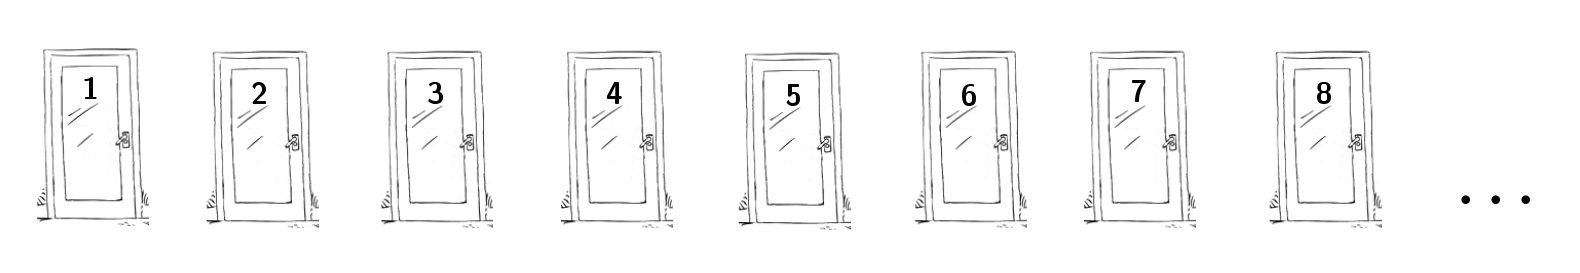
\includegraphics[scale=1.2]{door1}
\end{center}

\begin{enumerate}
\item Переселим туриста из 1 номера во 2 номер, туриста из 2 номера в 3 номер, туриста из 3 номера в 4 номер и так далее. В итоге освободится место для еще одного туриста.

\begin{center}
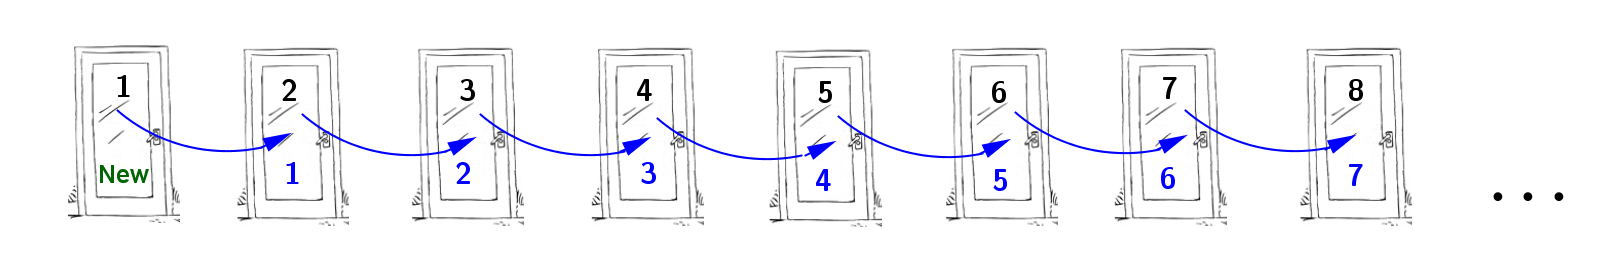
\includegraphics[scale=1.2]{door2}
\end{center}

\item Переселим туриста из 1 номера во 2 номер, из 2 номера в 4 номер, из 3 номера в 6 номер, из 4 номера в 8 номер, из 5 номера в 10 номер и так далее. В итоге освободится счётное количество номеров для дополнительного счётного количества туристов.

\begin{center}
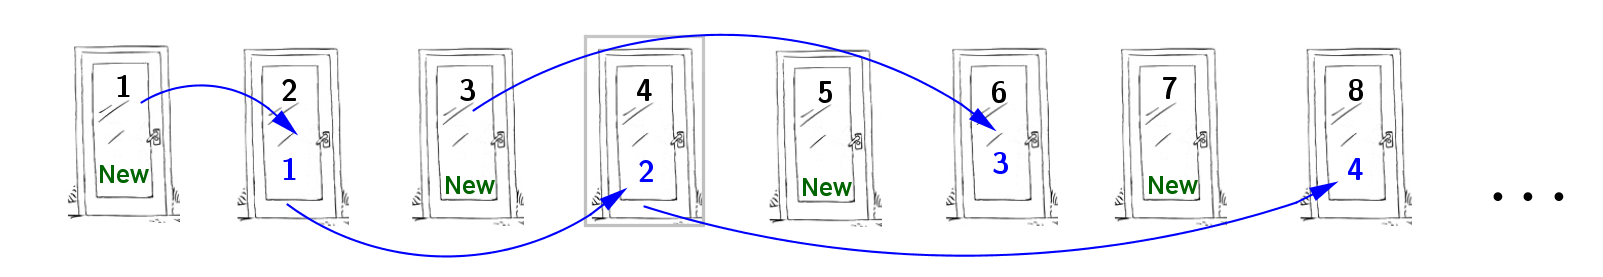
\includegraphics[scale=1.2]{door3}
\end{center}

\end{enumerate}

При решении задачи мы неявно оперировали тем фактом, что если из счётного множества удалить конечное или счётное множество, то исходное множество останется счётным. Если в счётное множество добавить конечное или счётное множество, то новое множество снова будет счётным. Чтобы доказать это достаточно построить взаимно-однозначные соответствия по аналогии с тем, как мы сделали это с жильцами.

\end{sol}
\end{problem}

\begin{problem}
Пусть $A$ --- список всех подмножеств натуральных чисел, а $S$ --- множество бесконечных последовательностей из 0 и 1. Для примера: $\{5,6,178\} \in A, \mbox{ } 0101010101010101 \ldots \in S$. Сравните мощности множеств $A$ и $S$, мощности множеств $\NN$ и $S$.
\begin{sol}
Сопоставим каждой последовательности из нулей и единиц элемент списка $A$. Если в данный элемент списка входит  натуральное число $n$, то будем ставить в последовательности на месте $n$ единицу.

 \begin{center}
\definecolor{qqqqff}{rgb}{0.,0.,1.}
\definecolor{qqttcc}{rgb}{0.,0.2,0.8}
\definecolor{qqqqcc}{rgb}{0.,0.,0.8}
\begin{tikzpicture}[line cap=round,line join=round,>=triangle 45,x=1cm,y=1cm]
\clip(-0.7941728581796409,-2.9900066347568117) rectangle (10.560863242043467,3.5563131098557585);
\draw [rotate around={90.:(2.,0.)},line width=1.6pt,color=qqqqcc] (2.,0.) ellipse (2.7489679841754673cm and 1.8859546595880108cm);
\draw [rotate around={90.:(8,0.)},line width=1.6pt,color=qqttcc] (8,0.) ellipse (2.7489679841754686cm and 1.885954659588012cm);
\draw [->] (2.,1.5) -- (7.5,1.5);
\draw [->,line width=0.4pt] (7.5,1.5) -- (2.,1.5);
\draw [->,line width=0.4pt] (2.,0.5) -- (7.5,0.5);
\draw [->,line width=0.4pt] (7.5,0.5) -- (2.,0.5);
\draw [->,line width=0.4pt] (2.,-0.5) -- (7.5,-0.5);
\draw [->,line width=0.4pt] (7.5,-0.5) -- (2.,-0.5);
\draw [->,line width=0.4pt] (2.,-1.5) -- (7.5,-1.5);
\draw [->,line width=0.4pt] (7.5,-1.5) -- (2.,-1.5);
\draw (1.1,1.9803472454119917) node[anchor=north west] {$\mathbf{\varnothing}$};
\draw (0.9,0.9835825106355921) node[anchor=north west] {$\mathbf{\{1\}}$};
\draw (0.7,-0.04012181156719667) node[anchor=north west] {$\mathbf{\{1,3\}}$};
\draw (0.7,-1.009946958917207) node[anchor=north west] {$\mathbf{\{2,4\}}$};
\draw (7.5,1.966877451698797) node[anchor=north west] {\small{$\mathbf{00000\ldots}$}};
\draw (7.5,0.9701127169223975) node[anchor=north west] {\small{$\mathbf{10000\ldots}$}};
\draw (7.5,-0.02665201785400208) node[anchor=north west] {\small{$\mathbf{10100\ldots}$}};
\draw (7.5,-1.0503563400567908) node[anchor=north west] {\small{$\mathbf{01010\ldots}$}};
\draw (7.7,-1.8) node[anchor=north west] {$\dots$};
\draw (1.7,-1.8) node[anchor=north west] {$\dots$};
\begin{scriptsize}
\draw [fill=qqqqff] (2.,1.5) circle (2.0pt);
\draw [fill=qqqqff] (2.,0.5) circle (2.0pt);
\draw [fill=qqqqff] (2.,-0.5) circle (2.0pt);
\draw [fill=qqqqff] (2.,-1.5) circle (2.0pt);
\draw [fill=qqqqff] (7.5,1.5) circle (2.0pt);
\draw [fill=qqqqff] (7.5,0.5) circle (2.0pt);
\draw [fill=qqqqff] (7.5,-0.5) circle (2.0pt);
\draw [fill=qqqqff] (7.5,-1.5) circle (2.0pt);
\end{scriptsize}
\end{tikzpicture}
\end{center}

Таким образом каждой последовательности будет соответствовать единственный элемент списка. Множества $A$ b $S$ равномощны.

Так как мощность списка из подмножеств множества больше мощности множества и $|A|=|S|$, то $|\NN|<|S|$.
\end{sol}
\end{problem}


\begin{problem}
Чудо-чудное, диво-дивное! Существует ли список $S$ всех возможных мощностей?
\begin{sol}
Нет! От противного, допустим $S$ существует. Для каждого $s\in S$ существует множество $A_{s}$ соответствующей мощности. Построим множество $A=\cup_{s}A_{s}$. Здесь используется аксиома выбора. И теперь построим множество $B=2^{A}$. Оно больше любого из $A_{s}$! Значит оно не было упомянуто в списке $S$.
\end{sol}
\end{problem}

\begin{problem}
Декартово произведение счётного количества счётных множеств
является счётным множеством. Да или нет?
\begin{sol}
Нет. Пусть $S$ --- множество всех последовательностей из нулей и единиц. $A = \NN \times \NN \times \NN \times \ldots$ --- декартово произведение счетного количества счетных множеств.

Тогда мощность множества $S$ точно не больше мощности множества $A$, так как в множестве $A$ существует подмножество последовательностей, состоящих только из нулей и единиц, для которого можно построить взаимно-однозначное соответствие с $S$.

Значит множеству $S$ поставлено во взаимно-однозначное соответствие подмножество $A$ и $|A| \ge |S|$.

В свою очередь мощность множества $A$ точно не больше мощности множества $S$. Построим следующее взаимно-однозначное соответствие.

\begin{center}
\definecolor{qqqqff}{rgb}{0.,0.,1.}
\definecolor{qqttcc}{rgb}{0.,0.2,0.8}
\definecolor{qqqqcc}{rgb}{0.,0.,0.8}
\begin{tikzpicture}[line cap=round,line join=round,>=triangle 45,x=1cm,y=1cm]
\clip(-0.7941728581796409,-2.9900066347568117) rectangle (10.560863242043467,3.5563131098557585);
\draw [rotate around={90.:(2.,0.)},line width=1.6pt,color=qqqqcc] (2.,0.) ellipse (2.7489679841754673cm and 1.8859546595880108cm);
\draw [rotate around={90.:(8,0.)},line width=1.6pt,color=qqttcc] (8,0.) ellipse (2.7489679841754686cm and 1.885954659588012cm);
\draw [->] (2.,1.5) -- (7.5,1.5);
\draw [->,line width=0.4pt] (7.5,1.5) -- (2.,1.5);
\draw [->,line width=0.4pt] (2.,0.5) -- (7.5,0.5);
\draw [->,line width=0.4pt] (7.5,0.5) -- (2.,0.5);
\draw [->,line width=0.4pt] (2.,-0.5) -- (7.5,-0.5);
\draw [->,line width=0.4pt] (7.5,-0.5) -- (2.,-0.5);
\draw [->,line width=0.4pt] (2.,-1.5) -- (7.5,-1.5);
\draw [->,line width=0.4pt] (7.5,-1.5) -- (2.,-1.5);
\draw (1.5,1.9803472454119917) node[anchor=north west] {$\mathbf{1}$};
\draw (1.5,0.9835825106355921) node[anchor=north west] {$\mathbf{2}$};
\draw (1.5,-0.04012181156719667) node[anchor=north west] {$\mathbf{3}$};
\draw (1.5,-1.009946958917207) node[anchor=north west] {$\mathbf{4}$};
\draw (7.5,1.966877451698797) node[anchor=north west] {\small{$\mathbf{10}$}};
\draw (7.5,0.9701127169223975) node[anchor=north west] {\small{$\mathbf{110}$}};
\draw (7.5,-0.02665201785400208) node[anchor=north west] {\small{$\mathbf{1110}$}};
\draw (7.5,-1.0503563400567908) node[anchor=north west] {\small{$\mathbf{11110}$}};
\draw (7.7,-1.8) node[anchor=north west] {$\dots$};
\draw (1.7,-1.8) node[anchor=north west] {$\dots$};
\begin{scriptsize}
\draw [fill=qqqqff] (2.,1.5) circle (2.0pt);
\draw [fill=qqqqff] (2.,0.5) circle (2.0pt);
\draw [fill=qqqqff] (2.,-0.5) circle (2.0pt);
\draw [fill=qqqqff] (2.,-1.5) circle (2.0pt);
\draw [fill=qqqqff] (7.5,1.5) circle (2.0pt);
\draw [fill=qqqqff] (7.5,0.5) circle (2.0pt);
\draw [fill=qqqqff] (7.5,-0.5) circle (2.0pt);
\draw [fill=qqqqff] (7.5,-1.5) circle (2.0pt);
\end{scriptsize}
\end{tikzpicture}
\end{center}

Тогда, например, элементу $(1,2,2,3,\ldots) \in A$ будет соответствовать элемент $101101101110\ldots$. Каким бы ни был элемент из множества $A$, в последовательности никогда не будет двух нулей подряд. Значит множеству $A$ поставлено во взаимно-однозначное соответствие какое-то подмножество $S$ и $|A| \le |S|$.

Так как $|A| \ge |S|$ и $|A| \le |S|$, мощности множеств совпадают, $|A|=|S|$. Оба множества имеют мощность континуум.

При решении этой задачи можно просто привести следующий контр-пример. Бесконечные вправо последовательности из 0 и 1 --- это декартово произведение счётного количества $A_{i}$, где каждое $A_{i}=\{0,1\}$
\end{sol}
\end{problem}

\begin{problem}\label{upr1}
Постройте взаимно-однозначное соответствие между множествами $(0;1) \times (0;1)$ и $\RR^{2}$. С помощью построенного соответствия докажите, что множества $[0;1] \times [0;1]$ и $\RR^{2}$ равномощны.
\begin{sol}
Для того, чтобы каждому элементу из множества $(0;1) \times (0;1)$ поставить единственным образом в соответствие элемент из $\RR^{2}$ нужно найти такое отображение, что:
\[ \lim_{x \to 0} f(x) = - \infty \text{ и } \lim_{x \to 1} f(x) = + \infty.\] Аналогичное отображение нужно подобрать для переменной $y$. Первое, что приходит в голову --- начать экспериментировать с экспонентами и тангенсами, но это плохая идея.

Попробуем не заморачиваться. Чтобы $\lim_{x \to 0} f(x) = - \infty$ достаточно взять функцию $-\dfrac{1}{x^2}$. Чтобы получить  $\lim_{x \to 1} f(x) = + \infty$ достаточно взять функцию $\dfrac{1}{(x-1)^2}$. Тогда для функции $-\dfrac{1}{x^2} + \dfrac{1}{(x-1)^2}$ получаем:

\[\lim_{x \to 0} \left(-\frac{1}{x^2} + \dfrac{1}{(x-1)^2}\right) = -\infty -1 = -\infty,\]

\[\lim_{x \to 1} \left(-\frac{1}{x^2} + \dfrac{1}{(x-1)^2}\right) = -1 + \infty = +\infty,\].

Таким образом по правилу $(x,y) \leftrightarrow \left(-\dfrac{1}{x^2} + \dfrac{1}{(x-1)^2},-\dfrac{1}{y^2} + \dfrac{1}{(y-1)^2}\right)$ мы каждому элементу из $(0;1) \times (0;1)$ поставим в соответствие элемент из $\RR^{2}$.

Для того, чтобы доказать, что множества $[0;1] \times [0;1]$ и $\RR^{2}$ равномощны, нам нужно построить взаимно-однозначное соответствие между этими двумя множествами.

\begin{center}
\definecolor{qqqqff}{rgb}{0.,0.,1.}
\definecolor{qqwuqq}{rgb}{0.,0.39215686274509803,0.}
\definecolor{ffqqqq}{rgb}{1.,0.,0.}
\begin{tikzpicture}[line cap=round,line join=round,>=triangle 45,x=0.8cm,y=0.8cm]
\clip(-4.111289704910403,-1.5128932941321722) rectangle (10.605912648926926,6.79873266366131);
\fill[line width=1.6pt,color=qqwuqq,fill=qqwuqq,fill opacity=0.1] (0.,4.) -- (0.,1.) -- (-3.,1.) -- (-3.,4.) -- cycle;
\fill[color=qqqqff,fill=qqqqff,fill opacity=0.1] (5.94,5.76) -- (4.66,5.58) -- (3.4,5.16) -- (3.06,4.02) -- (3.06,2.74) -- (2.94,1.7) -- (3.,0.82) -- (3.46,-0.18) -- (4.18,-0.74) -- (5.4,-0.84) -- (6.96,-0.9) -- (7.98,-0.42) -- (8.7,0.5) -- (9.18,1.76) -- (9.4,3.16) -- (9.18,4.4) -- (8.58,5.26) -- (7.58,5.7) -- (6.5,5.72) -- cycle;
\draw [line width=1.6pt,color=qqwuqq] (0.,4.)-- (0.,1.);
\draw [line width=1.6pt,color=qqwuqq] (0.,1.)-- (-3.,1.);
\draw [line width=1.6pt,color=qqwuqq] (-3.,1.)-- (-3.,4.);
\draw [line width=1.6pt,color=qqwuqq] (-3.,4.)-- (0.,4.);
\draw [line width=1.6pt,dash pattern=on 8pt off 8pt,color=qqqqff] (6.059421412128413,5.75334642883689)-- (6.06,-0.84);
\draw (-3.1,3.0178802542890866) node[anchor=north west] {$\mathbf{[0;1] \times [0;1]}$};
\draw (3.9816092539937755,2.142972258731878) node[anchor=north west] {$\mathbf{\RR^2}$};
\draw [->,line width=0.4pt,color=qqwuqq] (-3.,4.) -- (0.015114492880381025,3.969771014239238);
\draw [->,line width=0.4pt,color=qqwuqq] (0.015114492880381183,0.9697710142392378) -- (0.015114492880381185,3.969771014239238);
\begin{scriptsize}
\draw [fill=ffqqqq] (0.,4.) circle (2.5pt);
\end{scriptsize}
\end{tikzpicture}
\end{center}

В предыдущем пункте задачи мы нашли отображение, которое переводит все точки квадрата в точки плоскости, но при этом мы не нашли ни одной точки, которой в соответствие можно было бы поставить границу квадрата. Возьмем на плоскости произвольную прямую. Прямая равномощна полупрямой с выколотым началом. То есть между ними можно установить взаимно-однозначное соответствие.

\begin{center}
\definecolor{wwqqzz}{rgb}{0.4,0.,0.6}
\definecolor{qqqqff}{rgb}{0.,0.,1.}
\definecolor{qqwuqq}{rgb}{0.,0.39215686274509803,0.}
\definecolor{ffqqqq}{rgb}{1.,0.,0.}
\begin{tikzpicture}[line cap=round,line join=round,>=triangle 45,x=0.8cm,y=0.8cm]
\clip(-3.525776137780285,-1.4871732097146722) rectangle (11.158053875118634,6.026209026184774);
\fill[line width=1.6pt,color=qqwuqq,fill=qqwuqq,fill opacity=0.1] (0.,4.) -- (0.,1.) -- (-3.,1.) -- (-3.,4.) -- cycle;
\fill[color=qqqqff,fill=qqqqff,fill opacity=0.1] (5.94,5.76) -- (4.66,5.58) -- (3.4,5.16) -- (3.06,4.02) -- (3.06,2.74) -- (2.94,1.7) -- (3.,0.82) -- (3.46,-0.18) -- (4.18,-0.74) -- (5.4,-0.84) -- (6.96,-0.9) -- (7.98,-0.42) -- (8.7,0.5) -- (9.18,1.76) -- (9.4,3.16) -- (9.18,4.4) -- (8.58,5.26) -- (7.58,5.7) -- (6.5,5.72) -- cycle;
\draw [line width=1.6pt,color=qqwuqq] (0.,4.)-- (0.,1.);
\draw [line width=1.6pt,color=qqwuqq] (0.,1.)-- (-3.,1.);
\draw [line width=1.6pt,color=qqwuqq] (-3.,1.)-- (-3.,4.);
\draw [line width=1.6pt,color=qqwuqq] (-3.,4.)-- (0.,4.);
\draw (-3.1,3.0178802542890866) node[anchor=north west] {$\mathbf{[0;1] \times [0;1]}$};
\draw (3.9816092539937755,2.142972258731878) node[anchor=north west] {$\mathbf{\RR^2}$};
\draw [line width=1.6pt,dotted,color=wwqqzz] (5.9813989581245375,2.04923211635075)-- (5.9813989581245375,5.673850955087756);
\draw [->,line width=1.6pt,dash pattern=on 8pt off 8pt,color=qqqqff] (6.012485672022963,-0.8729189901012959) -- (5.981398958124537,2.049232116350843);
\draw [->,line width=0.4pt,color=qqwuqq] (-3.,4.) -- (0.015114492880381025,3.969771014239238);
\draw [->,line width=0.4pt,color=qqwuqq] (0.015114492880381183,0.9697710142392378) -- (0.015114492880381185,3.969771014239238);
\begin{scriptsize}
\draw [fill=ffqqqq] (0.,4.) circle (2.5pt);
\end{scriptsize}
\end{tikzpicture}
\end{center}

Любой интервал равномощен полупрямой. Сопоставим между собой границу квадрата и незанятую полупрямую с включённым началом.

\begin{center}
\definecolor{qqqqff}{rgb}{0.,0.,1.}
\definecolor{qqwuqq}{rgb}{0.,0.39215686274509803,0.}
\definecolor{ffqqqq}{rgb}{1.,0.,0.}
\begin{tikzpicture}[line cap=round,line join=round,>=triangle 45,x=0.8cm,y=0.8cm]
\clip(-3.579776155240749,-1.1806060881890135) rectangle (9.949582062279424,5.964416424276412);
\fill[line width=1.6pt,color=qqwuqq,fill=qqwuqq,fill opacity=0.1] (0.015114492880381185,3.969771014239238) -- (0.015114492880381185,0.969771014239238) -- (-3.,1.) -- (-3.,4.) -- cycle;
\fill[color=qqqqff,fill=qqqqff,fill opacity=0.1] (5.94,5.76) -- (4.66,5.58) -- (3.4,5.16) -- (3.06,4.02) -- (3.06,2.74) -- (2.94,1.7) -- (3.,0.82) -- (3.46,-0.18) -- (4.18,-0.74) -- (5.4,-0.84) -- (6.96,-0.9) -- (7.98,-0.42) -- (8.7,0.5) -- (9.18,1.76) -- (9.4,3.16) -- (9.18,4.4) -- (8.58,5.26) -- (7.58,5.7) -- (6.5,5.72) -- cycle;
\draw [line width=1.6pt,color=qqwuqq] (0.015114492880381185,3.969771014239238)-- (0.015114492880381185,0.969771014239238);
\draw [line width=1.6pt,color=qqwuqq] (0.015114492880381185,0.969771014239238)-- (-3.,1.);
\draw [line width=1.6pt,color=qqwuqq] (-3.,1.)-- (-3.,4.);
\draw [line width=1.6pt,color=qqwuqq] (-3.,4.)-- (0.015114492880381185,3.969771014239238);
\draw (-3.1,3.0178802542890866) node[anchor=north west] {$\mathbf{[0;1] \times [0;1]}$};
\draw (3.9816092539937755,2.142972258731878) node[anchor=north west] {$\mathbf{\RR^2}$};
\draw [->,line width=1.6pt,dash pattern=on 7pt off 7pt,color=qqqqff] (6.012485672022963,-0.8729189901012959) -- (5.981398958124537,2.049232116350843);
\draw [->,line width=0.4pt,color=qqwuqq] (-3.,4.) -- (0.015114492880381025,3.969771014239238);
\draw [->,line width=0.4pt,color=qqwuqq] (0.015114492880381183,0.9697710142392378) -- (0.015114492880381185,3.969771014239238);
\draw [->,line width=1.6pt,color=qqwuqq] (5.98314370935182,5.7470773364447645) -- (6.,2.);
\begin{scriptsize}
\draw [fill=ffqqqq] (0.015114492880381185,3.969771014239238) circle (2.5pt);
\draw [fill=ffqqqq] (6.,2.) circle (2.5pt);
\end{scriptsize}
\end{tikzpicture}
\end{center}

Проделав всё это мы сопоставили плоскости квадрат с его границей. Заметим, что, используя это отображение, можно доказать равномощность $[0;1]$ и $\RR$.

\end{sol}
\end{problem}



\subsection{Топология вещественной прямой.}

Всякий рыцарь, желающий завоевать сердце принцессы знанием  стохастического анализа, должен проникнуться древним искусством, пришедшим к нам из 1847 года, а именно топологией!

На всём пути изучения материала этой книги рыцарь будет чаще всего сталкиваться с множеством действительных чисел. Понимание того, как могут быть устроены множества на вещественной прямой является основополагающим для большинства последующих тем учебника. Поэтому авторы не видят смысла продолжать повествования, не познакомив рыцаря с замечательной во всех смыслах темой - Топологией вещественной прямой!

\begin{mydef} \indef{Окрестностью}  \index{окрестность} $U(a)$ точки $a$ называется любой интервал, содержащий точку $a$. Чаще всего рассматривают симметричную окрестность радиуса $\dt$, $U_{\dt} (a)$ или $(a-\dt,a+\dt)$.
\end{mydef}

\begin{rem}
Отметим, что любую произвольную окрестность можно превратить в симметричную $\dt$-окрестность.
\end{rem}

\begin{mydef}
 \indef{Проколотой окрестностью}  \index{проколотая окрестность} точки $a$ называется окрестность точки $a$, из~которой исключена сама точка $a$, т.е. $\dot U(a) = U(a) \setminus a.$
\end{mydef}

\begin{mydef} Точка $a$ называется \indef{внутренней точкой множества $A$}, \index{внутренняя точка} если существует такая окрестность точки $a$, что эта окрестность целиком лежит в~$A$.
\end{mydef}

\begin{mydef} Точка $a$ называется \indef{граничной точкой множества $A$},  \index{граничная точка} если для~любой окрестности точки $a$ верно, что её пересечение с множеством $A$ не пусто и её пересечение с дополнением множества $A$ также не пусто, т.е.
$U(a) \cap A \ne \varnothing $ и $U(a) \cap (\R \setminus A)\ne \varnothing$.
\end{mydef}

\begin{mydef} Точка $a$ называется \indef{изолированной точкой множества $A$},  \index{изолированная точка} если существует такая окрестность точки $a$, что её пересечение с множеством $A$ равно точке $a$, т.е. $U(a) \cap A = a$.
\end{mydef}



\begin{figure}[H]\label{dots}
\begin{center}
\definecolor{qqqqff}{rgb}{0.,0.,1.}
\begin{tikzpicture}[line cap=round,line join=round,>=triangle 45,x=1.0cm,y=1.0cm]
\clip(-1.16,1.06) rectangle (10.26,4.98);
\draw (-1.,3.)-- (10.,3.);
\draw [->,line width=1.2pt,,color=qqqqff] (1.,3.) -- (4.26,3.);
\draw [->,line width=1.2pt,color=qqqqff] (4.26,3.) -- (0.68,3.);
\draw (0.58,3.84) node[anchor=north west] {$\mathbf{2}$};
\draw (3.9,3.88) node[anchor=north west] {$\mathbf{4}$};
\draw (5.84,3.9) node[anchor=north west] {$\mathbf{7}$};
\draw (1.16,4.32) node[anchor=north west] {$\text{внутренние точки}$};
\draw (1.4,1.8) node[anchor=north west] {$\text{граничные точки}$};
\draw (5.98,1.82) node[anchor=north west] {$\text{изолированная точка}$};
\draw [->] (2.28,3.86) -- (2.32,3.14);
\draw [->] (2.08,2.02) -- (0.86,2.84);
\draw [->] (2.96,2.02) -- (4.08,2.84);
\draw [->] (7.62,2.14) -- (6.46,2.8);
\draw [->] (3.914,1.988) -- (5.96,2.802);
\begin{scriptsize}
\draw [fill=qqqqff] (6.26,3.) circle (2.5pt);
\end{scriptsize}
\end{tikzpicture}
\end{center}
\caption{Внутренние, граничные и изолированные точки}
\end{figure}


\begin{myex}\label{pr124}
Если $A = (2,4) \cup \{7\}$, то~точка $a=0$ является изолированной, точки $\{2,4,7\}$ являются граничными, точки $(2,4)$ являются внутренними. Всё~это иллюстрирует рисунок \ref{dots}.
\end{myex}

\begin{mydef} Точка $a$ называется \indef{предельной точкой множества $A$},  \index{предельная точка} если  пересечение любой её проколотой окрестности с множеством $A$ не пусто, т.е. $\forall \dot U(a) \mbox{ } \dot U(a) \cap A \ne \varnothing$.
\end{mydef}

\begin{myex}
\mbox{ }

\begin{enumerate}
\item У~множества в~примере \ref{pr124} все точки, кроме изолированной будут предельными.
\item У~множества натуральных чисел нет предельных точек.
\end{enumerate}
\end{myex}

\begin{myth} Если $a$ --- предельная точка множества $A$, то~пересечение любой проколотой окрестности с~этим множеством $A$ --- бесконечное множество.
\end{myth}
\begin{proof}
Рассмотрим произвольную $\dt$-окрестность точки $a$. В~проколотой $\dt$-окрестности точки $a$ выберем произвольную точку $a_1$. Теперь положим  $\dt_1=|a_1-a|$. В проколотой $\dt_1$-окрестности выберем точку $a_2$. Точка $a_2$ будет отлична от точки $a_1$. Теперь положим  $\dt_2=|a_2-a|$. И так далее $\ldots$ Полученный набор точек $a_i$ завершает доказательство.
\end{proof}

\begin{cor}Конечное множество не~имеет предельных точек.
\end{cor}

\begin{mydef} Множество называется \indef{открытым},  \index{открытое множество} если все его точки – внутренние. Множество называется \indef{замкнутым},  \index{замкнутое множество} если оно является дополнением к~открытому.
\end{mydef}

\begin{myex}
Множество $(2,4)$ открытое, множество $[2,4]$ замкнутое, множество $(2,4) \cup \{7\}$ не~открытое, не~замкнутое. Множества $\R$ и $\varnothing$ одновременно и замкнутые и открытые.
\end{myex}

\begin{myex}
На плоскости, $\RR^2$, можно привести следующие примеры замкнутых и открытых множеств.

\begin{center}
\definecolor{qqqqff}{rgb}{0.,0.,1.}
\begin{tikzpicture}[line cap=round,line join=round,>=triangle 45,x=0.7cm,y=0.7cm]
\clip(-2.62284432315135,0.49266110424500137) rectangle (20.528106668904982,6.173567645183906);
\fill[line width=1.6pt,color=qqqqff,fill=qqqqff,fill opacity=0.1] (-0.762885049066963,5.018402561372592) -- (-1.3097423317102617,4.755911065703809) -- (-1.7253538665191686,4.362173822200633) -- (-1.9440967795764879,3.8590651221687984) -- (-2.0097196534936836,3.159087800385376) -- (-1.7691024491306324,2.5466076438248817) -- (-1.4191137882389213,2.1747446916274384) -- (-0.8285079229841589,1.7591331568185316) -- (-0.2160277664236644,1.5841388263726761) -- (0.4839495553597578,1.3435216220096247) -- (1.18392687714318,1.234150165480965) -- (1.8401556163151382,1.168527291563769) -- (2.387012898958437,1.146653000258037) -- (2.824498725073076,1.212275874175233) -- (3.524476046856498,1.4966416611497484) -- (4.005710455582601,1.977876069875851) -- (4.33382482516858,2.393487604684758) -- (4.421321990391507,2.962219178633789) -- (4.443196281697239,3.3778307134426955) -- (4.3775734077800434,3.662196500417211) -- (4.136956203416992,4.405922404812098) -- (3.743218959913817,4.8652825222324685) -- (3.3713560077163742,5.10589972659552) -- (2.86824730768454,5.455888387487231) -- (2.408887190264169,5.4996369700986945) -- (2.08077282067819,5.455888387487231) -- (0.6589438858056134,5.215271183124179) -- (-0.369147805563788,5.062151143984056) -- cycle;
\fill[line width=1.6pt,dash pattern=on 6pt off 6pt,color=qqqqff,fill=qqqqff,fill opacity=0.1] (7.286854151442392,4.930905396149663) -- (6.739996868799094,4.66841390048088) -- (6.324385333990187,4.2746766569777055) -- (6.105642420932868,3.7715679569458698) -- (6.040019547015672,3.071590635162448) -- (6.280636751378723,2.4591104786019535) -- (6.630625412270434,2.0872475264045103) -- (7.221231277525196,1.6716359915956036) -- (7.833711434085689,1.4966416611497482) -- (8.533688755869111,1.2560244567866965) -- (9.233666077652533,1.1466530002580368) -- (9.889894816824494,1.0810301263408406) -- (10.436752099467792,1.0591558350351087) -- (10.874237925582431,1.124778708952305) -- (11.574215247365853,1.4091444959268205) -- (12.055449656091959,1.890378904652923) -- (12.383564025677938,2.30599043946183) -- (12.471061190900866,2.8747220134108606) -- (12.492935482206601,3.2903335482197673) -- (12.427312608289402,3.5746993351942824) -- (12.186695403926354,4.318425239589169) -- (11.792958160423172,4.77778535700954) -- (11.42109520822573,5.018402561372591) -- (10.917986508193895,5.368391222264302) -- (10.458626390773524,5.412139804875766) -- (10.130512021187545,5.368391222264302) -- (8.708683086314966,5.127774017901251) -- (7.680591394945567,4.974653978761127) -- cycle;
\fill[line width=1.6pt,color=qqqqff,fill=qqqqff,fill opacity=0.1] (14.833484651919914,4.712162483092345) -- (14.286627369276616,4.449670987423562) -- (13.871015834467709,4.055933743920386) -- (13.65227292141039,3.5528250438885514) -- (13.586650047493194,2.852847722105129) -- (13.827267251856245,2.240367565544635) -- (14.177255912747956,1.8685046133471916) -- (14.767861778002718,1.4528930785382848) -- (15.380341934563212,1.2778987480924293) -- (16.080319256346634,1.0372815437293779) -- (16.780296578130056,0.9279100872007182) -- (17.436525317302014,0.862287213283522) -- (17.983382599945315,0.84041292197779) -- (18.420868426059954,0.9060357958949863) -- (19.120845747843376,1.1904015828695016) -- (19.602080156569478,1.6716359915956043) -- (19.930194526155457,2.0872475264045116) -- (20.017691691378385,2.655979100353542) -- (20.039565982684117,3.071590635162449) -- (19.97394310876692,3.355956422136964) -- (19.73332590440387,4.099682326531851) -- (19.339588660900695,4.5590424439522215) -- (18.967725708703252,4.799659648315273) -- (18.464617008671418,5.149648309206984) -- (18.005256891251044,5.193396891818447) -- (17.67714252166507,5.149648309206984) -- (16.25531358679249,4.909031104843932) -- (15.227221895423089,4.755911065703809) -- cycle;
\draw [line width=1.6pt,color=qqqqff] (-0.762885049066963,5.018402561372592)-- (-1.3097423317102617,4.755911065703809);
\draw [line width=1.6pt,color=qqqqff] (-1.3097423317102617,4.755911065703809)-- (-1.7253538665191686,4.362173822200633);
\draw [line width=1.6pt,color=qqqqff] (-1.7253538665191686,4.362173822200633)-- (-1.9440967795764879,3.8590651221687984);
\draw [line width=1.6pt,color=qqqqff] (-1.9440967795764879,3.8590651221687984)-- (-2.0097196534936836,3.159087800385376);
\draw [line width=1.6pt,color=qqqqff] (-2.0097196534936836,3.159087800385376)-- (-1.7691024491306324,2.5466076438248817);
\draw [line width=1.6pt,color=qqqqff] (-1.7691024491306324,2.5466076438248817)-- (-1.4191137882389213,2.1747446916274384);
\draw [line width=1.6pt,color=qqqqff] (-1.4191137882389213,2.1747446916274384)-- (-0.8285079229841589,1.7591331568185316);
\draw [line width=1.6pt,color=qqqqff] (-0.8285079229841589,1.7591331568185316)-- (-0.2160277664236644,1.5841388263726761);
\draw [line width=1.6pt,color=qqqqff] (-0.2160277664236644,1.5841388263726761)-- (0.4839495553597578,1.3435216220096247);
\draw [line width=1.6pt,color=qqqqff] (0.4839495553597578,1.3435216220096247)-- (1.18392687714318,1.234150165480965);
\draw [line width=1.6pt,color=qqqqff] (1.18392687714318,1.234150165480965)-- (1.8401556163151382,1.168527291563769);
\draw [line width=1.6pt,color=qqqqff] (1.8401556163151382,1.168527291563769)-- (2.387012898958437,1.146653000258037);
\draw [line width=1.6pt,color=qqqqff] (2.387012898958437,1.146653000258037)-- (2.824498725073076,1.212275874175233);
\draw [line width=1.6pt,color=qqqqff] (2.824498725073076,1.212275874175233)-- (3.524476046856498,1.4966416611497484);
\draw [line width=1.6pt,color=qqqqff] (3.524476046856498,1.4966416611497484)-- (4.005710455582601,1.977876069875851);
\draw [line width=1.6pt,color=qqqqff] (4.005710455582601,1.977876069875851)-- (4.33382482516858,2.393487604684758);
\draw [line width=1.6pt,color=qqqqff] (4.33382482516858,2.393487604684758)-- (4.421321990391507,2.962219178633789);
\draw [line width=1.6pt,color=qqqqff] (4.421321990391507,2.962219178633789)-- (4.443196281697239,3.3778307134426955);
\draw [line width=1.6pt,color=qqqqff] (4.443196281697239,3.3778307134426955)-- (4.3775734077800434,3.662196500417211);
\draw [line width=1.6pt,color=qqqqff] (4.3775734077800434,3.662196500417211)-- (4.136956203416992,4.405922404812098);
\draw [line width=1.6pt,color=qqqqff] (4.136956203416992,4.405922404812098)-- (3.743218959913817,4.8652825222324685);
\draw [line width=1.6pt,color=qqqqff] (3.743218959913817,4.8652825222324685)-- (3.3713560077163742,5.10589972659552);
\draw [line width=1.6pt,color=qqqqff] (3.3713560077163742,5.10589972659552)-- (2.86824730768454,5.455888387487231);
\draw [line width=1.6pt,color=qqqqff] (2.86824730768454,5.455888387487231)-- (2.408887190264169,5.4996369700986945);
\draw [line width=1.6pt,color=qqqqff] (2.408887190264169,5.4996369700986945)-- (2.08077282067819,5.455888387487231);
\draw [line width=1.6pt,color=qqqqff] (2.08077282067819,5.455888387487231)-- (0.6589438858056134,5.215271183124179);
\draw [line width=1.6pt,color=qqqqff] (0.6589438858056134,5.215271183124179)-- (-0.369147805563788,5.062151143984056);
\draw [line width=1.6pt,color=qqqqff] (-0.369147805563788,5.062151143984056)-- (-0.762885049066963,5.018402561372592);
\draw [line width=1.6pt,color=qqqqff] (14.833484651919914,4.712162483092345)-- (14.286627369276616,4.449670987423562);
\draw [line width=1.6pt,color=qqqqff] (14.286627369276616,4.449670987423562)-- (13.871015834467709,4.055933743920386);
\draw [line width=1.6pt,color=qqqqff] (13.871015834467709,4.055933743920386)-- (13.65227292141039,3.5528250438885514);
\draw [line width=1.6pt,color=qqqqff] (13.65227292141039,3.5528250438885514)-- (13.586650047493194,2.852847722105129);
\draw [line width=1.6pt,color=qqqqff] (13.586650047493194,2.852847722105129)-- (13.827267251856245,2.240367565544635);
\draw [line width=1.6pt,color=qqqqff] (13.827267251856245,2.240367565544635)-- (14.177255912747956,1.8685046133471916);
\draw [line width=1.6pt,color=qqqqff] (14.177255912747956,1.8685046133471916)-- (14.767861778002718,1.4528930785382848);
\draw [line width=1.6pt,color=qqqqff] (14.767861778002718,1.4528930785382848)-- (15.380341934563212,1.2778987480924293);
\draw [line width=1.6pt,color=qqqqff] (15.380341934563212,1.2778987480924293)-- (16.080319256346634,1.0372815437293779);
\draw [line width=1.6pt,color=qqqqff] (16.080319256346634,1.0372815437293779)-- (16.780296578130056,0.9279100872007182);
\draw [line width=1.6pt,color=qqqqff] (18.005256891251044,5.193396891818447)-- (17.67714252166507,5.149648309206984);
\draw [line width=1.6pt,color=qqqqff] (17.67714252166507,5.149648309206984)-- (16.25531358679249,4.909031104843932);
\draw [line width=1.6pt,color=qqqqff] (16.25531358679249,4.909031104843932)-- (15.227221895423089,4.755911065703809);
\draw [line width=1.6pt,color=qqqqff] (15.227221895423089,4.755911065703809)-- (14.833484651919914,4.712162483092345);
\draw (1,3.9) node[anchor=north west] {\Large{$A_1$}};
\draw (8.8,3.9) node[anchor=north west] {\Large{$A_2$}};
\draw (16.7,3.9) node[anchor=north west] {\Large{$A_3$}};
\end{tikzpicture}
\end{center}

Множество $A_1$ --- замкнутое, множество $A_2$ --- открытое, множество $A_3$ --- ни открытое, ни замкнутое.
\end{myex}


\begin{myth} Следующие определения эквивалентны:
\begin{enumerate}
\item Множество $A$ --- замкнутое множество;
\item Множество $A$ содержит все свои граничные точки;
\item Множество $A$ содержит все свои предельные точки.
\end{enumerate}
\end{myth}

В~определении не~сказано, что предельная точка обязана принадлежать множеству $A$. Встречаются ситуации, когда предельная точка множества $A$ принадлежит самому множеству $A$, и когда она не~принадлежит множеству $A$.

\begin{myex}
Точка 0 является предельной точкой для множества $\{\frac{1}{n}\}_{n=1}^{\infty}$, однако в само множество она не входит. В то же время она является предельной точкой множества $\{\frac{1}{n}\}_{n=1}^{\infty} \cup \{0\}$, в которое она входит.
\end{myex}

\begin{mydef}
Множество $A$ называется \indef{ограниченным},  \index{ограниченное множество} если существует отрезок $[c;d]$ такой, что $A \subseteq [c;d]$.
\end{mydef}

Как известно, дорогие сыры накрывают куполообразными стеклянными крышками для того, чтобы запах этих сыров не выветривался и не распространялся, то есть пространство распространения запаха сыров ограничено. Так вот, если мы можем накрыть множество $A$ на прямой отрезком $[c;d]$, то оно будет ограничено.

\begin{myth}
Если $A$ --- бесконечное ограниченное множество, то существует предельная точка множества $A$.
\end{myth}
\begin{proof}
Рассмотрим отрезок $[c_1,d_1]=[c,d]$. Разделим его на~2 части. Хотя бы в~одну из~половин отрезка входит бесконечное множество точек $A$. Возьмем полученный отрезок $[c_2,d_2]$ и~тоже разделим его на~2~части. Хотя~бы один из~полученных отрезков $[c_3,d_3]$ тоже содержит бесконечное множество точек из~$A$. Продолжим процесс деления отрезков. В~итоге имеем систему стягивающихся отрезков. Эта система имеет единую для всех отрезков точку $c$. Докажем, что точка $c$ --- предельная точка множества $A$. Выберем произвольную $\dt$-окрестность точки $c$, $U_{\dt}(c)$.  После этого возьмем $n$ такое, чтобы длина отрезка $[a_{n+1},b_{n+1}]$, равная $\frac{d_1-c_1}{2^n}$, оказалась меньше $\dt$, т.е.

\[\frac{d_1-c_1}{2^n} < \dt \Leftrightarrow 2^n > \frac{d_1-c_1}{\dt} \Leftrightarrow n> \log_2 \frac{d_1-c_1}{\dt}.\]



Так как $[a_{n+1},b_{n+1}] \subset U_{\dt}(c)$, и так как $[a_{n+1},b_{n+1}]$ содержит, по~построению, бесконечное множество точек из $A$, проколотая окрестность $\dot U_{\dt}(c)$, также содержит бесконечное множество точек из~$A$.

\begin{center}
\begin{tikzpicture}[line cap=round,line join=round,>=triangle 45,x=1.0cm,y=1.0cm]
\clip(-1.48,2.08) rectangle (11.58,4.28);
\draw [->] (-1.,3.) -- (10.,3.);
\draw (1,3.35) node[anchor=north west] {$\mathbf{(}$};
\draw (2,3.35) node[anchor=north west] {$\mathbf{[}$};
\draw (6,3.35) node[anchor=north west] {$\mathbf{]}$};
\draw (7,3.35) node[anchor=north west] {$\mathbf{)}$};
\draw (2,3.84) node[anchor=north west] {\small{$a_{n+1}$}};
\draw (6,3.9) node[anchor=north west] {\small{$b_{n+1}$}};
\draw (0.5,3.84) node[anchor=north west] {\small{$c-\dt$}};
\draw (7,3.9) node[anchor=north west] {\small{$c+\dt$}};
\draw (9.98,3.04) node[anchor=north west] {$x$};
\begin{scriptsize}
\draw [fill=black] (4,3.) circle (1.5pt);
\draw[color=black] (4.1,3.28) node {$C$};
\end{scriptsize}
\end{tikzpicture}
\end{center}

 Итак, доказано, что произвольная окрестность $\dot U(c)$ содержит точки из~$A$. Следовательно, $c$ – предельная точка множества $A$.
\end{proof}

\begin{mydef} Пусть $A$ --- непустое подмножество прямой. Счётная система множеств $U_i$ называется \indef{покрытием}  \index{покрытие} множества $A$, если $A$ лежит в~счётном объединении множеств $U_i$.
\end{mydef}

Если в~стене есть огромная дырка, то~мы можем совершенно по-разному закрыть её коврами. Каждый способ накрыть её коврами называется покрытием.

\begin{mydef}Множество называется \indef{компактом},  \index{компакт} если из~всякого его покрытия открытыми множествами можно выделить конечное подпокрытие.  \index{подпокрытие}
\end{mydef}

Дырка в~стене будет компактом, если из~любого ее покрытия коврами можно выделить какое-то конечное число ковров, которое закроет ее.

\begin{lemma}[Гейне-Борель-Лебег] Любой отрезок является компактом.
\end{lemma}
\begin{proof}
Предположим, что наше утверждение неверное, то есть для~нашего отрезка не~существует конечного подпокрытия $I_1$. Разделим отрезок пополам. Хотя бы одна из~половин не~имеет конечного подпокрытия, так как иначе утверждение данной леммы было бы справедливо. Обозначим этот отрезок $I_2$. Его длина равна: $|I_2|=|\frac{I_1}{2}|$. И~так далее $\ldots$ Пусть отрезок $I_n$ – отрезок не допускающий конечного подпокрытия, выбранный на~$n-1$ шаге построения. Его длина равна: $|I_n|=|\frac{I_1}{2^{n-1}}|$. Получим систему стягивающихся отрезков. Она имеет единственную точку $с$. Тогда существует интервал $(\a,\b)$, накрывающий эту точку. Положим $\e = \frac{\min(\b-c,c-\a)}{2}$. Тогда существует натуральный номер $N$, такой, что $|I_N| < \e$. Получается, что отрезок $I_N$ полностью лежит внутри нашего интервала (а~это конечное подпокрытие). Все $I_N$ не~имели конечного подпокрытия. Полученное противоречие завершает доказательство.

\begin{center}
\definecolor{xdxdff}{rgb}{0.49019607843137253,0.49019607843137253,1.}
\definecolor{qqttcc}{rgb}{0.,0.2,0.8}
\definecolor{qqqqff}{rgb}{0.,0.,1.}
\begin{tikzpicture}[line cap=round,line join=round,>=triangle 45,x=0.7cm,y=0.7cm]
\clip(-5.839041719134245,-4.306004096461564) rectangle (19.022311365990657,7.121119442126534);
\draw [line width=1.6pt,color=qqttcc] (5.,4.)-- (5.,-2.);
\draw (3.,2.)-- (3.,1.5);
\draw (0.9869837476714621,2.4931363447108366)-- (1.,1.);
\draw (-1.,4.)-- (-1.,1.);
\draw [line width=0.4pt] (-3.,4.)-- (-3.,-2.);
\draw [->] (5.031950689761857,-4.019763729424955) -- (5.03206764316347,6.993922942263151);
\draw [->] (7.133807067196582,3.04369512413334) -- (7.133807067196582,5.04369512413334);
\draw [->] (7.133807067196582,5.04369512413334) -- (7.133807067196582,3.04369512413334);
\draw [->] (9.,2.642273922543591) -- (9.,-0.3577260774564066);
\draw [->] (9.,-0.3577260774564066) -- (9.,2.642273922543591);
\draw [->] (10.919715759682052,0.5887510956649606) -- (10.919715759682052,-1.4112489043350394);
\draw [->] (10.919715759682052,-1.4112489043350394) -- (10.919715759682052,0.5887510956649606);
\draw [->] (12.678863038728204,4.) -- (12.678863038728204,1.);
\draw [->] (12.678863038728204,1.) -- (12.678863038728204,4.);
\draw [->] (14.464771731213672,0.5254005660410348) -- (14.464771731213672,-3.474599433958965);
\draw [->] (14.464771731213672,-3.474599433958965) -- (14.464771731213672,0.5254005660410348);
\draw (3.5809758115051156,3.6421356950154036) node[anchor=north west] {\Large{$\mathbf{\ldots}$}};
\draw (5.427513338817945,3.615374281576087) node[anchor=north west] {\Large{$\mathbf{\ldots}$}};
\draw (-4,5.863333010478663) node[anchor=north west] {\textbf{Стягивающиеся отрезки}};
\draw (7.728994894599151,5.9436172507966125) node[anchor=north west] {\textbf{Система покрывающих интервалов}};
\draw (-3.1896617886419247,-2.1) node[anchor=north west] {$\mathbf{I_1}$};
\draw (-1.2093171941325136,0.9) node[anchor=north west] {$\mathbf{I_2}$};
\draw (0.8780730541341628,0.9) node[anchor=north west] {$\mathbf{I_3}$};
\draw (2.804894821764941,1.5) node[anchor=north west] {$\mathbf{I_4}$};
\draw [line width=0.4pt,dash pattern=on 7pt off 7pt] (5.,2.1209121214697735)-- (9.,2.132448996324028);
\draw (8.799451432171807,-0.4) node[anchor=north west] {$\mathbf{\alpha}$};
\draw (8.745928605293173,3.5618514546974542) node[anchor=north west] {$\mathbf{\beta}$};
\begin{scriptsize}
\draw [fill=qqqqff] (5.,4.) circle (2.0pt);
\draw [fill=qqqqff] (5.,-2.) circle (2.0pt);
\draw [fill=qqqqff] (3.,2.) circle (1.0pt);
\draw [fill=qqqqff] (3.,1.5) circle (1.0pt);
\draw [fill=qqqqff] (0.9869837476714621,2.4931363447108366) circle (1.0pt);
\draw [fill=qqqqff] (1.,1.) circle (1.0pt);
\draw [fill=qqqqff] (-1.,4.) circle (1.0pt);
\draw [fill=qqqqff] (-1.,1.) circle (1.0pt);
\draw [fill=qqqqff] (-3.,4.) circle (1.0pt);
\draw [fill=qqqqff] (-3.,-2.) circle (1.0pt);
\draw [fill=xdxdff] (5.,2.1209121214697735) circle (2.0pt);
\end{scriptsize}
\end{tikzpicture}
\end{center}

\end{proof}


\begin{myth}[Критерий компактности] Множество $K$ является компактом тогда и только тогда, когда множество $K$ ограничено и замкнуто.  \index{компакт}
\end{myth}

\subsubsection*{Задачи}

\begin{problem}
Верно ли, что каждая изолированная точка является граничной?
\begin{sol}
Да, это верно. Пусть точка $a$ --- изолированная точка некоторого множества A. Условие существования такой окрестности точки $a$, для~которой выполнено следующее равенство $U(a) \cap A = a$ эквивалентно тому, что для~любой окрестности точки $a$ верно, что $U(a) \cap A \ne \varnothing $, так как каким угодно интервалом точку $a$ не~накрой, то для~любой окрестности точки $a$ её пересечение с множеством $A$ будет как минимум давать точку $a$ то есть не~будет пустым. Так же это условие эквивалентно тому, что для~любой окрестности точки $a$ верно, что $U(a) \cap (\RR \setminus A)\ne \varnothing$. Это следует из~того что, если существует окрестность, для которой её пересечение с множеством A~даст точку $a$, то при удалении точки $a$ получим, что пересечение проколотой окрестности точки $a$ с~множеством A даёт пустое множество. То есть имеет место не пустое пересечение с частью множества $\RR \setminus A$. Дальнейшие попытки уменьшить или увеличить исходную окрестность не~приведут к~иному результату, что и завершает решение задачи.
\end{sol}
\end{problem}

\begin{problem}
Правда ли, что, если $a$ --- предельная точка множества $A$, то~пересечение любой проколотой окрестности точки $a$ с множеством $A$ --- бесконечное множество.
\begin{sol}
Выберем $\dt_1=1$. Выберем в~$\dot U_{\dt_1} (a)$ точку $a_1 \in A$. Положим $\dt_2 = \min (\frac{1}{2}, |a_1 - a|)$. Теперь в $\dot U_{\dt_2} (a)$ выберем точку $a_2 \in A$. Очевидно, что $a_1 \ne a_2$. Далее положим $\dt_3 = \min (\frac{1}{3}, |a_2 - a|)$, рассмотрим $\dot U_{dt_3} (a)$ и т.д. На~шаге с~номером $n$ получается точка $a_n \in A$, отличная от~предыдущих точек. Неограниченное продолжение этого процесса даёт искомое бесконечное множество.
\end{sol}
\end{problem}


\begin{problem}\label{resh_1}
Опишите все подмножества прямой, каждое из~которых является одновременно открытым и замкнутым множеством. Верно ли что других таких множеств нет?
\begin{sol}

\end{sol}
\end{problem}

\begin{problem}
Верно ли что прямую нельзя представить в~виде объединения двух непустых и непересекающихся открытых множеств? А замкнутых?


\begin{sol}
Предположим, что это верно. Тогда существуют два открытых непересекающихся и непустых множества $A$ и $B$, которые в~объединении дают всё множество действительных чисел. Рассмотрим множество $A$. Оно непусто и открыто. Тогда дополнением к~нему будет являться множество $B$, которое по~определению будет замкнутым. Получается, что $B$ одновременно и открыто, и замкнуто, и не пусто, и не всё множество действительных чисел (так как множество $A$ непусто). Получаем противоречие с задачей \ref{resh_1}.

Аналогичные рассуждения применяем для~случая двух замкнутых множеств.
\end{sol}
\end{problem}

\begin{problem}
Является ли множество  $\{\frac{1}{n}\}_{n=1}^{\infty} \cup \{0\}$ компактом? А~множество $\{\frac{1}{n}\}_{n=1}^{\infty}$?
\begin{sol}
Множество $\{\frac{1}{n}\}_{n=1}^{\infty} \cup \{0\}$ является компактом. Так как точка $0$ является предельной точкой для множества  $\{\frac{1}{n}\}_{n=1}^{\infty}$, то какой бы окрестностью мы точку ноль не покрыли (а мы её обязаны покрыть) за~пределами этой окрестности останется лишь конечное число точек исходного множества, которое мы можем покрыть конечным числом интервалов. Получается, что из всякого покрытия открытыми множествами этого множества можно выделить конечное подпокрытие. Это и соответствует определению компакта.

Множество точек  $\{\frac{1}{n}\}_{n=1}^{\infty}$ не является компактом. Достаточно предъявить покрытие $\cup_{n=1}^{\infty} \left(\frac{1}{n} - \frac{1}{10^n}; \frac{1}{n} + \frac{1}{10^n}\right)$.
Из~данного покрытия нельзя выделить конечное подпокрытие (попробовать выделить самостоятельно), а это противоречит определению компакта.
\end{sol}
\end{problem}



\subsection{Частичный предел. Верхний и нижний.}

Если есть последовательность $ (a_{n} )_{n=1}^{+ \infty},$ то, забыв порядок чисел, можно рассмотреть ее как множество точек на~числовой прямой.

\begin{rem}
Многие российские авторы записывают последовательности не в~круглых скобках $(a_{n} )_{n=1}^{+ \infty}$, а в~фигурных $\{a_{n} \}_{n=1}^{+ \infty}$. Такая запись не совсем правильная. В~фигурных скобках обычно записывают элементы, из~которых состоит множество. Каждый элемент множества уникален, и в~множестве не может быть двух одинаковых элементов. Множество $\{ 2,3,3 \}$, и множество $\{2,3\}$ одинаковы! Множество $\{\text{банан},\text{банан},\text{яблоко},\text{груша}, \text{яблоко},\text{банан}\}$, и множество $\{\text{банан},\text{яблоко},\text{груша} \}$ тоже одинаковы!

В~круглых скобках обычно записывают упорядоченную совокупность каких-то элементов. Например, координаты точки $A$ в~трехмерном пространстве, декартово произведение двух множеств, порядок в~котором мы будем поедать фрукты из~холодильника. Съесть фрукты в~порядке $(\text{банан},\text{банан},\text{яблоко},\text{груша}, \text{яблоко},\text{банан})$ и съесть фрукты в~порядке $(\text{яблоко},\text{груша},\text{яблоко},\text{банан},\text{банан},\text{банан})$ --- это совершенно разные вещи! В~такой записи очень важен порядок элементов. Более того, они могут повторяться.

Грубо говоря, посмотрев на запись в~фигурных скобках, мы понимаем что лежит в~холодильнике, посмотрев на запись в~круглых скобках, мы понимаем в~каком порядке мы эти продукты съедим!

Следуя такой логике, запись $\{1\}_{i=1}^{+\infty}$ означает ни что иное как множество, состоящее из~единственной единицы.

\[\{1\}_{i=1}^{+\infty} = \{1,1,1,1,1, \dots \} = \{1 \} \]

Запись $(1)_{i=1}^{+\infty}$ означает последовательность из~единиц.

\[(1)_{i=1}^{+\infty} = (1,1,1,1,1, \dots )\]

\end{rem}

\begin{myex} Последовательности $a_{n}=(-1)^{n}+\frac{1}{n}$ на~прямой соответствует множество точек:

\begin{center}
\begin{tikzpicture}[line cap=round,line join=round,>=triangle 45,x=0.9cm,y=0.9cm]
\clip(-1.3655521498387457,0.9854044641312166) rectangle (13.786850270031334,3.3628135394605763);
\draw [->] (-3.,2.) -- (13.,2.);
\draw (12.870258819301952,1.9163176562782551) node[anchor=north west] {$a_n$};
\draw (-0.6,1.85) node[anchor=north west] {$\mathbf{-1}$};
\draw (3.7,1.85) node[anchor=north west] {$\mathbf{0}$};
\draw (7.7,1.85) node[anchor=north west] {$\mathbf{1}$};
\draw (2.6158919642670027,2.8329091070076466) node[anchor=north west] {$\mathbf{-\frac{2}{3}}$};
\draw (0.9975351840729397,2.81858736559) node[anchor=north west] {$\mathbf{-\frac{4}{5}}$};
\draw (0.32441333744355055,2.8042656241723534) node[anchor=north west] {$\mathbf{-\frac{6}{7}}$};
\draw (-0.2914215435152523,2.81858736559) node[anchor=north west] {$\mathbf{-\frac{8}{9}}$};
\draw (11.853415178649046,2.8615525898429404) node[anchor=north west] {$\mathbf{\frac{3}{2}}$};
\draw (9.848371380178525,2.81858736559) node[anchor=north west] {$\mathbf{\frac{5}{4}}$};
\draw (8.888814705196204,2.8329091070076466) node[anchor=north west] {$\mathbf{\frac{7}{6}}$};
\draw (8.31594504849034,2.81858736559) node[anchor=north west] {$\mathbf{\frac{9}{8}}$};
\draw (7.757397133202124,2.81858736559) node[anchor=north west] {$\mathbf{\frac{11}{10}}$};
\begin{scriptsize}
\draw [color=black] (4.,2.)-- ++(-1.5pt,0 pt) -- ++(3.0pt,0 pt) ++(-1.5pt,-1.5pt) -- ++(0 pt,3.0pt);
\draw [color=black] (8.,2.)-- ++(-1.5pt,0 pt) -- ++(3.0pt,0 pt) ++(-1.5pt,-1.5pt) -- ++(0 pt,3.0pt);
\draw [color=black] (0.,2)-- ++(-1.5pt,0 pt) -- ++(3.0pt,0 pt) ++(-1.5pt,-1.5pt) -- ++(0 pt,3.0pt);
\draw [fill=black] (3.,2.) circle (1.5pt);
\draw [fill=black] (8.142812143061455,2.0031970456878314) circle (1.5pt);
\draw [fill=black] (8.41892631954591,2.0031970456878314) circle (1.5pt);
\draw [fill=black] (9.,2.) circle (1.5pt);
\draw [fill=black] (10.,2.) circle (1.5pt);
\draw [fill=black] (12.,2.) circle (1.5pt);
\draw [fill=black] (0.2720623402565234,1.980419192288822) circle (1.5pt);
\draw [fill=black] (0.5509881485518742,1.9804191922888228) circle (1.5pt);
\draw [fill=black] (1.2236915685583067,2.0132339932647465) circle (1.5pt);
\end{scriptsize}
\end{tikzpicture}
\end{center}
\end{myex}

На~прямой могут существовать точки в~любой окрестности которых есть бесконечное количество членов последовательности $a_{n}$, в~нашем примере это точки $x=-1$ и $x=1$. Эти точки называются точками накопления.

\begin{mydef}
Точка $x\in\R$ называется точкой \indef{накопления} \index{точка накопления} или \indef{частичным пределом} для~последовательности $a_{n}$, если в любой $\varepsilon$-окрестности точки $x$ содержится бесконечное количество членов последовательности $a_{n}$. \
\end{mydef}

\todo{Вопрос про переформулировки в $\e$-окрестностях}

Заметим, что если точка $x$ является точкой накопления, то к~ней можно «подобраться» сколь угодно близко выбрав некоторую подпоследовательность из последовательности $a_{n}$. Поэтому можно дать альтернативное определение:

\begin{mydef}
Точка $x\in\R$ называется точкой \indef{накопления} или \indef{частичным пределом} для~последовательности $a_{n}$, если из последовательности $a_{n}$ можно выбрать подпоследовательность $b_{k}$, сходящуюся к~$x$.
\end{mydef}

\begin{mydef}
Наибольшая из~точек накопления называется \indef{верхним частичным пределом}, наименьшая --- \indef{нижним частичным пределом}. Обозначаются они $\displaystyle\limsup_{n \to \infty}$ и $\displaystyle\liminf_{n \to \infty}$, соответственно. \index{нижний частичный предел} \index{верхний частичный предел}
\end{mydef}

 Чтобы сделать это определение совсем точным, остается лишь добавить два крайних случая:

\begin{itemize}
\item Говорят, что верхний частичный предел $\displaystyle\limsup_{n \to \infty} a_{n}$ равен $+\infty$, если в~последовательности $a_{n}$ можно найти сколь угодно большие положительные числа
\item Говорят, что нижний частичный предел $\displaystyle\liminf_{n \to \infty} a_{n}$ равен $-\infty$, если в~последовательности $a_{n}$ можно найти сколь угодно сильно отрицательные числа
\end{itemize}

Если от последовательности отрезать сколько-то элементов в~начале, будь то десять, сто или гугол \footnote{В 1938 году известный американский математик Эдвард Казнер гулял по~парку с двумя своими племянниками и обсуждал с~ними большие числа. В~ходе разговора зашла речь о~числе со ста нулями, у которого не было собственного названия. Один из~племянников, девятилетний Милтон Сиротта, предложил назвать это число «гугол» (googol). В~1940 году Эдвард Казнер совместно с~Джеймсом Ньюманом написал научно-популярную книгу «Математика и воображение» («New Names in Mathematics»), где и рассказал любителям математики о~числе гугол. Создатели известной поисковой машины хотели использовать термин « googol» в~качестве названия, но~при~регистрации выяснилось, что такой домен уже занят. Но от~названия отказываться не хотели, в~результате из~термина выбросили одну «o» и добавили в конец «e» — так получилось ныне всем известное название поисковика «Google». Число гугл превышает количество атомов в~известной нам части Вселенной.} ($10^{100}$), то на~точки накопления это никак не повлияет. Если вокруг некой точки $x$ было бесконечное количество членов последовательности, то~после отрезания начала последовательности вокруг точки $x$ существенных изменений не~произойдет. Именно на~этой идее базируется формальное определение. Заодно оно проливает свет на~происхождение обозначения:

\begin{mydef}
\indef{Верхний частичный предел}, \index{Верхний частичный предел} $\displaystyle\limsup_{n \to \infty} a_{n}:=\displaystyle\lim_{n\to\infty}\sup_{k\geq n}a_{k}$.

\indef{Нижний частичный предел} \index{Нижний частичный предел}, $\displaystyle\liminf_{n \to \infty} a_{n}:=\displaystyle\lim_{n\to\infty}\inf_{k\geq n}a_{k}$.
\end{mydef}

Несколько примеров.
\begin{myex}
Если $a_{n}=(-1)^{n}+\frac{1}{n}$, то $\displaystyle\limsup_{n \to \infty} a_{n}=1$, $\displaystyle\liminf_{n \to \infty} a_{n}=-1$

Выпишем несколько первых членов этой последовательности.

\[0, \dfrac{3}{2},  -\dfrac{2}{3},\dfrac{5}{4},-\dfrac{4}{5},\dfrac{7}{6},-\dfrac{6}{7},\dfrac{9}{8},-\dfrac{8}{9},\dfrac{11}{10} \dots \]

Видно, что члены нашей последовательность прыгают между двумя точками накопления: $1$ и $-1$.


\begin{center}
\begin{tikzpicture}[line cap=round,line join=round,>=triangle 45,x=0.9cm,y=0.9cm]
\clip(-1.3655521498387457,0.9854044641312166) rectangle (13.786850270031334,3.3628135394605763);
\draw [->] (-3.,2.) -- (13.,2.);
\draw (12.870258819301952,1.9163176562782551) node[anchor=north west] {$a_n$};
\draw (-0.43463895769171806,1.8017437249370811) node[anchor=north west] {$\mathbf{-1}$};
\draw (3.8762052090199015,1.8590306906076681) node[anchor=north west] {$\mathbf{0}$};
\draw (7.85764932312565,1.8303872077723746) node[anchor=north west] {$\mathbf{1}$};
\draw (2.6158919642670027,2.8329091070076466) node[anchor=north west] {$\mathbf{-\frac{2}{3}}$};
\draw (0.9975351840729397,2.81858736559) node[anchor=north west] {$\mathbf{-\frac{4}{5}}$};
\draw (0.32441333744355055,2.8042656241723534) node[anchor=north west] {$\mathbf{-\frac{6}{7}}$};
\draw (-0.2914215435152523,2.81858736559) node[anchor=north west] {$\mathbf{-\frac{8}{9}}$};
\draw (11.853415178649046,2.8615525898429404) node[anchor=north west] {$\mathbf{\frac{3}{2}}$};
\draw (9.848371380178525,2.81858736559) node[anchor=north west] {$\mathbf{\frac{5}{4}}$};
\draw (8.888814705196204,2.8329091070076466) node[anchor=north west] {$\mathbf{\frac{7}{6}}$};
\draw (8.31594504849034,2.81858736559) node[anchor=north west] {$\mathbf{\frac{9}{8}}$};
\draw (7.757397133202124,2.81858736559) node[anchor=north west] {$\mathbf{\frac{11}{10}}$};
\begin{scriptsize}
\draw [color=black] (4.,2.)-- ++(-1.5pt,0 pt) -- ++(3.0pt,0 pt) ++(-1.5pt,-1.5pt) -- ++(0 pt,3.0pt);
\draw [color=black] (8.,2.)-- ++(-1.5pt,0 pt) -- ++(3.0pt,0 pt) ++(-1.5pt,-1.5pt) -- ++(0 pt,3.0pt);
\draw [color=black] (0.,2)-- ++(-1.5pt,0 pt) -- ++(3.0pt,0 pt) ++(-1.5pt,-1.5pt) -- ++(0 pt,3.0pt);
\draw [fill=black] (3.,2.) circle (1.5pt);
\draw [fill=black] (8.142812143061455,2.0031970456878314) circle (1.5pt);
\draw [fill=black] (8.41892631954591,2.0031970456878314) circle (1.5pt);
\draw [fill=black] (9.,2.) circle (1.5pt);
\draw [fill=black] (10.,2.) circle (1.5pt);
\draw [fill=black] (12.,2.) circle (1.5pt);
\draw [fill=black] (0.2720623402565234,1.980419192288822) circle (1.5pt);
\draw [fill=black] (0.5509881485518742,1.9804191922888228) circle (1.5pt);
\draw [fill=black] (1.2236915685583067,2.0132339932647465) circle (1.5pt);
\end{scriptsize}
\end{tikzpicture}
\end{center}
\end{myex}




\begin{myex}
Если $a_{n}=n(-1)^{n}$, то $\displaystyle\limsup_{n \to \infty} a_{n}=+\infty$, $\displaystyle\liminf_{n \to \infty} a_{n}=-\infty$

Выпишем несколько первых членов этой последовательности.

\[-1, 2, -3, 4, -5, 6 \dots \]

Видно, что на~прямой не существует точек, в~окрестности которых есть бесконечное число членов последовательности.


\begin{center}
\begin{tikzpicture}[line cap=round,line join=round,>=triangle 45,x=0.82cm,y=0.82cm]
\clip(-2.9624329286657423,1.0729407871182826) rectangle (14.32768570554827,3.5996804622643994);
\draw [->] (-3.,2.) -- (13.,2.);
\draw (12.829690040997368,1.8851071112723916) node[anchor=north west] {$a_n$};
\draw (3.6070902267141114,2.8958029813308386) node[anchor=north west] {$\mathbf{-1}$};
\draw (6.8377073827937656,2.913851121867596) node[anchor=north west] {$\mathbf{2}$};
\draw (8.823002841837127,2.8777548407940805) node[anchor=north west] {$\mathbf{4}$};
\draw (10.808298300880491,2.8777548407940805) node[anchor=north west] {$\mathbf{6}$};
\draw (1.603746627133991,2.913851121867596) node[anchor=north west] {$\mathbf{-3}$};
\draw (-0.3274044102990978,2.8958029813308386) node[anchor=north west] {$\mathbf{-5}$};
\draw (-3.160962474570079,2.913851121867596) node[anchor=north west] {$\mathbf{-\infty}$};
\draw (12.39653466811518,2.8416585597205644) node[anchor=north west] {$\mathbf{+ \infty}$};
\begin{scriptsize}
\draw [fill=black] (7.018188788161343,2.) circle (1.5pt);
\draw [fill=black] (4.,2.) circle (1.5pt);
\draw [fill=black] (2.,2.) circle (1.5pt);
\draw [fill=black] (0.,2.) circle (1.5pt);
\draw [fill=black] (9.,2.) circle (1.5pt);
\draw [fill=black] (11.,2.) circle (1.5pt);
\end{scriptsize}
\end{tikzpicture}
\end{center}
\end{myex}



\begin{myex}
Если $a_{n}=n(1+(-1)^{n})$, то $\displaystyle\limsup_{n \to \infty} a_{n}=+\infty$, $\displaystyle\liminf_{n \to \infty} a_{n}=0$

Выпишем несколько первых членов этой последовательности.

\[0, 4, 0, 8, 0, 16, 0 \dots \]

Видно, что для последовательности существует только одна точка накопления --- ноль.

\begin{center}
\begin{tikzpicture}[line cap=round,line join=round,>=triangle 45,x=0.79cm,y=0.79cm]
\clip(-4.171771988960899,0.9993347735872243) rectangle (15.217087559098957,3.440130922367829);
\draw [->] (-3.,2.) -- (13.,2.);
\draw (12.845046231410782,1.8931474477885726) node[anchor=north west] {$a_n$};
\draw (-2.968562619843709,2.855714943082332) node[anchor=north west] {$\mathbf{0}$};
\draw (-0.14961495505486475,2.8385262378092295) node[anchor=north west] {$\mathbf{4}$};
\draw (2.8584084677381094,2.8213375325361265) node[anchor=north west] {$\mathbf{8}$};
\draw (8.754134376412338,2.8385262378092295) node[anchor=north west] {$\mathbf{16}$};
\draw (-2.968562619843709,1.9790909741540867) node[anchor=north west] {$\mathbf{0}$};
\draw (-3.5186011885829958,2.7010165956244068) node[anchor=north west] {$\mathbf{0}$};
\draw (-3.570167304402304,1.9962796794271898) node[anchor=north west] {$\mathbf{0}$};
\draw (12.26063025212529,2.855714943082332) node[anchor=north west] {$\mathbf{+\infty}$};
\begin{scriptsize}
\draw [fill=black] (9.,2.) circle (1.5pt);
\draw [fill=black] (3.01154420562575,2.) circle (1.5pt);
\draw [fill=black] (0.,2.) circle (1.5pt);
\draw [fill=black] (-3.,2.) circle (1.5pt);
\end{scriptsize}
\end{tikzpicture}
\end{center}
\end{myex}

\subsection{Равномерная непрерывность}

Понадобится для~доказательств связанных с~характеристическими функциями.

Рассмотрим непрерывную функция $f:\R\to\R$ и произвольную точку $x_{0}$. Если мы хотим чтобы $f(x)$ не~сильно отличалось от~$f(x_{0})$, то нам достаточно взять значение $x$ не сильно отличающееся от~$x_{0}$. А именно:


\begin{mydef}
Функция $f:\R\to\R$ называется \indef{непрерывной в точке $x_{0}$},  \index{непрерывность в~точке} если для~любого $\e$
 найдется такая $\dt$-окрестность точки $x_{0}$, что для~любого $x\in (x_{0}-\dt;x_{0}+\dt)$ будет выполнено неравенство $|f(x)-f(x_{0})|<\e$. Множество функций непрерывных в~точке $x_0$ обозначают как $C(x_0)$. Тот факт, что функция непрерывна в~точке $x_0$ принято записывать как $f(x) \in C(x_0)$.
\end{mydef}

При~этом нужное $\dt$ в~общем случае будет зависеть и от~желаемого $\e$ и от~точки $x_{0}$:

\begin{mydef}
Функция $f(x)$ является непрерывной на~множестве  \index{непрерывность на множестве} $X$, если она непрерывна в~каждой точке этого множества. Множество функций непрерывных на множестве $X$ обозначают как $C(X)$.  То~есть $f(x) \in C(X) \Leftrightarrow f(x) \in C(x_0) \quad \forall x_0 \in X.$
\end{mydef}

Функция $f(x)$ непрерывна, если часть графика функции $f(x)$ на множестве $X$ можно нарисовать ни разу не отрывая карандаша от бумаги.


\begin{myex}
Функция $f(t)=t^{2}$ на $\R$. Если мы хотим чтобы $f(x)$ отличалось от $f(2)=4$ не~более, чем на~5, то достаточно взять $\delta=1$. Действительно, если $|x-2|<1$, то $|f(x)-4|<5$. Однако, чтобы $f(x)$ отличалось от~$f(10)=100$ не более, чем на~5, необходимо подойти к~точке $x_{0}=10$ гораздо ближе чем на~$\dt=1$. Достаточным окажется лишь $\dt=\sqrt{105}-10\approx 0.25$.
\end{myex}

Однако для~некоторых функций необходимое $\dt$ можно выбирать даже не~зная точки $x_{0}$.

\begin{myex}
Функция $f(t)=2t+7$ на $\R$. Если мы хотим, чтобы $f(x)$ отличалось от $f(x_{0})$ не более, чем на 5, то достаточно взять $\dt=2.5$, вне~зависимости от $x_{0}$.
\end{myex}


Вот такие функции и называются равномерно непрерывными.
\begin{mydef}
Функция $f:\R\to\R$ называется \indef{равномерно непрерывной}  \index{равномерная непрерывность} на~множестве $A\subset \R$, если для~любого $\e$ найдется такое $\dt(\e)$, что для~любых $x$ и $y$, таких что $|x-y|<\dt$ будет выполнено неравенство $|f(x)-f(y)|<\e$.
\end{mydef}

Равномерная непрерывность --- свойство функции, рассматриваемое на~множестве точек, а не  в~отдельных точках. Нет понятия «равномерная непрерывность в точке $x=3$»


Равномерную непрерывность тоже можно проинтерпретировать геометрически. Если функция $y=f(x)$ равномерно непрерывна на $X$, то для любого сколь угодно малого $\e >0$ существует $\dt (\e) > 0,$ такое, что прямоугольник со сторонами $\dt(\e)$ и $\e$, параллельными осям $Ox$ и $Oy$, можно так переместить вдоль графика этой функции, сохраняя параллельность сторон осям координат, что график не будет пересекать горизонтальных сторон прямоугольника, но будет пересекать вертикальные.

Таким образом, функция $f(x) = \sqrt{x}$ будет равномерно непрерывна на $[0;+\infty)$.

\begin{center}
\definecolor{qqzzff}{rgb}{0.,0.6,1.}
\begin{tikzpicture}[line cap=round,line join=round,>=triangle 45,x=4.0cm,y=4.0cm]
\draw[->,color=black] (-0.40569772816858984,0.) -- (2.4942270580392414,0.);
\foreach \x in {-0.4,-0.2,0.2,0.4,0.6,0.8,1.,1.2,1.4,1.6,1.8,2.,2.2,2.4}
\draw[shift={(\x,0)},color=black] (0pt,2pt) -- (0pt,-2pt) node[below] {\footnotesize $\x$};
\draw[->,color=black] (0.,-0.05887192326542926) -- (0.,1.9259098984009266);
\foreach \y in {,0.2,0.4,0.6,0.8,1.,1.2,1.4,1.6,1.8}
\draw[shift={(0,\y)},color=black] (2pt,0pt) -- (-2pt,0pt) node[left] {\footnotesize $\y$};
\draw[color=black] (0pt,-10pt) node[right] {\footnotesize $0$};
\clip(-0.40569772816858984,-0.05887192326542926) rectangle (2.4942270580392414,1.9259098984009266);
\fill[color=qqzzff,fill=qqzzff,fill opacity=0.1] (1.1523972754199936,1.2514386123140493) -- (1.2837081950676612,1.2514386123140493) -- (1.2837081950676612,0.9492174650898757) -- (1.1523972754199936,0.9492174650898757) -- cycle;
\fill[color=qqzzff,fill=qqzzff,fill opacity=0.1] (0.5086603497654478,0.8997945705315806) -- (0.6399712694131157,0.8997945705315806) -- (0.6399712694131157,0.5975734233074071) -- (0.5086603497654478,0.5975734233074071) -- cycle;
\fill[color=qqzzff,fill=qqzzff,fill opacity=0.1] (0.8294315243945507,1.115109662562778) -- (0.9607424440422188,1.115109662562778) -- (0.9607424440422188,0.8128885153386046) -- (0.8294315243945507,0.8128885153386046) -- cycle;
\fill[color=qqzzff,fill=qqzzff,fill opacity=0.1] (1.4624119861218086,1.3873493660844292) -- (1.5937229057694768,1.3873493660844292) -- (1.5937229057694768,1.0851282188602562) -- (1.4624119861218086,1.0851282188602562) -- cycle;
\fill[color=qqzzff,fill=qqzzff,fill opacity=0.1] (0.27103717706639036,0.6987152046352157) -- (0.40234809671405836,0.6987152046352157) -- (0.4,0.4) -- (0.27076299582484353,0.3973044974562648) -- cycle;
\draw [color=qqzzff] (1.1523972754199936,1.2514386123140493)-- (1.2837081950676612,1.2514386123140493);
\draw [color=qqzzff] (1.2837081950676612,1.2514386123140493)-- (1.2837081950676612,0.9492174650898757);
\draw [color=qqzzff] (1.2837081950676612,0.9492174650898757)-- (1.1523972754199936,0.9492174650898757);
\draw [color=qqzzff] (1.1523972754199936,0.9492174650898757)-- (1.1523972754199936,1.2514386123140493);
\draw[line width=1.2pt,smooth,samples=100,domain=1.7494218857453054E-6:2.4942270580392414] plot(\x,{sqrt((\x))});
\draw [color=qqzzff] (0.5086603497654478,0.8997945705315806)-- (0.6399712694131157,0.8997945705315806);
\draw [color=qqzzff] (0.6399712694131157,0.8997945705315806)-- (0.6399712694131157,0.5975734233074071);
\draw [color=qqzzff] (0.6399712694131157,0.5975734233074071)-- (0.5086603497654478,0.5975734233074071);
\draw [color=qqzzff] (0.5086603497654478,0.5975734233074071)-- (0.5086603497654478,0.8997945705315806);
\draw [color=qqzzff] (0.8294315243945507,1.115109662562778)-- (0.9607424440422188,1.115109662562778);
\draw [color=qqzzff] (0.9607424440422188,1.115109662562778)-- (0.9607424440422188,0.8128885153386046);
\draw [color=qqzzff] (0.9607424440422188,0.8128885153386046)-- (0.8294315243945507,0.8128885153386046);
\draw [color=qqzzff] (0.8294315243945507,0.8128885153386046)-- (0.8294315243945507,1.115109662562778);
\draw [color=qqzzff] (1.4624119861218086,1.3873493660844292)-- (1.5937229057694768,1.3873493660844292);
\draw [color=qqzzff] (1.5937229057694768,1.3873493660844292)-- (1.5937229057694768,1.0851282188602562);
\draw [color=qqzzff] (1.5937229057694768,1.0851282188602562)-- (1.4624119861218086,1.0851282188602562);
\draw [color=qqzzff] (1.4624119861218086,1.0851282188602562)-- (1.4624119861218086,1.3873493660844292);
\draw [color=qqzzff] (0.27103717706639036,0.6987152046352157)-- (0.40234809671405836,0.6987152046352157);
\draw [color=qqzzff] (0.40234809671405836,0.6987152046352157)-- (0.4,0.4);
\draw [color=qqzzff] (0.4,0.4)-- (0.27076299582484353,0.3973044974562648);
\draw [color=qqzzff] (0.27076299582484353,0.3973044974562648)-- (0.27103717706639036,0.6987152046352157);
\draw [dash pattern=on 1pt off 1pt] (0.4,0.4)-- (0.40319160931976095,0.);
\draw [dash pattern=on 1pt off 1pt] (0.2707629958248435,0.3973044974562647)-- (0.2730377732872926,-2.4346395647820217E-4);
\draw (0.007695805184441435,0.5788089595021382) node[anchor=north west] {$\mathbf{\varepsilon}$};
\draw (0.2800283892784494,0.2) node[anchor=north west] {$\mathbf{\delta}$};
\draw [dash pattern=on 1pt off 1pt] (0.27076299582484353,0.3973044974562648)-- (0.00207,0.4);
\draw [dash pattern=on 1pt off 1pt] (0.27103717706639036,0.6987152046352157)-- (0.,0.7);
\end{tikzpicture}
\end{center}


Функция $f(x)=x^2$ не будет равномерно непрерывна на $\RR$. Как бы мы не пытались переместить прямоугольник вдоль графика, рано или поздно одна из вертикальных сторон будет пересечена.

\begin{center}
\definecolor{qqzzff}{rgb}{0.,0.6,1.}
\definecolor{cqcqcq}{rgb}{0.7529411764705882,0.7529411764705882,0.7529411764705882}
\begin{tikzpicture}[line cap=round,line join=round,>=triangle 45,x=4.0cm,y=4.0cm]
\draw[->,color=black] (-0.46242400054200383,0.) -- (1.72177102258573,0.);
\foreach \x in {-0.4,-0.2,0.2,0.4,0.6,0.8,1.,1.2,1.4,1.6}
\draw[shift={(\x,0)},color=black] (0pt,2pt) -- (0pt,-2pt) node[below] {\footnotesize $\x$};
\draw[->,color=black] (0.,-0.19501936166204084) -- (0.,2.549710335866621);
\foreach \y in {,0.5,1.,1.5,2.,2.5}
\draw[shift={(0,\y)},color=black] (2pt,0pt) -- (-2pt,0pt) node[left] {\footnotesize $\y$};
\draw[color=black] (0pt,-10pt) node[right] {\footnotesize $0$};
\clip(-0.46242400054200383,-0.19501936166204084) rectangle (1.72177102258573,2.549710335866621);
\fill[color=qqzzff,fill=qqzzff,fill opacity=0.1] (0.15181100094830371,0.21876471108423146) -- (0.2831219205959716,0.21876471108423146) -- (0.2831219205959716,-0.08345643613994204) -- (0.15181100094830371,-0.08345643613994204) -- cycle;
\fill[color=qqzzff,fill=qqzzff,fill opacity=0.1] (0.4644133050980353,0.4397255926601101) -- (0.5957242247457031,0.4397255926601101) -- (0.5957242247457031,0.1375044454359366) -- (0.4644133050980353,0.1375044454359366) -- cycle;
\fill[color=qqzzff,fill=qqzzff,fill opacity=0.1] (0.7489823522719823,0.8223384948263877) -- (0.8802932719196503,0.8223384948263877) -- (0.8802932719196503,0.5201173476022142) -- (0.7489823522719823,0.5201173476022142) -- cycle;
\fill[color=qqzzff,fill=qqzzff,fill opacity=0.1] (1.0335513994459293,1.3154840131740342) -- (1.1648623190935972,1.3154840131740342) -- (1.1648623190935972,1.013262865949861) -- (1.0335513994459293,1.013262865949861) -- cycle;
\fill[color=qqzzff,fill=qqzzff,fill opacity=0.1] (1.246160457679338,1.78737325917911) -- (1.3774713773270058,1.78737325917911) -- (1.3774713773270058,1.4851521119549365) -- (1.246160457679338,1.4851521119549365) -- cycle;
\draw [color=qqzzff] (0.15181100094830371,0.21876471108423146)-- (0.2831219205959716,0.21876471108423146);
\draw [color=qqzzff] (0.2831219205959716,0.21876471108423146)-- (0.2831219205959716,-0.08345643613994204);
\draw [color=qqzzff] (0.2831219205959716,-0.08345643613994204)-- (0.15181100094830371,-0.08345643613994204);
\draw [color=qqzzff] (0.15181100094830371,-0.08345643613994204)-- (0.15181100094830371,0.21876471108423146);
\draw[line width=1.2pt,smooth,samples=100,domain=-0.46242400054200383:1.72177102258573] plot(\x,{(\x)^(2.0)});
\draw [color=qqzzff] (0.4644133050980353,0.4397255926601101)-- (0.5957242247457031,0.4397255926601101);
\draw [color=qqzzff] (0.5957242247457031,0.4397255926601101)-- (0.5957242247457031,0.1375044454359366);
\draw [color=qqzzff] (0.5957242247457031,0.1375044454359366)-- (0.4644133050980353,0.1375044454359366);
\draw [color=qqzzff] (0.4644133050980353,0.1375044454359366)-- (0.4644133050980353,0.4397255926601101);
\draw [color=qqzzff] (0.7489823522719823,0.8223384948263877)-- (0.8802932719196503,0.8223384948263877);
\draw [color=qqzzff] (0.8802932719196503,0.8223384948263877)-- (0.8802932719196503,0.5201173476022142);
\draw [color=qqzzff] (0.8802932719196503,0.5201173476022142)-- (0.7489823522719823,0.5201173476022142);
\draw [color=qqzzff] (0.7489823522719823,0.5201173476022142)-- (0.7489823522719823,0.8223384948263877);
\draw [color=qqzzff] (1.0335513994459293,1.3154840131740342)-- (1.1648623190935972,1.3154840131740342);
\draw [color=qqzzff] (1.1648623190935972,1.3154840131740342)-- (1.1648623190935972,1.013262865949861);
\draw [color=qqzzff] (1.1648623190935972,1.013262865949861)-- (1.0335513994459293,1.013262865949861);
\draw [color=qqzzff] (1.0335513994459293,1.013262865949861)-- (1.0335513994459293,1.3154840131740342);
\draw [color=qqzzff] (1.246160457679338,1.78737325917911)-- (1.3774713773270058,1.78737325917911);
\draw [color=qqzzff] (1.3774713773270058,1.78737325917911)-- (1.3774713773270058,1.4851521119549365);
\draw [color=qqzzff] (1.3774713773270058,1.4851521119549365)-- (1.246160457679338,1.4851521119549365);
\draw [color=qqzzff] (1.246160457679338,1.4851521119549365)-- (1.246160457679338,1.78737325917911);
\draw [dash pattern=on 1pt off 1pt] (1.3774713773270062,1.4851521119549358)-- (1.3737258926193832,0.);
\draw [dash pattern=on 1pt off 1pt] (1.2461604576793388,1.4851521119549358)-- (1.24616,0.);
\draw [dash pattern=on 1pt off 1pt] (1.246160457679338,1.78737325917911)-- (0.,1.78);
\draw [dash pattern=on 1pt off 1pt] (1.246160457679338,1.4851521119549365)-- (0.,1.48);
\draw (0.008203656375021672,1.670729907425153) node[anchor=north west] {$\mathbf{\varepsilon}$};
\draw (1.2632107414870897,0.2) node[anchor=north west] {$\mathbf{\delta}$};
\end{tikzpicture}
\end{center}

\begin{myex}
Функция $f(x)=\cos(x)$ является равномерно непрерывной на~$\R$.
\end{myex}

\begin{myex}
Функция $f(x)=e^{x}$ равномерно непрерывна на~$(0;1)$.
\end{myex}

Классическим результатом связи непрерывности и равномерной непрерывности является теорема Кантора.

\begin{myth}[Кантор]
Пусть функция $f(x)$ непрерывна на~отрезке $[a,b]$, тогда она равномерно непрерывна на~нем.
\end{myth}

\begin{rem}
Утверждение теоремы Кантора верно на~любом компакте.
\end{rem}

\subsubsection*{Задачи}

\begin{problem}
Правда ли, что множество всех непрерывных на~$\R$ функций континуально?
\begin{sol}
Да, правда!
\end{sol}
\end{problem}

\begin{problem}
Саймон любит смотреть в интернете забавные видео с участием котов. В одном из таких видео хозяин обмотал вокруг экватора апельсина ленточку, а потом равномерно сделал ее на один метр длиннее(при этом ленточка осталась окружностью) и заставил своего кота пролезть между ленточкой и апельсином. У кота получилось.

\begin{figure}[H]
\begin{center}

\includegraphics[scale=1]{cat}
\caption{Типичные параметры кота}
\end{center}
\end{figure}

Сразу же после просмотра Саймону в голову пришла идея обмотать ленточку вокруг экватора Земли, равномерно увеличить ее на один метр и попытаться заставить своего кота пролезть между ленточкой и Землей. Удастся ли коту Саймона\footnote{Подробнее о коте Саймона можно узнать по ссылке \url{https://simonscat.com}} проползти между Землей и ленточкой?

\begin{sol}
Конечно да! Радиус --- это линейная функция от длины окружности, а линейная функция равномерно непрерывна.

\[l = 2 \pi r \Rightarrow r = \frac{1}{2 \pi} l \]

Равномерная непрерывность означает, что при какой бы длине окружности мы не увеличивали радиус, прирост длины окружности будет одним и тем же. Прирост функции зависит только от прироста аргумента.

\[r_1 - r_2 = \frac{1}{2\pi} (l_1 - l_2) \]

Оба раза $l_1 - l_2 = 1$, значит в обоих ситуациях радиус увеличится на $r_1 - r_2 = \dfrac{1}{2\pi}$. Что в случае с апельсином, что в случае с Землей, зазор между лентой и поверхностью будет одинаковым, и кот Саймона без труда пролезет между ленточкой и Землей.
\end{sol}
\end{problem}

\begin{problem}
Можно ли непрерывную на~замкнутом множестве функцию $f$  продолжить до~функции непрерывной на~всей числовой прямой так, что $\sup(f)$ и $\inf(f)$ не~изменится?
\begin{sol}
\end{sol}
\end{problem}

\begin{problem}
Верно ли, что для всяких двух непересекающихся замкнутых множеств существует непрерывная функция, равная нулю на~одном из них и константе на~другом?
\begin{sol}
\end{sol}
\end{problem}

\begin{problem}
Существует ли функция на~$\R$, непрерывная во~всех иррациональных точках и разрывная во~всех рациональных?
\begin{sol}
Спросите у~Google или Yandex «Что такое функция Римана?»
\end{sol}
\end{problem}

\begin{problem}
В~ряд стоят 100 сапог: 50 правых и 50 левых, но~не~обязательно парами. Обязательно ли найдутся 50 подряд стоящих сапог, среди которых левых и~правых поровну?
\begin{sol}
 Да, обязательно. Рассмотрим первые 50 сапог. Если среди них левых и правых поровну, то ничего больше делать не надо. Если не поровну, пусть, для определённости, правых сапог больше. Для каждых 50 подряд стоящих сапог рассмотрим разность между числом правых и левых сапог. По нашему предположению для первых 50 сапог эта разность положительна. Очевидно, что для последних 50 сапогов эта разность отрицательна, так как в противном случае правых и левых сапог было бы не поровну. Теперь задумаемся, как меняется разность при сдвиге на 1 сапог. Также заметим, что разница для первых 50 сапог чётна, так как либо не может быть такого, что одних чётное количество, а других нечётное. Поскольку добавляется один сапог и исчезает тоже один, то разность или не меняется, или меняется на 2. Осталось применить нечто вроде теоремы о промежуточном значении.
\end{sol}
\end{problem}


\subsection{Степенные ряды}

Любой рыцарь, в котором сражение с топологией вещественной прямой не убило желание завоевать сердце принцессы знанием стохастического анализа, должен знать, что путь к сердцу принцессы будет лежать через ряды Тейлора и лемму Ито. Для того, чтобы уверенно пройти по этому пути, рыцарю нужно иметь представление о коварных степенных рядах.

Информация о степенных рядах будет дана достаточно обзорно. Для более подробного изучения данного вопроса читателю следует обратиться к \cite{zorich:matan}.

\todo{Знает ли ББ источники чисто по рядам, а не толмуд по матану}

\begin{mydef} Пусть даны коэффициенты $a_0, a_1, \hdots, a_n, \hdots \in \R$. Будем называть \indef{степенным рядом} \index{степенной ряд} выражение $\displaystyle \sum_{n=0}^{+\infty} a_n x^n = a_0 + a_1 x + a_2 x^2 + \hdots + a_n x^n + \hdots$.
\end{mydef}


Одной из~ключевых задач всей теории числовых рядов является исследование ряда на~сходимость. Степенные ряды в~этом плане не~являются исключением.

\begin{myex}
Рассмотрим степенной ряд \[\sum_{n=1}^{\infty} \frac{x^n}{n!} = x + \frac{x^2}{2!}+\frac{x^3}{3!}+\frac{x^4}{4!}+ \hdots \]

Переменная $x$ может принимать совершенно любое значение от~«минус бесконечности» до~«плюс бесконечности». При~разных значения $x$ будут получаться различные числовые ряды. Так, например при~$x=1$ получим $\displaystyle \sum_{n=1}^{\infty} \frac{1}{n!}$, при~$x=-1$ получим $\displaystyle \sum_{n=1}^{\infty} \frac{(-1)^n}{n!}$.
\end{myex}

При каких-то значениях $x$ получаемые ряды будут сходится, при~каких-то расходиться. Нашей задачей является найти множество значений х, при~которых степенной ряд будет сходится. Множество таких значений называется \indef{областью сходимости ряда}. \index{область сходимости ряда}

Возможны три ситуации:
\begin{enumerate}
\item Степенной ряд сходится $\forall x \in (a,b)$. На~концах этого интервала ряд может как сходится, так и расходится.
\item Степенной ряд сходится абсолютно для~любого значения $x$.
\item Степенной ряд сходится в~одой единственной точке $x=0$.
\end{enumerate}

\begin{myth}
Если степенной ряд сходится, хотя бы неабсолютно, в~точке $x=a$, то он сходится абсолютно в~любой точке $|x| < |a|$.
\end{myth}

\begin{mydef} Если множество абсолютных величин $|a|$ точек, в~которых ряд сходится ограничено сверху, то~точная верхняя грань этого множества называется \indef{радиусом сходимости степенного ряда} \index{радиус сходимости} и обозначается $R$.
\end{mydef}

Если говорить совсем просто, то радиус сходимости --- это половина длины  интервала, на~котором сходится ряд. Область сходимости может включать в~себя краевые точки и отличаться от~интервала сходимости.

Найти радиус сходимости ряда можно, используя следующую теорему.

\begin{myth}
Пусть дан ряд $\displaystyle \sum_{n=1}^{\infty} a_n x^n$, тогда:
\begin{enumerate}
\item если существует $I=\displaystyle \lim_{n \to \infty} \sqrt[n]{|a_n|}$, то $R = \frac{1}{I}$.
\item если существует $I =\displaystyle \lim_{n \to \infty} \left| \frac{a_{n+1}}{a_n} \right|$, то $R = \frac{1}{I}$.
\end{enumerate}
\end{myth}
\begin{rem}
В случае $I=0$ будем считать, что $R= \infty$, а если $I=\infty$, то $R=0$.
\end{rem}

\begin{myex}

Ряд $\displaystyle \sum_{n=1}^{\infty} \frac{x^n}{n!}$ сходится на всей числовой прямой. Для него

\[ I = \displaystyle \lim_{n \to \infty} \left| \frac{a_{n+1}}{a_n} \right| = \lim_{n \to \infty} \frac{n!}{(n+1)!} = \displaystyle \lim_{n \to \infty} \frac{1}{n+1} = 0 \quad \Rightarrow R = \infty.\]

\end{myex}

\begin{myex}

Для ряда $\displaystyle \sum_{n=1}^{\infty} \frac{x^n}{n}$ радиус сходимости будет равен единице.
 \[I = \displaystyle \lim_{n \to \infty} \left| \frac{a_{n+1}}{a_n} \right| = \displaystyle \lim_{n \to \infty} \frac{n}{(n+1)} =1 \quad \Rightarrow R = 1.\]

При этом в точке $x=1$ ряд расходится, так как совпадает с гармоническим рядом. В точке $x=-1$ этот ряд будет сходится по признаку Лейбница.
\end{myex}

\begin{myex}

Ряд $\displaystyle \sum_{n=1}^{\infty} n! x^n$ сходится только при $x=0$. Для него\[ I = \displaystyle \lim_{n \to \infty} \left| \frac{a_{n+1}}{a_n} \right| =\displaystyle \lim_{n \to \infty} \frac{(n+1)!}{(n)!} = \lim_{n \to \infty} (n+1) = \infty \quad \Rightarrow R = 0.\]

\end{myex}

\begin{myth}
Степенной ряд на всем интервале сходимости является дифференцируемой функцией. Для любой точки $x$ из этого интервала
\[ \frac{d}{dx}\left( \sum_{n=0}^{\infty} a_n x^n \right) = \sum_{n=1}^{\infty} n a_n x^{n-1}.\]
\end{myth}

\begin{myth}
Степенной ряд в промежутке от 0 до $t$, где $|t|<R$ можно интегрировать почленно, т.е.
\[ \int_0^t \left( \sum_{n=0}^{\infty} a_n x^n \right)dx = \sum_{n=0}^{\infty} \frac{a_n}{n+1} t^{n+1}.\]
\end{myth}


\subsection{Еще задачи}

\begin{problem}
Верно ли, что если из бесконечного множества удалить счётное, то оставшаяся часть будет равномощна исходному множеству?

\todo{Какой рисунок?}

\begin{sol}
Да, это верно! Пусть $M$ --- бесконечное множество. Удалим из него счётные множества $B$ и $A$. Тогда с одной стороны $N = (M\setminus A)\setminus B \Rightarrow (M \setminus A) = N \cap B $. С другой стороны $N = M \setminus (B \cup A) \Rightarrow M = N \cap (A \cap B)$. Установим между множествами $M\setminus A$ и $M$ взаимно-однозначное соответствие.

Если $x \in N$, то во множестве  $M\setminus A$ он будет соответствовать самому себе. Если же $x \in A \cap B$, то учитывая что множества $A$ и $B$ счётные, то их объединение тоже является счётным множество и можно установить взаимно-однозначное соответствие между $A \cap B$ и $B$. Таким образом каждому элементу из $M\setminus A$ соответствует единственный элемент из $M$.
\end{sol}
\end{problem}

\begin{problem} Правда ли, что множество иррациональных чисел счётно?
\begin{sol}
Нет! Это враньё! Множество иррациональных чисел можно получить, выбросив из множества действительных чисел все рациональные. Полученное множество равномощно исходному.
\end{sol}
\end{problem}


\begin{problem}
Сравните мощности множеств $A$ и $B$, если $A = \QQ$ --- рациональные числа, $B = \QQ^{2}$ --- пары рациональных чисел.
\begin{sol}
$|A| <|B|$
\end{sol}
\end{problem}





\begin{problem}
Декартово произведение конечного количества счётных множеств
является счётным множеством. Да или нет?
\begin{sol}
Да. Все элементы этого множества можно пересчитать змейкой.
\end{sol}
\end{problem}


\todo{Нормальная ли мысль в решении, как её закончить?}

\begin{problem}\label{uprposled}
Правда ли, что множество всех последовательностей натуральных чисел --- множество мощности континуум? А множество вещественных числовых последовательностей --- множество мощности континуум?
\begin{sol}

Да, это чистая правда в обоих случаях. Множество всех последовательностей натуральных чисел --- это ни что иное, как декартово произведение счётного числа счётных множеств. Это означает, что множество последовательностей натуральных чисел имеет мощность континуум.

Множество всех вещественных числовых последовательностей совпадает с декартовым произведением $\RR \times \RR \times \RR \times \ldots$
\end{sol}
\end{problem}

\begin{problem}
Вражеская субмарина движется по целочисленным значениям числовой прямой в каком-то направлении с неизвестной скоростью (целое число точек в минуту). Вам неизвестны позиция и скорость субмарины.

Вражескую субмарину необходимо уничтожить любой ценой! Вы можете каждую минуту посылать в какую-либо целочисленную точку числовой прямой торпеду. Если субмарина в данный момент находится в этой точке, то она тонет. Время и количество торпед не ограничено. Придумайте стратегию, которая поможет гарантированно уничтожить субмарину.
\begin{sol}
Субмарина начинает свое движение из неизвестной нам точки и движется с постоянной скоростью. Нанесем все возможные комбинации (начало движения, скорость) на плоскость.

Тогда если субмарина движется со скоростью $2$ и начинает движение из точки $-4$ мы можем уничтожить ее несколькими способами. Выстрелив в точку $-4$  в нулевую минуту, в точку $-2$ в первую минуту, в точку $0$ во вторую минуту и так далее.

Аналогично для любой другой точки старта субмарины. Перечислим все возможные комбинации $(\text{старт},\text{скорость})$ и нанесём их на плоскость.

\begin{center}
\definecolor{ffqqqq}{rgb}{1.,0.,0.}
\definecolor{qqqqff}{rgb}{0.,0.,1.}
\definecolor{cqcqcq}{rgb}{0.7529411764705882,0.7529411764705882,0.7529411764705882}
\begin{tikzpicture}[line cap=round,line join=round,>=triangle 45,x=0.8cm,y=0.8cm]
\draw[->,color=black] (-6.92,0.) -- (8.5,0.);
\foreach \x in {-6.,-5.,-4.,-3.,-2.,-1.,1.,2.,3.,4.,5.,6.,7.,8.}
\draw[shift={(\x,0)},color=black] (0pt,2pt) -- (0pt,-2pt) node[below] {\footnotesize $\x$};
\draw[->,color=black] (0.,-3.72) -- (0.,4.82);
\foreach \y in {-3.,-2.,-1.,1.,2.,3.,4.}
\draw[shift={(0,\y)},color=black] (2pt,0pt) -- (-2pt,0pt) node[left] {\footnotesize $\y$};
\draw[color=black] (0pt,-10pt) node[right] {\footnotesize $0$};
\clip(-6.92,-3.72) rectangle (8.5,4.82);
\draw (3.9,-0.4) node[anchor=north west] {\small{$ \text{Точка, из которой} $}};
\draw (0.3,4.76) node[anchor=north west] {\parbox{3.56 cm}{\small{$ \text{Скорость } \\ \text{субмарины} $}}};
\draw (3.5,-1.04) node[anchor=north west] {\small{$\text{стартовала субмарина}$}};
\draw [->,color=ffqqqq] (0.,0.) -- (1.,0.);
\draw [->,color=ffqqqq] (1.,0.) -- (1.,1.);
\draw [->,color=ffqqqq] (1.,1.) -- (0.,1.);
\draw [->,color=ffqqqq] (0.,1.) -- (-1.,1.);
\draw [->,color=ffqqqq] (-1.,1.) -- (-1.,0.);
\draw [->,color=ffqqqq] (-1.,0.) -- (-1.,-1.);
\draw [->,color=ffqqqq] (-1.,-1.) -- (0.,-1.);
\draw [->,color=ffqqqq] (0.,-1.) -- (1.,-1.);
\draw [->,color=ffqqqq] (1.,-1.) -- (2.,-1.);
\draw [->,color=ffqqqq] (2.,-1.) -- (2.,0.);
\draw [->,color=ffqqqq] (2.,0.) -- (2.,1.);
\draw [->,color=ffqqqq] (2.,1.) -- (2.,2.);
\draw [->,color=ffqqqq] (2.,2.) -- (1.,2.);
\draw [->,color=ffqqqq] (1.,2.) -- (0.,2.);
\draw [->,color=ffqqqq] (0.,2.) -- (-1.,2.);
\draw [->,color=ffqqqq] (-1.,2.) -- (-2.,2.);
\draw [->,color=ffqqqq] (-2.,2.) -- (-2.,1.);
\draw [->,color=ffqqqq] (-2.,1.) -- (-2.,0.);
\draw [->,color=ffqqqq] (-2.,0.) -- (-2.,-1.);
\draw [->,color=ffqqqq] (-2.,-1.) -- (-2.,-2.);
\draw [->,color=ffqqqq] (-2.,-2.) -- (-1.,-2.);
\draw [->,color=ffqqqq] (-1.,-2.) -- (0.,-2.);
\draw [->,color=ffqqqq] (0.,-2.) -- (1.,-2.);
\draw [->,color=ffqqqq] (1.,-2.) -- (2.,-2.);
\draw [->,color=ffqqqq] (2.,-2.) -- (3.,-2.);
\draw [->,color=ffqqqq] (3.,-2.) -- (3.,-1.);
\draw [->,color=ffqqqq] (3.,-1.) -- (3.,0.);
\draw [->,color=ffqqqq] (3.,0.) -- (3.,1.);
\draw [->,color=ffqqqq] (3.,1.) -- (3.,2.);
\draw [->,color=ffqqqq] (3.,2.) -- (3.,3.);
\draw [->,color=ffqqqq] (3.,3.) -- (2.,3.);
\draw [->,color=ffqqqq] (2.,3.) -- (1.,3.);
\draw [->,color=ffqqqq] (1.,3.) -- (0.,3.);
\draw [->,color=ffqqqq] (0.,3.) -- (-1.,3.);
\draw [->,color=ffqqqq] (-1.,3.) -- (-2.,3.);
\draw [->,color=ffqqqq] (-2.,3.) -- (-3.,3.);
\draw [->,color=ffqqqq] (-3.,3.) -- (-3.,2.);
\draw [->,color=ffqqqq] (-3.,2.) -- (-3.,1.);
\draw [->,color=ffqqqq] (-3.,1.) -- (-3.,0.);
\draw [->,color=ffqqqq] (-3.,0.) -- (-3.,-1.);
\draw [->,color=ffqqqq] (-3.,-1.) -- (-3.,-2.);
\draw [->,color=ffqqqq] (-3.,-2.) -- (-3.,-3.);
\draw [->,color=ffqqqq] (-3.,-3.) -- (-2.,-3.);
\draw [->,color=ffqqqq] (-2.,-3.) -- (-1.,-3.);
\draw [->,color=ffqqqq] (-1.,-3.) -- (0.,-3.);
\draw [->,color=ffqqqq] (0.,-3.) -- (1.,-3.);
\draw (1.34,-3) node[anchor=north west] {$\mathbf{\dots}$};
\begin{scriptsize}
\draw [fill=qqqqff] (1.,2.) circle (2.5pt);
\draw [fill=qqqqff] (2.,2.) circle (2.5pt);
\draw [fill=qqqqff] (2.,1.) circle (2.5pt);
\draw [fill=qqqqff] (3.,1.) circle (2.5pt);
\draw [fill=qqqqff] (1.,1.) circle (2.5pt);
\draw [fill=qqqqff] (0.,1.) circle (2.5pt);
\draw [fill=qqqqff] (-1.,1.) circle (2.5pt);
\draw [fill=qqqqff] (-1.,2.) circle (2.5pt);
\draw [fill=qqqqff] (-2.,2.) circle (2.5pt);
\draw [fill=qqqqff] (-3.,2.) circle (2.5pt);
\draw [fill=qqqqff] (3.,2.) circle (2.5pt);
\draw [fill=qqqqff] (-3.,1.) circle (2.5pt);
\draw [fill=qqqqff] (-2.,1.) circle (2.5pt);
\draw [fill=qqqqff] (-3.,0.) circle (2.5pt);
\draw [fill=qqqqff] (0.,2.) circle (2.5pt);
\draw [fill=qqqqff] (-2.,0.) circle (2.5pt);
\draw [fill=qqqqff] (-1.,0.) circle (2.5pt);
\draw [fill=qqqqff] (0.,0.) circle (2.5pt);
\draw [fill=qqqqff] (1.,0.) circle (2.5pt);
\draw [fill=qqqqff] (2.,0.) circle (2.5pt);
\draw [fill=qqqqff] (3.,0.) circle (2.5pt);
\draw [fill=qqqqff] (3.,-1.) circle (2.5pt);
\draw [fill=qqqqff] (3.,-2.) circle (2.5pt);
\draw [fill=qqqqff] (2.,-2.) circle (2.5pt);
\draw [fill=qqqqff] (2.,-1.) circle (2.5pt);
\draw [fill=qqqqff] (1.,-1.) circle (2.5pt);
\draw [fill=qqqqff] (1.,-2.) circle (2.5pt);
\draw [fill=qqqqff] (0.,-2.) circle (2.5pt);
\draw [fill=qqqqff] (-1.,-2.) circle (2.5pt);
\draw [fill=qqqqff] (-1.,-1.) circle (2.5pt);
\draw [fill=qqqqff] (0.,-1.) circle (2.5pt);
\draw [fill=qqqqff] (-2.,-1.) circle (2.5pt);
\draw [fill=qqqqff] (-3.,-1.) circle (2.5pt);
\draw [fill=qqqqff] (-3.,-2.) circle (2.5pt);
\draw [fill=qqqqff] (-2.,-2.) circle (2.5pt);
\draw [fill=qqqqff] (3.,3.) circle (2.5pt);
\draw [fill=qqqqff] (2.,3.) circle (2.5pt);
\draw [fill=qqqqff] (1.,3.) circle (2.5pt);
\draw [fill=qqqqff] (0.,3.) circle (2.5pt);
\draw [fill=qqqqff] (-1.,3.) circle (2.5pt);
\draw [fill=qqqqff] (-2.,3.) circle (2.5pt);
\draw [fill=qqqqff] (-3.,3.) circle (2.5pt);
\draw [fill=qqqqff] (-3.,-3.) circle (2.5pt);
\draw [fill=qqqqff] (-2.,-3.) circle (2.5pt);
\draw [fill=qqqqff] (-1.,-3.) circle (2.5pt);
\draw [fill=qqqqff] (0.,-3.) circle (2.5pt);
\draw [fill=qqqqff] (1.,-3.) circle (2.5pt);
\end{scriptsize}
\end{tikzpicture}
\end{center}

Все возможные положения субмарины представляют собой объединение счётного количества счётных множеств. Количество элементов этого объединения мы можем пересчитать змейкой.
\end{sol}
\end{problem}

\todo{неточности в формулировке!}

\begin{problem}\label{upr2} Кумиры и Фан-клубы!
В славном городе $N$ континуальное число очень творческих жителей, которым постоянно не сидится на месте. Кто-то из них любит рисовать, кто-то петь, кто-то вышивать. Более того, в городе живут одни экстраверты, каждый из которых интересуется творчеством своих коллег. Благодаря этому у каждого горожанина существует фан-клуб, в котором состоят другие жильцы города, полюбившие его творчество. Каждый горожанин может состоять в любом количестве фан-клубов.

Пусть $A$ --- множество горожан, а $2^A$ ---  список фан-клубов, в которых они состоят. Например, у Вовочки в фан-клубе могут состоять Паша и Артём, может состоять счётное или континуальное число жильцов, а может и вовсе никого не состоять. При этом сам Вовочка может вступить в неограниченное количество фан-клубов, или вовсе не вступить ни в один.

Старая формулировка:
Пусть $A$ произвольное множество. Докажите, что мощность множества $2^{A}$ (множество всех подмножеств множества $A$) больше, чем мощность $A$.
\begin{sol}
Мощность $2^{A}$ не меньше мощности $A$, т.к. есть одноточечные подмножества, которые можно сопоставить с элементами $A$. Допустим все же, что $2^{A}$ и $A$ равномощны. Значит есть взаимно однозначное соответствие $b\longleftrightarrow B$, где $b\in A$ и $B\in 2^{A}$. Построим $C\subset A$ по принципу: будем включать туда только такие $b$, которые не входят в соответствующее $B$. Этому множеству $C$ должен соответствовать некий элемент $c$. С одной стороны $c$ не может входить в $C$, с другой стороны - обязан. Противоречие.
\end{sol}
\end{problem}


\begin{problem}
\todo{Что ББ хочет в решении?}

Верно ли следующее утверждение: у последовательности $a_{n}$ существует предел если и только если $\limsup a_{n}=\liminf a_{n}$
\begin{sol}
да
\end{sol}
\end{problem}


\begin{problem}
Дед Мороз пришел к Вовочке на Новый Год с мешком, в котором счётное количество пронумерованных конфет. Конфеты можно есть только после наступления Нового Года. Ровно за час до Нового Года Дед Мороз дарит Вовочке конфеты номер 1 и 2 и тут же забирает конфету номер 1 обратно. Ровно за полчаса он выдаёт конфеты номер 3 и 4 и забирает конфету номер 2. Ровно за четверть часа он выдаёт конфеты номер 5 и 6 и забирает конфету номер 3. И так далее, ускоряясь выдаёт из мешка две очередные конфеты и забирает у Вовочки конфету с наименьшим номером.

\todo{Спросить про решение!}

\begin{enumerate}
\item На сколько изменится количество конфет у детишек за одну операцию дарения - забирания?
\item У кого к Новому Году окажется конфета номер 1?
\item У кого к Новому Году окажется конфета номер 2015?
\item Сколько конфет будет у Вовочки к Новому Году?
\end{enumerate}
\begin{sol}
За одну операцию дарения - забирания количество конфет у детишек каждый раз будет увеличиваться на одну.

Конфета номер 1 к Новому Году окажется у Деда Мороза. Он сразу же отберет её у Вовочки.

Конфета номер 2015 к Новому Году окажется также у Деда Мороза! Рано или поздно наступит момент, когда он её у Вовочки отберет.

У Вовочки к Новому Году не будет ни одной конфеты. Дед Мороз всё оставит себе.
\end{sol}
\end{problem}

\begin{problem}
Назовем две бесконечных вправо последовательности из нулей и единиц «похожими», если они отличаются на конечное число членов. Например, $101111111 \ldots$ и $000111111 \ldots$ похожа, а $101010101 \ldots$ и $010101010 \ldots$ не похожи.
\begin{enumerate}
\item Какова мощность множества последовательностей похожих на последовательность из одних нулей?
\item Это отношение «похожести» разбивает все последовательности на классы похожих последовательностей. Какова мощность множества классов похожих последовательностей?
\end{enumerate}
\begin{sol}
Множество последовательностей «похожих» на последовательность из одних нулей будет либо счетным, либо континуальным. Среди всех этих последовательностей есть такие, которые отличаются от нулевой только первой цифрой. Есть такие, которые отличаются от нулевой первой или второй цифрой, есть такие, которые отличаются первой или второй или третьей цифрой и так далее. Все такие отличия можно занумеровать.

\begin{center}
\definecolor{qqqqff}{rgb}{0.,0.,1.}
\definecolor{qqttcc}{rgb}{0.,0.2,0.8}
\definecolor{qqqqcc}{rgb}{0.,0.,0.8}
\begin{tikzpicture}[line cap=round,line join=round,>=triangle 45,x=1.0cm,y=1.0cm]
\clip(-0.4849001735617755,-3.081553672504657) rectangle (10.42080979412848,3.2409971695233946);
\draw [rotate around={90.:(2.,0.)},line width=1.6pt,color=qqqqcc] (2.,0.) ellipse (2.7489679841754673cm and 1.8859546595880108cm);
\draw [rotate around={90.:(8.,0.)},line width=1.6pt,color=qqttcc] (8.,0.) ellipse (2.7489679841754686cm and 1.885954659588012cm);
\draw [->] (2.,2.) -- (7.,2.);
\draw [->,line width=0.4pt] (7.,2.) -- (2.,2.);
\draw [->,line width=0.4pt] (2.,1.4) -- (7.,1.4);
\draw [->,line width=0.4pt] (7.,1.4) -- (2.,1.4);
\draw [->,line width=0.4pt] (2.,0.8) -- (7.,0.8);
\draw [->,line width=0.4pt] (7.,0.8) -- (2.,0.8);
\draw [->,line width=0.4pt] (2.,0.2) -- (7.,0.2);
\draw [->,line width=0.4pt] (7.,0.2) -- (2.,0.2);
\draw (1.3,2.381738880633563) node[anchor=north west] {$\mathbf{1}$};
\draw (1.3,1.7881369456833312) node[anchor=north west] {$\mathbf{2}$};
\draw (1.3,1.1945350107330993) node[anchor=north west] {$\mathbf{3}$};
\draw (1.3,0.6009330757828673) node[anchor=north west] {$\mathbf{4}$};
\draw (7.287143765437737,2.371301311340497) node[anchor=north west] {$\mathbf{1000 \ldots}$};
\draw (7.287143765437737,1.7500899840669981) node[anchor=north west] {$\mathbf{0100 \ldots}$};
\draw (7.314753157761003,1.1564880491167662) node[anchor=north west] {$\mathbf{1100 \ldots}$};
\draw (7.300948461599369,0.549081418004901) node[anchor=north west] {$\mathbf{0010 \ldots}$};
\draw [->,line width=0.4pt] (2.,-0.4) -- (7.,-0.4);
\draw [->,line width=0.4pt] (7.,-0.4) -- (2.,-0.4);
\draw (1.3,-0.07972174850936878) node[anchor=north west] {$\mathbf{5}$};
\draw (7.480409511700602,-1.9) node[anchor=north west] {$\dots$};
\draw (1.6134136430064763,-1.9) node[anchor=north west] {$\dots$};
\draw [->,line width=0.4pt] (7.,-1.) -- (2.,-1.);
\draw [->,line width=0.4pt] (7.,-1.6) -- (2.,-1.6);
\draw [->,line width=0.4pt] (2.,-1.) -- (7.,-1.);
\draw [->,line width=0.4pt] (2.,-1.6) -- (7.,-1.6);
\draw (1.3,-0.6000754902792298) node[anchor=north west] {$\mathbf{6}$};
\draw (1.3,-1.207482121391095) node[anchor=north west] {$\mathbf{7}$};
\draw (7.300948461599369,-0.04452051694533093) node[anchor=north west] {$\mathbf{0110 \ldots}$};
\draw (7.300948461599369,-0.6519271480571961) node[anchor=north west] {$\mathbf{1010 \ldots}$};
\draw (7.287143765437737,-1.2455290830074282) node[anchor=north west] {$\mathbf{1110 \ldots}$};
\begin{scriptsize}
\draw [fill=qqqqff] (2.,2.) circle (2.0pt);
\draw [fill=qqqqff] (2.,1.4) circle (2.0pt);
\draw [fill=qqqqff] (2.,0.8) circle (2.0pt);
\draw [fill=qqqqff] (2.,0.2) circle (2.0pt);
\draw [fill=qqqqff] (7.,2.) circle (2.0pt);
\draw [fill=qqqqff] (7.,1.4) circle (2.0pt);
\draw [fill=qqqqff] (7.,0.8) circle (2.0pt);
\draw [fill=qqqqff] (7.,0.2) circle (2.0pt);
\draw [fill=qqqqff] (2.,-0.4) circle (2.0pt);
\draw [fill=qqqqff] (7.,-0.4) circle (2.0pt);
\draw [fill=qqqqff] (7.,-1.) circle (2.0pt);
\draw [fill=qqqqff] (7.,-1.6) circle (2.0pt);
\draw [fill=qqqqff] (2.,-1.) circle (2.0pt);
\draw [fill=qqqqff] (2.,-1.6) circle (2.0pt);
\end{scriptsize}
\end{tikzpicture}
\end{center}

Таким образом последовательностей, отличающихся от нулевой счётное количество.

Гораздо более интересным вопросом является вопрос о количестве таких счетных классов.

\begin{center}
\definecolor{qqttcc}{rgb}{0.,0.2,0.8}
\definecolor{qqqqff}{rgb}{0.,0.,1.}
\begin{tikzpicture}[line cap=round,line join=round,>=triangle 45,x=1cm,y=1cm]
\clip(-2.5126768593015663,-2.9476257822190104) rectangle (12.312718113652455,6.872040745791953);
\draw [rotate around={0.:(4.8,1.74)}] (4.8,1.74) ellipse (5.cm and 4.cm);
\draw (6.5,-1.48)-- (5.52,-0.82)-- (5.84,-0.22)-- (6.14,-0.38)-- (6.68,0.44)-- (7.14,-0.3)-- (6.98,-1.14)-- (6.32,-1.02);
\draw (5.52,-0.82)-- (6.14,-0.38);
\draw (6.32,-1.02)-- (6.68,0.44);
\draw (6.32,-1.02)-- (7.14,-0.3);
\draw (6.98,-1.14)-- (6.14,-0.38);
\draw (6.98,-1.14)-- (6.68,0.44);
\draw (6.32,-1.02)-- (5.52,-0.82);
\draw (6.32,-1.02)-- (5.84,-0.22);
\draw (6.5,-1.48)-- (6.98,-1.14);
\draw (6.5,-1.48)-- (6.32,-1.02);
\draw (6.5,-1.48)-- (6.68,0.44);
\draw (6.32,-1.02)-- (6.14,-0.38);
\draw (7.14,-0.3)-- (6.14,-0.38);
\draw (7.14,-0.3)-- (5.52,-0.82);
\draw (7.24,2.36)-- (7.72,2.6);
\draw (7.72,2.6)-- (8.52,2.8);
\draw (8.52,2.8)-- (8.,3.);
\draw (8.,3.)-- (8.02,3.5);
\draw (8.02,3.5)-- (7.24,2.36);
\draw (7.72,2.6)-- (8.,3.);
\draw (7.72,2.6)-- (6.86,2.78);
\draw (8.52,2.8)-- (6.86,2.78);
\draw (8.,3.)-- (6.86,2.78);
\draw (8.02,3.5)-- (6.86,2.78);
\draw (7.24,2.36)-- (6.86,2.78);
\draw (8.52,2.8)-- (8.64,3.48);
\draw (8.02,3.5)-- (8.64,3.48);
\draw (8.64,3.48)-- (8.,3.);
\draw (8.52,2.8)-- (9.48,2.06);
\draw (9.48,2.06)-- (9.14,2.12);
\draw (9.14,2.12)-- (8.64,3.48);
\draw (9.48,2.06)-- (8.02,3.5);
\draw (9.14,2.12)-- (8.52,2.8);
\draw (9.14,2.12)-- (8.4,2.3);
\draw (9.14,2.12)-- (8.52,2.8);
\draw (8.4,2.3)-- (8.52,2.8);
\draw (8.4,2.3)-- (7.72,2.6);
\draw (8.4,2.3)-- (8.,3.);
\draw (8.4,2.3)-- (7.24,2.36);
\draw (8.4,2.3)-- (8.02,3.5);
\draw (9.14,2.12)-- (7.72,2.6);
\draw (9.48,2.06)-- (6.86,2.78);
\draw (2.,4.)-- (2.62,4.18);
\draw (2.62,4.18)-- (2.46,3.12);
\draw (2.46,3.12)-- (2.,4.);
\draw (2.,4.)-- (1.68,3.24);
\draw (1.68,3.24)-- (2.46,3.12);
\draw (1.68,3.24)-- (2.62,4.18);
\draw (2.62,4.18)-- (3.,4.);
\draw (2.46,3.12)-- (3.,4.);
\draw (3.,4.)-- (1.68,3.24);
\draw (3.,4.)-- (2.,4.);
\draw (2.46,3.12)-- (2.38,2.56);
\draw (1.68,3.24)-- (2.38,2.56);
\draw (3.3,3.6)-- (2.38,2.56);
\draw (3.3,3.6)-- (3.,4.);
\draw (3.,4.)-- (2.38,2.56);
\draw (2.62,4.18)-- (2.38,2.56);
\draw (2.,4.)-- (2.38,2.56);
\draw (2.46,3.12)-- (3.3,3.6);
\draw (2.,4.)-- (3.3,3.6);
\draw (1.68,3.24)-- (3.3,3.6);
\draw (-2.224991316488746,5.682940502165626) node[anchor=north west] {$\mathbf{\text{Похожи на } 01010101 \ldots }$};
\draw [shift={(1.160814549180328,5.0314241803278685)},color=qqttcc]  plot[domain=3.262995017093252:4.779481248395654,variable=\t]({1.*2.0760950663606086*cos(\t r)+0.*2.0760950663606086*sin(\t r)},{0.*2.0760950663606086*cos(\t r)+1.*2.0760950663606086*sin(\t r)});
\draw [->,color=qqttcc] (1.1776834965698395,2.9553976479394146) -- (1.4048299015655794,2.9657965834536766);
\draw (7.057662198271599,6.181595443041183) node[anchor=north west] {$\mathbf{\text{Похожи на } 001001001 \ldots }$};
\draw [->,color=qqttcc] (8.81821435797549,5.401764581633871) -- (8.525349153482352,3.736093731079142);
\draw (7.498780030584591,-1.6434513214675532) node[anchor=north west] {$\mathbf{\text{Похожи на } 00000000 \ldots }$};
\draw [shift={(8.011220500554714,-1.7385720252851204)},color=qqttcc]  plot[domain=0.040660055447149734:1.6090426735418257,variable=\t]({1.*1.3938763137908046*cos(\t r)+0.*1.3938763137908046*sin(\t r)},{0.*1.3938763137908046*cos(\t r)+1.*1.3938763137908046*sin(\t r)});
\draw [->,color=qqttcc] (8.041692759200084,-0.345028836288062) -- (7.788408632794053,-0.3407829975508422);
\begin{scriptsize}
\draw [fill=qqqqff] (4.,5.) circle (1.0pt);
\draw [fill=qqqqff] (3.5,4.52) circle (1.0pt);
\draw [fill=qqqqff] (2.,4.) circle (1.0pt);
\draw [fill=qqqqff] (2.5,4.84) circle (1.0pt);
\draw [fill=qqqqff] (3.,4.) circle (1.0pt);
\draw [fill=qqqqff] (2.46,3.12) circle (1.0pt);
\draw [fill=qqqqff] (1.68,3.24) circle (1.0pt);
\draw [fill=qqqqff] (0.94,2.46) circle (1.0pt);
\draw [fill=qqqqff] (1.28,1.9) circle (1.0pt);
\draw [fill=qqqqff] (1.32,1.08) circle (1.0pt);
\draw [fill=qqqqff] (1.66,0.36) circle (1.0pt);
\draw [fill=qqqqff] (0.64,1.18) circle (1.0pt);
\draw [fill=qqqqff] (0.4,2.46) circle (1.0pt);
\draw [fill=qqqqff] (0.96,3.4) circle (1.0pt);
\draw [fill=qqqqff] (2.24,1.44) circle (1.0pt);
\draw [fill=qqqqff] (3.56,1.9) circle (1.0pt);
\draw [fill=qqqqff] (3.98,2.84) circle (1.0pt);
\draw [fill=qqqqff] (3.42,5.) circle (1.0pt);
\draw [fill=qqqqff] (2.86,2.42) circle (1.0pt);
\draw [fill=qqqqff] (4.4,3.8) circle (1.0pt);
\draw [fill=qqqqff] (5.4,5.06) circle (1.0pt);
\draw [fill=qqqqff] (3.3,3.6) circle (1.0pt);
\draw [fill=qqqqff] (4.42,4.28) circle (1.0pt);
\draw [fill=qqqqff] (5.32,3.46) circle (1.0pt);
\draw [fill=qqqqff] (6.,4.) circle (1.0pt);
\draw [fill=qqqqff] (5.58,4.54) circle (1.0pt);
\draw [fill=qqqqff] (4.8,5.26) circle (1.0pt);
\draw [fill=qqqqff] (6.44,4.24) circle (1.0pt);
\draw [fill=qqqqff] (6.2,5.) circle (1.0pt);
\draw [fill=qqqqff] (7.14,3.66) circle (1.0pt);
\draw [fill=qqqqff] (7.9,4.3) circle (1.0pt);
\draw [fill=qqqqff] (7.04,4.68) circle (1.0pt);
\draw [fill=qqqqff] (8.,3.) circle (1.0pt);
\draw [fill=qqqqff] (8.02,3.5) circle (1.0pt);
\draw [fill=qqqqff] (6.86,2.78) circle (1.0pt);
\draw [fill=qqqqff] (5.76,3.1) circle (1.0pt);
\draw [fill=qqqqff] (3.94,1.34) circle (1.0pt);
\draw [fill=qqqqff] (5.,2.16) circle (1.0pt);
\draw [fill=qqqqff] (5.68,1.4) circle (1.0pt);
\draw [fill=qqqqff] (6.24,2.42) circle (1.0pt);
\draw [fill=qqqqff] (5.64,2.34) circle (1.0pt);
\draw [fill=qqqqff] (4.84,2.92) circle (1.0pt);
\draw [fill=qqqqff] (3.96,1.84) circle (1.0pt);
\draw [fill=qqqqff] (3.14,0.94) circle (1.0pt);
\draw [fill=qqqqff] (2.46,0.44) circle (1.0pt);
\draw [fill=qqqqff] (1.86,-0.36) circle (1.0pt);
\draw [fill=qqqqff] (1.38,0.14) circle (1.0pt);
\draw [fill=qqqqff] (0.86,0.28) circle (1.0pt);
\draw [fill=qqqqff] (3.46,-0.72) circle (1.0pt);
\draw [fill=qqqqff] (2.22,-1.02) circle (1.0pt);
\draw [fill=qqqqff] (2.74,-0.02) circle (1.0pt);
\draw [fill=qqqqff] (4.02,0.44) circle (1.0pt);
\draw [fill=qqqqff] (2.8,-1.02) circle (1.0pt);
\draw [fill=qqqqff] (3.6,0.14) circle (1.0pt);
\draw [fill=qqqqff] (4.16,-0.78) circle (1.0pt);
\draw [fill=qqqqff] (4.84,0.18) circle (1.0pt);
\draw [fill=qqqqff] (4.5,1.) circle (1.0pt);
\draw [fill=qqqqff] (4.5,1.74) circle (1.0pt);
\draw [fill=qqqqff] (5.24,0.72) circle (1.0pt);
\draw [fill=qqqqff] (4.38,-0.22) circle (1.0pt);
\draw [fill=qqqqff] (5.52,-0.82) circle (1.0pt);
\draw [fill=qqqqff] (5.66,0.18) circle (1.0pt);
\draw [fill=qqqqff] (5.08,-0.18) circle (1.0pt);
\draw [fill=qqqqff] (4.7,-1.02) circle (1.0pt);
\draw [fill=qqqqff] (4.22,-1.78) circle (1.0pt);
\draw [fill=qqqqff] (3.26,-1.54) circle (1.0pt);
\draw [fill=qqqqff] (5.16,-1.9) circle (1.0pt);
\draw [fill=qqqqff] (5.98,-1.82) circle (1.0pt);
\draw [fill=qqqqff] (6.98,-1.14) circle (1.0pt);
\draw [fill=qqqqff] (6.32,-1.02) circle (1.0pt);
\draw [fill=qqqqff] (6.5,-1.48) circle (1.0pt);
\draw [fill=qqqqff] (7.14,-0.3) circle (1.0pt);
\draw [fill=qqqqff] (6.14,-0.38) circle (1.0pt);
\draw [fill=qqqqff] (5.84,-0.22) circle (1.0pt);
\draw [fill=qqqqff] (6.68,0.44) circle (1.0pt);
\draw [fill=qqqqff] (7.62,-0.12) circle (1.0pt);
\draw [fill=qqqqff] (7.86,-1.02) circle (1.0pt);
\draw [fill=qqqqff] (8.58,-0.22) circle (1.0pt);
\draw [fill=qqqqff] (8.02,0.24) circle (1.0pt);
\draw [fill=qqqqff] (7.44,0.54) circle (1.0pt);
\draw [fill=qqqqff] (7.,1.) circle (1.0pt);
\draw [fill=qqqqff] (6.08,0.8) circle (1.0pt);
\draw [fill=qqqqff] (6.76,1.52) circle (1.0pt);
\draw [fill=qqqqff] (6.3,2.) circle (1.0pt);
\draw [fill=qqqqff] (7.4,1.74) circle (1.0pt);
\draw [fill=qqqqff] (7.84,1.) circle (1.0pt);
\draw [fill=qqqqff] (8.64,0.52) circle (1.0pt);
\draw [fill=qqqqff] (9.,0.26) circle (1.0pt);
\draw [fill=qqqqff] (9.,1.) circle (1.0pt);
\draw [fill=qqqqff] (8.38,1.28) circle (1.0pt);
\draw [fill=qqqqff] (7.24,2.36) circle (1.0pt);
\draw [fill=qqqqff] (8.4,2.3) circle (1.0pt);
\draw [fill=qqqqff] (8.66,1.86) circle (1.0pt);
\draw [fill=qqqqff] (7.96,1.76) circle (1.0pt);
\draw [fill=qqqqff] (7.72,2.6) circle (1.0pt);
\draw [fill=qqqqff] (8.52,2.8) circle (1.0pt);
\draw [fill=qqqqff] (9.14,2.12) circle (1.0pt);
\draw [fill=qqqqff] (9.34,1.26) circle (1.0pt);
\draw [fill=qqqqff] (9.36,0.82) circle (1.0pt);
\draw [fill=qqqqff] (9.48,2.06) circle (1.0pt);
\draw [fill=qqqqff] (8.64,3.48) circle (1.0pt);
\draw [fill=qqqqff] (8.2,4.) circle (1.0pt);
\draw [fill=qqqqff] (6.38,3.4) circle (1.0pt);
\draw [fill=qqqqff] (5.24,4.02) circle (1.0pt);
\draw [fill=qqqqff] (4.44,3.16) circle (1.0pt);
\draw [fill=qqqqff] (3.8,3.52) circle (1.0pt);
\draw [fill=qqqqff] (3.36,2.52) circle (1.0pt);
\draw [fill=qqqqff] (2.38,2.56) circle (1.0pt);
\draw [fill=qqqqff] (1.26,2.34) circle (1.0pt);
\draw [fill=qqqqff] (2.34,2.12) circle (1.0pt);
\draw [fill=qqqqff] (1.44,3.8) circle (1.0pt);
\draw [fill=qqqqff] (1.68,4.52) circle (1.0pt);
\draw [fill=qqqqff] (0.28,1.8) circle (1.0pt);
\draw [fill=qqqqff] (0.86,-0.24) circle (1.0pt);
\draw [fill=qqqqff] (1.64,-0.98) circle (1.0pt);
\draw [fill=qqqqff] (0.34,0.74) circle (1.0pt);
\draw [fill=qqqqff] (4.48,4.66) circle (1.0pt);
\draw [fill=qqqqff] (2.62,4.18) circle (1.0pt);
\end{scriptsize}
\end{tikzpicture}
\end{center}

Допустим, что классов счётное количество. Тогда объединение всех классов должно дать все возможные последовательности из нулей и единиц. Счётное объединение счётного количества множеств --- счётное множество, а множество последовательностей из нулей и единиц, в свою очередь --- континуальное множество, значит множество классов не может быть счётным и является континуальным.

\end{sol}
\end{problem}



\begin{problem}По пути в Эребор!
Злобный Дракон поймал бесконечное счётное количество гномов. Расставил их в шеренгу так, что первый видят всех остальных, второй --- всех, начиная с третьего гнома, третий --- всех, начиная с четвертого и т.д. Далее Дракон надевает каждому гному либо чёрный, либо белый колпак.

\begin{center}

\includegraphics[scale=0.5]{dwarfs}
\end{center}

 Гномы одновременно пытаются угадать цвет своего колпака. Гномы, не угадавшие цвет своего колпака, съедаются Драконом. Есть ли у гномов\footnote{Подробнее о гномах, изображенных на картинке можно узнать, например, по ссылке \url{http://gravityfalls.ru/}} стратегия, позволяющая им иметь конечные боевые потери при встрече со Злобным Драконом?

\textbf{Hints:} Воспользуйтесь результатом из предыдущей задачи!

\begin{sol}
Пусть чёрные колпаки --- единица, а белые колпаки --- ноль. В этом случае дракон, надевая на гномов колпаки создает бесконечную последовательность из нулей и единиц. Созданная последовательность будет относится к какому-то определенному классу «похожих» --- отличающихся в счетном числе точек последовательностей.

Гномам, чтобы потерять конечное число своих собратьев необходимо заранее из каждого класса выбрать образцовую последовательность.

Глядя на колпаки впереди стоящих гномов можно идентифицировать класс, которому принадлежит фактическая последовательность колпаков.

Первый гном, поняв к какому классу относится последовательность, назовет первый элемент образцовой последовательности. Второй гном назовет второй и так далее. Так как все последовательности одного класса различаются в конечном числе точек, то погибнет конечное число гномов.
\end{sol}
\end{problem}



\begin{problem}Новые проблемы у подножия Одинокой Горы!
Злобный Дракон поймал всего лишь $n$ гномов. Расставил их в шеренгу так, что первый видят всех остальных, второй --- всех, начиная с третьего гнома, третий --- всех, начиная с четвертого и т.д. Далее Дракон надевает каждому гному либо чёрный, либо белый колпак. Гномы одновременно пытаются угадать цвет своего колпака. Гномы, не угадавшие цвет своего колпака, съедаются Драконом. Есть ли у гномов какая-то оптимальная стратегия, которая позволит противостоять дракону? Сколько гномов погибнет в лучшем и в худшем исходах?
\begin{sol}
Пусть чёрные колпаки --- единица, а белые колпаки --- ноль. В этом случае дракон, надевая на гномов колпаки создает конечную последовательность из нулей и единиц. Сумма всех чисел в последовательности будет либо чётной либо нечётной.

Первый гном видит всех остальных. Если количество белых колпаков перед ним чётное, он называет белый цвет. Если количество нечетноё, чёрный. Если первый гном назвал белый цвет, а второй гном видит перед собой чётное количество белых колпаков, то он делает вывод, что на нём одет чёрный колпак. Остальные гномы внимательно анализируют что именно скажет их товарищ, стоящий за их спиной и выживают.

При этом, если первый гном угадает цвет своего колпака, то никто не погибнет.
\end{sol}
\end{problem}




\Closesolutionfile{solution_file}

\begin{solution}{1.1}
К сожалению, придется доставить жильцам отеля определенный дискомфорт и пересилить их в другие номера.

\begin{center}
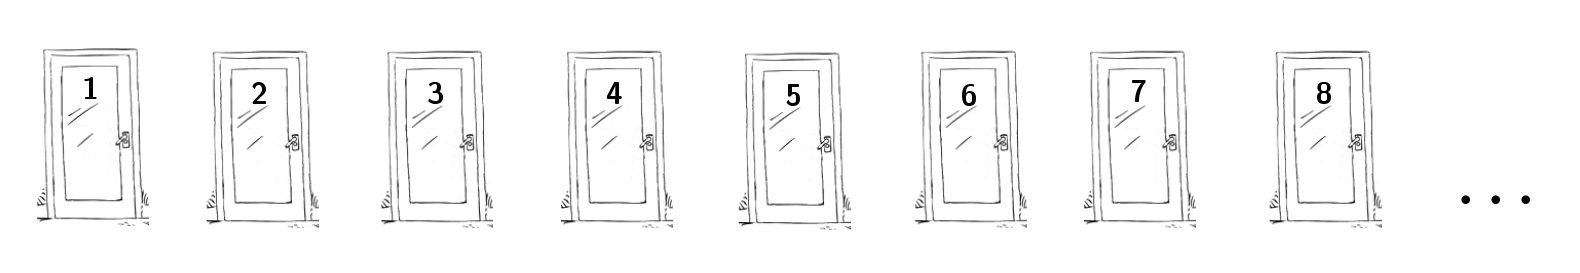
\includegraphics[scale=1.2]{door1}
\end{center}

\begin{enumerate}
\item Переселим туриста из 1 номера во 2 номер, туриста из 2 номера в 3 номер, туриста из 3 номера в 4 номер и так далее. В итоге освободится место для еще одного туриста.

\begin{center}
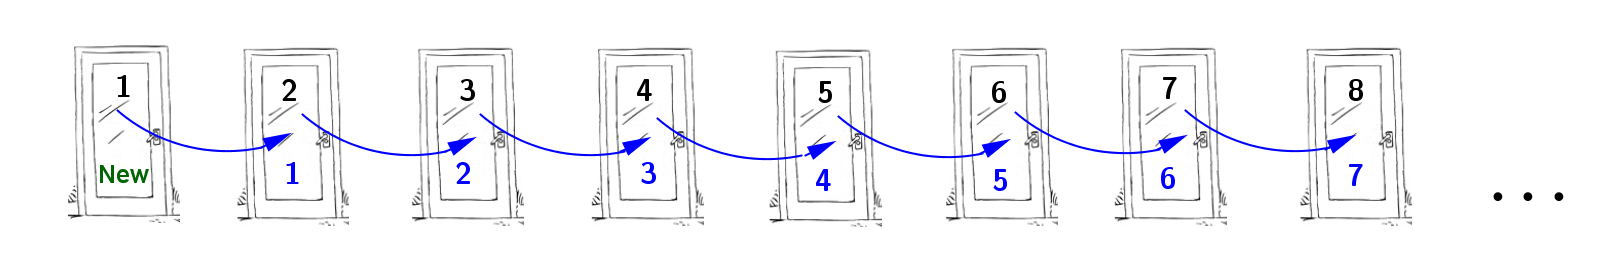
\includegraphics[scale=1.2]{door2}
\end{center}

\item Переселим туриста из 1 номера во 2 номер, из 2 номера в 4 номер, из 3 номера в 6 номер, из 4 номера в 8 номер, из 5 номера в 10 номер и так далее. В итоге освободится счётное количество номеров для дополнительного счётного количества туристов.

\begin{center}
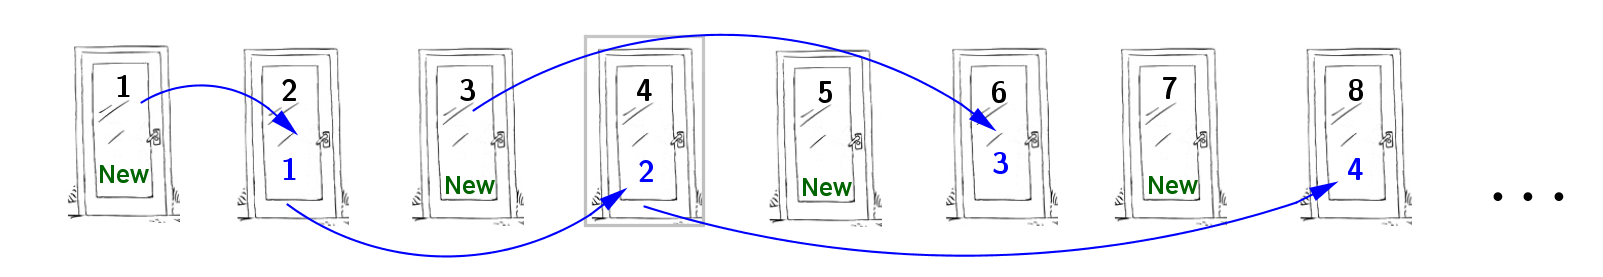
\includegraphics[scale=1.2]{door3}
\end{center}

\end{enumerate}

При решении задачи мы неявно оперировали тем фактом, что если из счётного множества удалить конечное или счётное множество, то исходное множество останется счётным. Если в счётное множество добавить конечное или счётное множество, то новое множество снова будет счётным. Чтобы доказать это достаточно построить взаимно-однозначные соответствия по аналогии с тем, как мы сделали это с жильцами.

\end{solution}
\begin{solution}{1.2}
Сопоставим каждой последовательности из нулей и единиц элемент списка $A$. Если в данный элемент списка входит  натуральное число $n$, то будем ставить в последовательности на месте $n$ единицу.

 \begin{center}
\definecolor{qqqqff}{rgb}{0.,0.,1.}
\definecolor{qqttcc}{rgb}{0.,0.2,0.8}
\definecolor{qqqqcc}{rgb}{0.,0.,0.8}
\begin{tikzpicture}[line cap=round,line join=round,>=triangle 45,x=1cm,y=1cm]
\clip(-0.7941728581796409,-2.9900066347568117) rectangle (10.560863242043467,3.5563131098557585);
\draw [rotate around={90.:(2.,0.)},line width=1.6pt,color=qqqqcc] (2.,0.) ellipse (2.7489679841754673cm and 1.8859546595880108cm);
\draw [rotate around={90.:(8,0.)},line width=1.6pt,color=qqttcc] (8,0.) ellipse (2.7489679841754686cm and 1.885954659588012cm);
\draw [->] (2.,1.5) -- (7.5,1.5);
\draw [->,line width=0.4pt] (7.5,1.5) -- (2.,1.5);
\draw [->,line width=0.4pt] (2.,0.5) -- (7.5,0.5);
\draw [->,line width=0.4pt] (7.5,0.5) -- (2.,0.5);
\draw [->,line width=0.4pt] (2.,-0.5) -- (7.5,-0.5);
\draw [->,line width=0.4pt] (7.5,-0.5) -- (2.,-0.5);
\draw [->,line width=0.4pt] (2.,-1.5) -- (7.5,-1.5);
\draw [->,line width=0.4pt] (7.5,-1.5) -- (2.,-1.5);
\draw (1.1,1.9803472454119917) node[anchor=north west] {$\mathbf{\varnothing}$};
\draw (0.9,0.9835825106355921) node[anchor=north west] {$\mathbf{\{1\}}$};
\draw (0.7,-0.04012181156719667) node[anchor=north west] {$\mathbf{\{1,3\}}$};
\draw (0.7,-1.009946958917207) node[anchor=north west] {$\mathbf{\{2,4\}}$};
\draw (7.5,1.966877451698797) node[anchor=north west] {\small{$\mathbf{00000\ldots}$}};
\draw (7.5,0.9701127169223975) node[anchor=north west] {\small{$\mathbf{10000\ldots}$}};
\draw (7.5,-0.02665201785400208) node[anchor=north west] {\small{$\mathbf{10100\ldots}$}};
\draw (7.5,-1.0503563400567908) node[anchor=north west] {\small{$\mathbf{01010\ldots}$}};
\draw (7.7,-1.8) node[anchor=north west] {$\dots$};
\draw (1.7,-1.8) node[anchor=north west] {$\dots$};
\begin{scriptsize}
\draw [fill=qqqqff] (2.,1.5) circle (2.0pt);
\draw [fill=qqqqff] (2.,0.5) circle (2.0pt);
\draw [fill=qqqqff] (2.,-0.5) circle (2.0pt);
\draw [fill=qqqqff] (2.,-1.5) circle (2.0pt);
\draw [fill=qqqqff] (7.5,1.5) circle (2.0pt);
\draw [fill=qqqqff] (7.5,0.5) circle (2.0pt);
\draw [fill=qqqqff] (7.5,-0.5) circle (2.0pt);
\draw [fill=qqqqff] (7.5,-1.5) circle (2.0pt);
\end{scriptsize}
\end{tikzpicture}
\end{center}

Таким образом каждой последовательности будет соответствовать единственный элемент списка. Множества $A$ b $S$ равномощны.

Так как мощность списка из подмножеств множества больше мощности множества и $|A|=|S|$, то $|\NN|<|S|$.
\end{solution}
\begin{solution}{1.3}
Нет! От противного, допустим $S$ существует. Для каждого $s\in S$ существует множество $A_{s}$ соответствующей мощности. Построим множество $A=\cup_{s}A_{s}$. Здесь используется аксиома выбора. И теперь построим множество $B=2^{A}$. Оно больше любого из $A_{s}$! Значит оно не было упомянуто в списке $S$.
\end{solution}
\begin{solution}{1.4}
Нет. Пусть $S$ --- множество всех последовательностей из нулей и единиц. $A = \NN \times \NN \times \NN \times \ldots$ --- декартово произведение счетного количества счетных множеств.

Тогда мощность множества $S$ точно не больше мощности множества $A$, так как в множестве $A$ существует подмножество последовательностей, состоящих только из нулей и единиц, для которого можно построить взаимно-однозначное соответствие с $S$.

Значит множеству $S$ поставлено во взаимно-однозначное соответствие подмножество $A$ и $|A| \ge |S|$.

В свою очередь мощность множества $A$ точно не больше мощности множества $S$. Построим следующее взаимно-однозначное соответствие.

\begin{center}
\definecolor{qqqqff}{rgb}{0.,0.,1.}
\definecolor{qqttcc}{rgb}{0.,0.2,0.8}
\definecolor{qqqqcc}{rgb}{0.,0.,0.8}
\begin{tikzpicture}[line cap=round,line join=round,>=triangle 45,x=1cm,y=1cm]
\clip(-0.7941728581796409,-2.9900066347568117) rectangle (10.560863242043467,3.5563131098557585);
\draw [rotate around={90.:(2.,0.)},line width=1.6pt,color=qqqqcc] (2.,0.) ellipse (2.7489679841754673cm and 1.8859546595880108cm);
\draw [rotate around={90.:(8,0.)},line width=1.6pt,color=qqttcc] (8,0.) ellipse (2.7489679841754686cm and 1.885954659588012cm);
\draw [->] (2.,1.5) -- (7.5,1.5);
\draw [->,line width=0.4pt] (7.5,1.5) -- (2.,1.5);
\draw [->,line width=0.4pt] (2.,0.5) -- (7.5,0.5);
\draw [->,line width=0.4pt] (7.5,0.5) -- (2.,0.5);
\draw [->,line width=0.4pt] (2.,-0.5) -- (7.5,-0.5);
\draw [->,line width=0.4pt] (7.5,-0.5) -- (2.,-0.5);
\draw [->,line width=0.4pt] (2.,-1.5) -- (7.5,-1.5);
\draw [->,line width=0.4pt] (7.5,-1.5) -- (2.,-1.5);
\draw (1.5,1.9803472454119917) node[anchor=north west] {$\mathbf{1}$};
\draw (1.5,0.9835825106355921) node[anchor=north west] {$\mathbf{2}$};
\draw (1.5,-0.04012181156719667) node[anchor=north west] {$\mathbf{3}$};
\draw (1.5,-1.009946958917207) node[anchor=north west] {$\mathbf{4}$};
\draw (7.5,1.966877451698797) node[anchor=north west] {\small{$\mathbf{10}$}};
\draw (7.5,0.9701127169223975) node[anchor=north west] {\small{$\mathbf{110}$}};
\draw (7.5,-0.02665201785400208) node[anchor=north west] {\small{$\mathbf{1110}$}};
\draw (7.5,-1.0503563400567908) node[anchor=north west] {\small{$\mathbf{11110}$}};
\draw (7.7,-1.8) node[anchor=north west] {$\dots$};
\draw (1.7,-1.8) node[anchor=north west] {$\dots$};
\begin{scriptsize}
\draw [fill=qqqqff] (2.,1.5) circle (2.0pt);
\draw [fill=qqqqff] (2.,0.5) circle (2.0pt);
\draw [fill=qqqqff] (2.,-0.5) circle (2.0pt);
\draw [fill=qqqqff] (2.,-1.5) circle (2.0pt);
\draw [fill=qqqqff] (7.5,1.5) circle (2.0pt);
\draw [fill=qqqqff] (7.5,0.5) circle (2.0pt);
\draw [fill=qqqqff] (7.5,-0.5) circle (2.0pt);
\draw [fill=qqqqff] (7.5,-1.5) circle (2.0pt);
\end{scriptsize}
\end{tikzpicture}
\end{center}

Тогда, например, элементу $(1,2,2,3,\ldots) \in A$ будет соответствовать элемент $101101101110\ldots$. Каким бы ни был элемент из множества $A$, в последовательности никогда не будет двух нулей подряд. Значит множеству $A$ поставлено во взаимно-однозначное соответствие какое-то подмножество $S$ и $|A| \le |S|$.

Так как $|A| \ge |S|$ и $|A| \le |S|$, мощности множеств совпадают, $|A|=|S|$. Оба множества имеют мощность континуум.

При решении этой задачи можно просто привести следующий контр-пример. Бесконечные вправо последовательности из 0 и 1 --- это декартово произведение счётного количества $A_{i}$, где каждое $A_{i}=\{0,1\}$
\end{solution}
\begin{solution}{1.5}
Для того, чтобы каждому элементу из множества $(0;1) \times (0;1)$ поставить единственным образом в соответствие элемент из $\RR^{2}$ нужно найти такое отображение, что:
\[ \lim_{x \to 0} f(x) = - \infty \text{ и } \lim_{x \to 1} f(x) = + \infty.\] Аналогичное отображение нужно подобрать для переменной $y$. Первое, что приходит в голову --- начать экспериментировать с экспонентами и тангенсами, но это плохая идея.

Попробуем не заморачиваться. Чтобы $\lim_{x \to 0} f(x) = - \infty$ достаточно взять функцию $-\dfrac{1}{x^2}$. Чтобы получить  $\lim_{x \to 1} f(x) = + \infty$ достаточно взять функцию $\dfrac{1}{(x-1)^2}$. Тогда для функции $-\dfrac{1}{x^2} + \dfrac{1}{(x-1)^2}$ получаем:

\[\lim_{x \to 0} \left(-\frac{1}{x^2} + \dfrac{1}{(x-1)^2}\right) = -\infty -1 = -\infty,\]

\[\lim_{x \to 1} \left(-\frac{1}{x^2} + \dfrac{1}{(x-1)^2}\right) = -1 + \infty = +\infty,\].

Таким образом по правилу $(x,y) \leftrightarrow \left(-\dfrac{1}{x^2} + \dfrac{1}{(x-1)^2},-\dfrac{1}{y^2} + \dfrac{1}{(y-1)^2}\right)$ мы каждому элементу из $(0;1) \times (0;1)$ поставим в соответствие элемент из $\RR^{2}$.

Для того, чтобы доказать, что множества $[0;1] \times [0;1]$ и $\RR^{2}$ равномощны, нам нужно построить взаимно-однозначное соответствие между этими двумя множествами.

\begin{center}
\definecolor{qqqqff}{rgb}{0.,0.,1.}
\definecolor{qqwuqq}{rgb}{0.,0.39215686274509803,0.}
\definecolor{ffqqqq}{rgb}{1.,0.,0.}
\begin{tikzpicture}[line cap=round,line join=round,>=triangle 45,x=0.8cm,y=0.8cm]
\clip(-4.111289704910403,-1.5128932941321722) rectangle (10.605912648926926,6.79873266366131);
\fill[line width=1.6pt,color=qqwuqq,fill=qqwuqq,fill opacity=0.1] (0.,4.) -- (0.,1.) -- (-3.,1.) -- (-3.,4.) -- cycle;
\fill[color=qqqqff,fill=qqqqff,fill opacity=0.1] (5.94,5.76) -- (4.66,5.58) -- (3.4,5.16) -- (3.06,4.02) -- (3.06,2.74) -- (2.94,1.7) -- (3.,0.82) -- (3.46,-0.18) -- (4.18,-0.74) -- (5.4,-0.84) -- (6.96,-0.9) -- (7.98,-0.42) -- (8.7,0.5) -- (9.18,1.76) -- (9.4,3.16) -- (9.18,4.4) -- (8.58,5.26) -- (7.58,5.7) -- (6.5,5.72) -- cycle;
\draw [line width=1.6pt,color=qqwuqq] (0.,4.)-- (0.,1.);
\draw [line width=1.6pt,color=qqwuqq] (0.,1.)-- (-3.,1.);
\draw [line width=1.6pt,color=qqwuqq] (-3.,1.)-- (-3.,4.);
\draw [line width=1.6pt,color=qqwuqq] (-3.,4.)-- (0.,4.);
\draw [line width=1.6pt,dash pattern=on 8pt off 8pt,color=qqqqff] (6.059421412128413,5.75334642883689)-- (6.06,-0.84);
\draw (-3.1,3.0178802542890866) node[anchor=north west] {$\mathbf{[0;1] \times [0;1]}$};
\draw (3.9816092539937755,2.142972258731878) node[anchor=north west] {$\mathbf{\RR^2}$};
\draw [->,line width=0.4pt,color=qqwuqq] (-3.,4.) -- (0.015114492880381025,3.969771014239238);
\draw [->,line width=0.4pt,color=qqwuqq] (0.015114492880381183,0.9697710142392378) -- (0.015114492880381185,3.969771014239238);
\begin{scriptsize}
\draw [fill=ffqqqq] (0.,4.) circle (2.5pt);
\end{scriptsize}
\end{tikzpicture}
\end{center}

В предыдущем пункте задачи мы нашли отображение, которое переводит все точки квадрата в точки плоскости, но при этом мы не нашли ни одной точки, которой в соответствие можно было бы поставить границу квадрата. Возьмем на плоскости произвольную прямую. Прямая равномощна полупрямой с выколотым началом. То есть между ними можно установить взаимно-однозначное соответствие.

\begin{center}
\definecolor{wwqqzz}{rgb}{0.4,0.,0.6}
\definecolor{qqqqff}{rgb}{0.,0.,1.}
\definecolor{qqwuqq}{rgb}{0.,0.39215686274509803,0.}
\definecolor{ffqqqq}{rgb}{1.,0.,0.}
\begin{tikzpicture}[line cap=round,line join=round,>=triangle 45,x=0.8cm,y=0.8cm]
\clip(-3.525776137780285,-1.4871732097146722) rectangle (11.158053875118634,6.026209026184774);
\fill[line width=1.6pt,color=qqwuqq,fill=qqwuqq,fill opacity=0.1] (0.,4.) -- (0.,1.) -- (-3.,1.) -- (-3.,4.) -- cycle;
\fill[color=qqqqff,fill=qqqqff,fill opacity=0.1] (5.94,5.76) -- (4.66,5.58) -- (3.4,5.16) -- (3.06,4.02) -- (3.06,2.74) -- (2.94,1.7) -- (3.,0.82) -- (3.46,-0.18) -- (4.18,-0.74) -- (5.4,-0.84) -- (6.96,-0.9) -- (7.98,-0.42) -- (8.7,0.5) -- (9.18,1.76) -- (9.4,3.16) -- (9.18,4.4) -- (8.58,5.26) -- (7.58,5.7) -- (6.5,5.72) -- cycle;
\draw [line width=1.6pt,color=qqwuqq] (0.,4.)-- (0.,1.);
\draw [line width=1.6pt,color=qqwuqq] (0.,1.)-- (-3.,1.);
\draw [line width=1.6pt,color=qqwuqq] (-3.,1.)-- (-3.,4.);
\draw [line width=1.6pt,color=qqwuqq] (-3.,4.)-- (0.,4.);
\draw (-3.1,3.0178802542890866) node[anchor=north west] {$\mathbf{[0;1] \times [0;1]}$};
\draw (3.9816092539937755,2.142972258731878) node[anchor=north west] {$\mathbf{\RR^2}$};
\draw [line width=1.6pt,dotted,color=wwqqzz] (5.9813989581245375,2.04923211635075)-- (5.9813989581245375,5.673850955087756);
\draw [->,line width=1.6pt,dash pattern=on 8pt off 8pt,color=qqqqff] (6.012485672022963,-0.8729189901012959) -- (5.981398958124537,2.049232116350843);
\draw [->,line width=0.4pt,color=qqwuqq] (-3.,4.) -- (0.015114492880381025,3.969771014239238);
\draw [->,line width=0.4pt,color=qqwuqq] (0.015114492880381183,0.9697710142392378) -- (0.015114492880381185,3.969771014239238);
\begin{scriptsize}
\draw [fill=ffqqqq] (0.,4.) circle (2.5pt);
\end{scriptsize}
\end{tikzpicture}
\end{center}

Любой интервал равномощен полупрямой. Сопоставим между собой границу квадрата и незанятую полупрямую с включённым началом.

\begin{center}
\definecolor{qqqqff}{rgb}{0.,0.,1.}
\definecolor{qqwuqq}{rgb}{0.,0.39215686274509803,0.}
\definecolor{ffqqqq}{rgb}{1.,0.,0.}
\begin{tikzpicture}[line cap=round,line join=round,>=triangle 45,x=0.8cm,y=0.8cm]
\clip(-3.579776155240749,-1.1806060881890135) rectangle (9.949582062279424,5.964416424276412);
\fill[line width=1.6pt,color=qqwuqq,fill=qqwuqq,fill opacity=0.1] (0.015114492880381185,3.969771014239238) -- (0.015114492880381185,0.969771014239238) -- (-3.,1.) -- (-3.,4.) -- cycle;
\fill[color=qqqqff,fill=qqqqff,fill opacity=0.1] (5.94,5.76) -- (4.66,5.58) -- (3.4,5.16) -- (3.06,4.02) -- (3.06,2.74) -- (2.94,1.7) -- (3.,0.82) -- (3.46,-0.18) -- (4.18,-0.74) -- (5.4,-0.84) -- (6.96,-0.9) -- (7.98,-0.42) -- (8.7,0.5) -- (9.18,1.76) -- (9.4,3.16) -- (9.18,4.4) -- (8.58,5.26) -- (7.58,5.7) -- (6.5,5.72) -- cycle;
\draw [line width=1.6pt,color=qqwuqq] (0.015114492880381185,3.969771014239238)-- (0.015114492880381185,0.969771014239238);
\draw [line width=1.6pt,color=qqwuqq] (0.015114492880381185,0.969771014239238)-- (-3.,1.);
\draw [line width=1.6pt,color=qqwuqq] (-3.,1.)-- (-3.,4.);
\draw [line width=1.6pt,color=qqwuqq] (-3.,4.)-- (0.015114492880381185,3.969771014239238);
\draw (-3.1,3.0178802542890866) node[anchor=north west] {$\mathbf{[0;1] \times [0;1]}$};
\draw (3.9816092539937755,2.142972258731878) node[anchor=north west] {$\mathbf{\RR^2}$};
\draw [->,line width=1.6pt,dash pattern=on 7pt off 7pt,color=qqqqff] (6.012485672022963,-0.8729189901012959) -- (5.981398958124537,2.049232116350843);
\draw [->,line width=0.4pt,color=qqwuqq] (-3.,4.) -- (0.015114492880381025,3.969771014239238);
\draw [->,line width=0.4pt,color=qqwuqq] (0.015114492880381183,0.9697710142392378) -- (0.015114492880381185,3.969771014239238);
\draw [->,line width=1.6pt,color=qqwuqq] (5.98314370935182,5.7470773364447645) -- (6.,2.);
\begin{scriptsize}
\draw [fill=ffqqqq] (0.015114492880381185,3.969771014239238) circle (2.5pt);
\draw [fill=ffqqqq] (6.,2.) circle (2.5pt);
\end{scriptsize}
\end{tikzpicture}
\end{center}

Проделав всё это мы сопоставили плоскости квадрат с его границей. Заметим, что, используя это отображение, можно доказать равномощность $[0;1]$ и $\RR$.

\end{solution}
\begin{solution}{1.6}
Да, это верно. Пусть точка $a$ --- изолированная точка некоторого множества A. Условие существования такой окрестности точки $a$, для~которой выполнено следующее равенство $U(a) \cap A = a$ эквивалентно тому, что для~любой окрестности точки $a$ верно, что $U(a) \cap A \ne \varnothing $, так как каким угодно интервалом точку $a$ не~накрой, то для~любой окрестности точки $a$ её пересечение с множеством $A$ будет как минимум давать точку $a$ то есть не~будет пустым. Так же это условие эквивалентно тому, что для~любой окрестности точки $a$ верно, что $U(a) \cap (\RR \setminus A)\ne \varnothing$. Это следует из~того что, если существует окрестность, для которой её пересечение с множеством A~даст точку $a$, то при удалении точки $a$ получим, что пересечение проколотой окрестности точки $a$ с~множеством A даёт пустое множество. То есть имеет место не пустое пересечение с частью множества $\RR \setminus A$. Дальнейшие попытки уменьшить или увеличить исходную окрестность не~приведут к~иному результату, что и завершает решение задачи.
\end{solution}
\begin{solution}{1.7}
Выберем $\dt_1=1$. Выберем в~$\dot U_{\dt_1} (a)$ точку $a_1 \in A$. Положим $\dt_2 = \min (\frac{1}{2}, |a_1 - a|)$. Теперь в $\dot U_{\dt_2} (a)$ выберем точку $a_2 \in A$. Очевидно, что $a_1 \ne a_2$. Далее положим $\dt_3 = \min (\frac{1}{3}, |a_2 - a|)$, рассмотрим $\dot U_{dt_3} (a)$ и т.д. На~шаге с~номером $n$ получается точка $a_n \in A$, отличная от~предыдущих точек. Неограниченное продолжение этого процесса даёт искомое бесконечное множество.
\end{solution}
\begin{solution}{1.8}

\end{solution}
\begin{solution}{1.9}
Предположим, что это верно. Тогда существуют два открытых непересекающихся и непустых множества $A$ и $B$, которые в~объединении дают всё множество действительных чисел. Рассмотрим множество $A$. Оно непусто и открыто. Тогда дополнением к~нему будет являться множество $B$, которое по~определению будет замкнутым. Получается, что $B$ одновременно и открыто, и замкнуто, и не пусто, и не всё множество действительных чисел (так как множество $A$ непусто). Получаем противоречие с задачей \ref{resh_1}.

Аналогичные рассуждения применяем для~случая двух замкнутых множеств.
\end{solution}
\begin{solution}{1.10}
Множество $\{\frac{1}{n}\}_{n=1}^{\infty} \cup \{0\}$ является компактом. Так как точка $0$ является предельной точкой для множества  $\{\frac{1}{n}\}_{n=1}^{\infty}$, то какой бы окрестностью мы точку ноль не покрыли (а мы её обязаны покрыть) за~пределами этой окрестности останется лишь конечное число точек исходного множества, которое мы можем покрыть конечным числом интервалов. Получается, что из всякого покрытия открытыми множествами этого множества можно выделить конечное подпокрытие. Это и соответствует определению компакта.

Множество точек  $\{\frac{1}{n}\}_{n=1}^{\infty}$ не является компактом. Достаточно предъявить покрытие $\cup_{n=1}^{\infty} \left(\frac{1}{n} - \frac{1}{10^n}; \frac{1}{n} + \frac{1}{10^n}\right)$.
Из~данного покрытия нельзя выделить конечное подпокрытие (попробовать выделить самостоятельно), а это противоречит определению компакта.
\end{solution}
\begin{solution}{1.11}
Да, правда!
\end{solution}
\begin{solution}{1.12}
Конечно да! Радиус --- это линейная функция от длины окружности, а линейная функция равномерно непрерывна.

\[l = 2 \pi r \Rightarrow r = \frac{1}{2 \pi} l \]

Равномерная непрерывность означает, что при какой бы длине окружности мы не увеличивали радиус, прирост длины окружности будет одним и тем же. Прирост функции зависит только от прироста аргумента.

\[r_1 - r_2 = \frac{1}{2\pi} (l_1 - l_2) \]

Оба раза $l_1 - l_2 = 1$, значит в обоих ситуациях радиус увеличится на $r_1 - r_2 = \dfrac{1}{2\pi}$. Что в случае с апельсином, что в случае с Землей, зазор между лентой и поверхностью будет одинаковым, и кот Саймона без труда пролезет между ленточкой и Землей.
\end{solution}
\begin{solution}{1.13}
\end{solution}
\begin{solution}{1.14}
\end{solution}
\begin{solution}{1.15}
Спросите у~Google или Yandex «Что такое функция Римана?»
\end{solution}
\begin{solution}{1.16}
 Да, обязательно. Рассмотрим первые 50 сапог. Если среди них левых и правых поровну, то ничего больше делать не надо. Если не поровну, пусть, для определённости, правых сапог больше. Для каждых 50 подряд стоящих сапог рассмотрим разность между числом правых и левых сапог. По нашему предположению для первых 50 сапог эта разность положительна. Очевидно, что для последних 50 сапогов эта разность отрицательна, так как в противном случае правых и левых сапог было бы не поровну. Теперь задумаемся, как меняется разность при сдвиге на 1 сапог. Также заметим, что разница для первых 50 сапог чётна, так как либо не может быть такого, что одних чётное количество, а других нечётное. Поскольку добавляется один сапог и исчезает тоже один, то разность или не меняется, или меняется на 2. Осталось применить нечто вроде теоремы о промежуточном значении.
\end{solution}
\begin{solution}{1.17}
Да, это верно! Пусть $M$ --- бесконечное множество. Удалим из него счётные множества $B$ и $A$. Тогда с одной стороны $N = (M\setminus A)\setminus B \Rightarrow (M \setminus A) = N \cap B $. С другой стороны $N = M \setminus (B \cup A) \Rightarrow M = N \cap (A \cap B)$. Установим между множествами $M\setminus A$ и $M$ взаимно-однозначное соответствие.

Если $x \in N$, то во множестве  $M\setminus A$ он будет соответствовать самому себе. Если же $x \in A \cap B$, то учитывая что множества $A$ и $B$ счётные, то их объединение тоже является счётным множество и можно установить взаимно-однозначное соответствие между $A \cap B$ и $B$. Таким образом каждому элементу из $M\setminus A$ соответствует единственный элемент из $M$.
\end{solution}
\begin{solution}{1.18}
Нет! Это враньё! Множество иррациональных чисел можно получить, выбросив из множества действительных чисел все рациональные. Полученное множество равномощно исходному.
\end{solution}
\begin{solution}{1.19}
$|A| <|B|$
\end{solution}
\begin{solution}{1.20}
Да. Все элементы этого множества можно пересчитать змейкой.
\end{solution}
\begin{solution}{1.21}

Да, это чистая правда в обоих случаях. Множество всех последовательностей натуральных чисел --- это ни что иное, как декартово произведение счётного числа счётных множеств. Это означает, что множество последовательностей натуральных чисел имеет мощность континуум.

Множество всех вещественных числовых последовательностей совпадает с декартовым произведением $\RR \times \RR \times \RR \times \ldots$
\end{solution}
\begin{solution}{1.22}
Субмарина начинает свое движение из неизвестной нам точки и движется с постоянной скоростью. Нанесем все возможные комбинации (начало движения, скорость) на плоскость.

Тогда если субмарина движется со скоростью $2$ и начинает движение из точки $-4$ мы можем уничтожить ее несколькими способами. Выстрелив в точку $-4$  в нулевую минуту, в точку $-2$ в первую минуту, в точку $0$ во вторую минуту и так далее.

Аналогично для любой другой точки старта субмарины. Перечислим все возможные комбинации $(\text{старт},\text{скорость})$ и нанесём их на плоскость.

\begin{center}
\definecolor{ffqqqq}{rgb}{1.,0.,0.}
\definecolor{qqqqff}{rgb}{0.,0.,1.}
\definecolor{cqcqcq}{rgb}{0.7529411764705882,0.7529411764705882,0.7529411764705882}
\begin{tikzpicture}[line cap=round,line join=round,>=triangle 45,x=0.8cm,y=0.8cm]
\draw[->,color=black] (-6.92,0.) -- (8.5,0.);
\foreach \x in {-6.,-5.,-4.,-3.,-2.,-1.,1.,2.,3.,4.,5.,6.,7.,8.}
\draw[shift={(\x,0)},color=black] (0pt,2pt) -- (0pt,-2pt) node[below] {\footnotesize $\x$};
\draw[->,color=black] (0.,-3.72) -- (0.,4.82);
\foreach \y in {-3.,-2.,-1.,1.,2.,3.,4.}
\draw[shift={(0,\y)},color=black] (2pt,0pt) -- (-2pt,0pt) node[left] {\footnotesize $\y$};
\draw[color=black] (0pt,-10pt) node[right] {\footnotesize $0$};
\clip(-6.92,-3.72) rectangle (8.5,4.82);
\draw (3.9,-0.4) node[anchor=north west] {\small{$ \text{Точка, из которой} $}};
\draw (0.3,4.76) node[anchor=north west] {\parbox{3.56 cm}{\small{$ \text{Скорость } \\ \text{субмарины} $}}};
\draw (3.5,-1.04) node[anchor=north west] {\small{$\text{стартовала субмарина}$}};
\draw [->,color=ffqqqq] (0.,0.) -- (1.,0.);
\draw [->,color=ffqqqq] (1.,0.) -- (1.,1.);
\draw [->,color=ffqqqq] (1.,1.) -- (0.,1.);
\draw [->,color=ffqqqq] (0.,1.) -- (-1.,1.);
\draw [->,color=ffqqqq] (-1.,1.) -- (-1.,0.);
\draw [->,color=ffqqqq] (-1.,0.) -- (-1.,-1.);
\draw [->,color=ffqqqq] (-1.,-1.) -- (0.,-1.);
\draw [->,color=ffqqqq] (0.,-1.) -- (1.,-1.);
\draw [->,color=ffqqqq] (1.,-1.) -- (2.,-1.);
\draw [->,color=ffqqqq] (2.,-1.) -- (2.,0.);
\draw [->,color=ffqqqq] (2.,0.) -- (2.,1.);
\draw [->,color=ffqqqq] (2.,1.) -- (2.,2.);
\draw [->,color=ffqqqq] (2.,2.) -- (1.,2.);
\draw [->,color=ffqqqq] (1.,2.) -- (0.,2.);
\draw [->,color=ffqqqq] (0.,2.) -- (-1.,2.);
\draw [->,color=ffqqqq] (-1.,2.) -- (-2.,2.);
\draw [->,color=ffqqqq] (-2.,2.) -- (-2.,1.);
\draw [->,color=ffqqqq] (-2.,1.) -- (-2.,0.);
\draw [->,color=ffqqqq] (-2.,0.) -- (-2.,-1.);
\draw [->,color=ffqqqq] (-2.,-1.) -- (-2.,-2.);
\draw [->,color=ffqqqq] (-2.,-2.) -- (-1.,-2.);
\draw [->,color=ffqqqq] (-1.,-2.) -- (0.,-2.);
\draw [->,color=ffqqqq] (0.,-2.) -- (1.,-2.);
\draw [->,color=ffqqqq] (1.,-2.) -- (2.,-2.);
\draw [->,color=ffqqqq] (2.,-2.) -- (3.,-2.);
\draw [->,color=ffqqqq] (3.,-2.) -- (3.,-1.);
\draw [->,color=ffqqqq] (3.,-1.) -- (3.,0.);
\draw [->,color=ffqqqq] (3.,0.) -- (3.,1.);
\draw [->,color=ffqqqq] (3.,1.) -- (3.,2.);
\draw [->,color=ffqqqq] (3.,2.) -- (3.,3.);
\draw [->,color=ffqqqq] (3.,3.) -- (2.,3.);
\draw [->,color=ffqqqq] (2.,3.) -- (1.,3.);
\draw [->,color=ffqqqq] (1.,3.) -- (0.,3.);
\draw [->,color=ffqqqq] (0.,3.) -- (-1.,3.);
\draw [->,color=ffqqqq] (-1.,3.) -- (-2.,3.);
\draw [->,color=ffqqqq] (-2.,3.) -- (-3.,3.);
\draw [->,color=ffqqqq] (-3.,3.) -- (-3.,2.);
\draw [->,color=ffqqqq] (-3.,2.) -- (-3.,1.);
\draw [->,color=ffqqqq] (-3.,1.) -- (-3.,0.);
\draw [->,color=ffqqqq] (-3.,0.) -- (-3.,-1.);
\draw [->,color=ffqqqq] (-3.,-1.) -- (-3.,-2.);
\draw [->,color=ffqqqq] (-3.,-2.) -- (-3.,-3.);
\draw [->,color=ffqqqq] (-3.,-3.) -- (-2.,-3.);
\draw [->,color=ffqqqq] (-2.,-3.) -- (-1.,-3.);
\draw [->,color=ffqqqq] (-1.,-3.) -- (0.,-3.);
\draw [->,color=ffqqqq] (0.,-3.) -- (1.,-3.);
\draw (1.34,-3) node[anchor=north west] {$\mathbf{\dots}$};
\begin{scriptsize}
\draw [fill=qqqqff] (1.,2.) circle (2.5pt);
\draw [fill=qqqqff] (2.,2.) circle (2.5pt);
\draw [fill=qqqqff] (2.,1.) circle (2.5pt);
\draw [fill=qqqqff] (3.,1.) circle (2.5pt);
\draw [fill=qqqqff] (1.,1.) circle (2.5pt);
\draw [fill=qqqqff] (0.,1.) circle (2.5pt);
\draw [fill=qqqqff] (-1.,1.) circle (2.5pt);
\draw [fill=qqqqff] (-1.,2.) circle (2.5pt);
\draw [fill=qqqqff] (-2.,2.) circle (2.5pt);
\draw [fill=qqqqff] (-3.,2.) circle (2.5pt);
\draw [fill=qqqqff] (3.,2.) circle (2.5pt);
\draw [fill=qqqqff] (-3.,1.) circle (2.5pt);
\draw [fill=qqqqff] (-2.,1.) circle (2.5pt);
\draw [fill=qqqqff] (-3.,0.) circle (2.5pt);
\draw [fill=qqqqff] (0.,2.) circle (2.5pt);
\draw [fill=qqqqff] (-2.,0.) circle (2.5pt);
\draw [fill=qqqqff] (-1.,0.) circle (2.5pt);
\draw [fill=qqqqff] (0.,0.) circle (2.5pt);
\draw [fill=qqqqff] (1.,0.) circle (2.5pt);
\draw [fill=qqqqff] (2.,0.) circle (2.5pt);
\draw [fill=qqqqff] (3.,0.) circle (2.5pt);
\draw [fill=qqqqff] (3.,-1.) circle (2.5pt);
\draw [fill=qqqqff] (3.,-2.) circle (2.5pt);
\draw [fill=qqqqff] (2.,-2.) circle (2.5pt);
\draw [fill=qqqqff] (2.,-1.) circle (2.5pt);
\draw [fill=qqqqff] (1.,-1.) circle (2.5pt);
\draw [fill=qqqqff] (1.,-2.) circle (2.5pt);
\draw [fill=qqqqff] (0.,-2.) circle (2.5pt);
\draw [fill=qqqqff] (-1.,-2.) circle (2.5pt);
\draw [fill=qqqqff] (-1.,-1.) circle (2.5pt);
\draw [fill=qqqqff] (0.,-1.) circle (2.5pt);
\draw [fill=qqqqff] (-2.,-1.) circle (2.5pt);
\draw [fill=qqqqff] (-3.,-1.) circle (2.5pt);
\draw [fill=qqqqff] (-3.,-2.) circle (2.5pt);
\draw [fill=qqqqff] (-2.,-2.) circle (2.5pt);
\draw [fill=qqqqff] (3.,3.) circle (2.5pt);
\draw [fill=qqqqff] (2.,3.) circle (2.5pt);
\draw [fill=qqqqff] (1.,3.) circle (2.5pt);
\draw [fill=qqqqff] (0.,3.) circle (2.5pt);
\draw [fill=qqqqff] (-1.,3.) circle (2.5pt);
\draw [fill=qqqqff] (-2.,3.) circle (2.5pt);
\draw [fill=qqqqff] (-3.,3.) circle (2.5pt);
\draw [fill=qqqqff] (-3.,-3.) circle (2.5pt);
\draw [fill=qqqqff] (-2.,-3.) circle (2.5pt);
\draw [fill=qqqqff] (-1.,-3.) circle (2.5pt);
\draw [fill=qqqqff] (0.,-3.) circle (2.5pt);
\draw [fill=qqqqff] (1.,-3.) circle (2.5pt);
\end{scriptsize}
\end{tikzpicture}
\end{center}

Все возможные положения субмарины представляют собой объединение счётного количества счётных множеств. Количество элементов этого объединения мы можем пересчитать змейкой.
\end{solution}
\begin{solution}{1.23}
Мощность $2^{A}$ не меньше мощности $A$, т.к. есть одноточечные подмножества, которые можно сопоставить с элементами $A$. Допустим все же, что $2^{A}$ и $A$ равномощны. Значит есть взаимно однозначное соответствие $b\longleftrightarrow B$, где $b\in A$ и $B\in 2^{A}$. Построим $C\subset A$ по принципу: будем включать туда только такие $b$, которые не входят в соответствующее $B$. Этому множеству $C$ должен соответствовать некий элемент $c$. С одной стороны $c$ не может входить в $C$, с другой стороны - обязан. Противоречие.
\end{solution}
\begin{solution}{1.24}
да
\end{solution}
\begin{solution}{1.25}
За одну операцию дарения - забирания количество конфет у детишек каждый раз будет увеличиваться на одну.

Конфета номер 1 к Новому Году окажется у Деда Мороза. Он сразу же отберет её у Вовочки.

Конфета номер 2015 к Новому Году окажется также у Деда Мороза! Рано или поздно наступит момент, когда он её у Вовочки отберет.

У Вовочки к Новому Году не будет ни одной конфеты. Дед Мороз всё оставит себе.
\end{solution}
\begin{solution}{1.26}
Множество последовательностей «похожих» на последовательность из одних нулей будет либо счетным, либо континуальным. Среди всех этих последовательностей есть такие, которые отличаются от нулевой только первой цифрой. Есть такие, которые отличаются от нулевой первой или второй цифрой, есть такие, которые отличаются первой или второй или третьей цифрой и так далее. Все такие отличия можно занумеровать.

\begin{center}
\definecolor{qqqqff}{rgb}{0.,0.,1.}
\definecolor{qqttcc}{rgb}{0.,0.2,0.8}
\definecolor{qqqqcc}{rgb}{0.,0.,0.8}
\begin{tikzpicture}[line cap=round,line join=round,>=triangle 45,x=1.0cm,y=1.0cm]
\clip(-0.4849001735617755,-3.081553672504657) rectangle (10.42080979412848,3.2409971695233946);
\draw [rotate around={90.:(2.,0.)},line width=1.6pt,color=qqqqcc] (2.,0.) ellipse (2.7489679841754673cm and 1.8859546595880108cm);
\draw [rotate around={90.:(8.,0.)},line width=1.6pt,color=qqttcc] (8.,0.) ellipse (2.7489679841754686cm and 1.885954659588012cm);
\draw [->] (2.,2.) -- (7.,2.);
\draw [->,line width=0.4pt] (7.,2.) -- (2.,2.);
\draw [->,line width=0.4pt] (2.,1.4) -- (7.,1.4);
\draw [->,line width=0.4pt] (7.,1.4) -- (2.,1.4);
\draw [->,line width=0.4pt] (2.,0.8) -- (7.,0.8);
\draw [->,line width=0.4pt] (7.,0.8) -- (2.,0.8);
\draw [->,line width=0.4pt] (2.,0.2) -- (7.,0.2);
\draw [->,line width=0.4pt] (7.,0.2) -- (2.,0.2);
\draw (1.3,2.381738880633563) node[anchor=north west] {$\mathbf{1}$};
\draw (1.3,1.7881369456833312) node[anchor=north west] {$\mathbf{2}$};
\draw (1.3,1.1945350107330993) node[anchor=north west] {$\mathbf{3}$};
\draw (1.3,0.6009330757828673) node[anchor=north west] {$\mathbf{4}$};
\draw (7.287143765437737,2.371301311340497) node[anchor=north west] {$\mathbf{1000 \ldots}$};
\draw (7.287143765437737,1.7500899840669981) node[anchor=north west] {$\mathbf{0100 \ldots}$};
\draw (7.314753157761003,1.1564880491167662) node[anchor=north west] {$\mathbf{1100 \ldots}$};
\draw (7.300948461599369,0.549081418004901) node[anchor=north west] {$\mathbf{0010 \ldots}$};
\draw [->,line width=0.4pt] (2.,-0.4) -- (7.,-0.4);
\draw [->,line width=0.4pt] (7.,-0.4) -- (2.,-0.4);
\draw (1.3,-0.07972174850936878) node[anchor=north west] {$\mathbf{5}$};
\draw (7.480409511700602,-1.9) node[anchor=north west] {$\dots$};
\draw (1.6134136430064763,-1.9) node[anchor=north west] {$\dots$};
\draw [->,line width=0.4pt] (7.,-1.) -- (2.,-1.);
\draw [->,line width=0.4pt] (7.,-1.6) -- (2.,-1.6);
\draw [->,line width=0.4pt] (2.,-1.) -- (7.,-1.);
\draw [->,line width=0.4pt] (2.,-1.6) -- (7.,-1.6);
\draw (1.3,-0.6000754902792298) node[anchor=north west] {$\mathbf{6}$};
\draw (1.3,-1.207482121391095) node[anchor=north west] {$\mathbf{7}$};
\draw (7.300948461599369,-0.04452051694533093) node[anchor=north west] {$\mathbf{0110 \ldots}$};
\draw (7.300948461599369,-0.6519271480571961) node[anchor=north west] {$\mathbf{1010 \ldots}$};
\draw (7.287143765437737,-1.2455290830074282) node[anchor=north west] {$\mathbf{1110 \ldots}$};
\begin{scriptsize}
\draw [fill=qqqqff] (2.,2.) circle (2.0pt);
\draw [fill=qqqqff] (2.,1.4) circle (2.0pt);
\draw [fill=qqqqff] (2.,0.8) circle (2.0pt);
\draw [fill=qqqqff] (2.,0.2) circle (2.0pt);
\draw [fill=qqqqff] (7.,2.) circle (2.0pt);
\draw [fill=qqqqff] (7.,1.4) circle (2.0pt);
\draw [fill=qqqqff] (7.,0.8) circle (2.0pt);
\draw [fill=qqqqff] (7.,0.2) circle (2.0pt);
\draw [fill=qqqqff] (2.,-0.4) circle (2.0pt);
\draw [fill=qqqqff] (7.,-0.4) circle (2.0pt);
\draw [fill=qqqqff] (7.,-1.) circle (2.0pt);
\draw [fill=qqqqff] (7.,-1.6) circle (2.0pt);
\draw [fill=qqqqff] (2.,-1.) circle (2.0pt);
\draw [fill=qqqqff] (2.,-1.6) circle (2.0pt);
\end{scriptsize}
\end{tikzpicture}
\end{center}

Таким образом последовательностей, отличающихся от нулевой счётное количество.

Гораздо более интересным вопросом является вопрос о количестве таких счетных классов.

\begin{center}
\definecolor{qqttcc}{rgb}{0.,0.2,0.8}
\definecolor{qqqqff}{rgb}{0.,0.,1.}
\begin{tikzpicture}[line cap=round,line join=round,>=triangle 45,x=1cm,y=1cm]
\clip(-2.5126768593015663,-2.9476257822190104) rectangle (12.312718113652455,6.872040745791953);
\draw [rotate around={0.:(4.8,1.74)}] (4.8,1.74) ellipse (5.cm and 4.cm);
\draw (6.5,-1.48)-- (5.52,-0.82)-- (5.84,-0.22)-- (6.14,-0.38)-- (6.68,0.44)-- (7.14,-0.3)-- (6.98,-1.14)-- (6.32,-1.02);
\draw (5.52,-0.82)-- (6.14,-0.38);
\draw (6.32,-1.02)-- (6.68,0.44);
\draw (6.32,-1.02)-- (7.14,-0.3);
\draw (6.98,-1.14)-- (6.14,-0.38);
\draw (6.98,-1.14)-- (6.68,0.44);
\draw (6.32,-1.02)-- (5.52,-0.82);
\draw (6.32,-1.02)-- (5.84,-0.22);
\draw (6.5,-1.48)-- (6.98,-1.14);
\draw (6.5,-1.48)-- (6.32,-1.02);
\draw (6.5,-1.48)-- (6.68,0.44);
\draw (6.32,-1.02)-- (6.14,-0.38);
\draw (7.14,-0.3)-- (6.14,-0.38);
\draw (7.14,-0.3)-- (5.52,-0.82);
\draw (7.24,2.36)-- (7.72,2.6);
\draw (7.72,2.6)-- (8.52,2.8);
\draw (8.52,2.8)-- (8.,3.);
\draw (8.,3.)-- (8.02,3.5);
\draw (8.02,3.5)-- (7.24,2.36);
\draw (7.72,2.6)-- (8.,3.);
\draw (7.72,2.6)-- (6.86,2.78);
\draw (8.52,2.8)-- (6.86,2.78);
\draw (8.,3.)-- (6.86,2.78);
\draw (8.02,3.5)-- (6.86,2.78);
\draw (7.24,2.36)-- (6.86,2.78);
\draw (8.52,2.8)-- (8.64,3.48);
\draw (8.02,3.5)-- (8.64,3.48);
\draw (8.64,3.48)-- (8.,3.);
\draw (8.52,2.8)-- (9.48,2.06);
\draw (9.48,2.06)-- (9.14,2.12);
\draw (9.14,2.12)-- (8.64,3.48);
\draw (9.48,2.06)-- (8.02,3.5);
\draw (9.14,2.12)-- (8.52,2.8);
\draw (9.14,2.12)-- (8.4,2.3);
\draw (9.14,2.12)-- (8.52,2.8);
\draw (8.4,2.3)-- (8.52,2.8);
\draw (8.4,2.3)-- (7.72,2.6);
\draw (8.4,2.3)-- (8.,3.);
\draw (8.4,2.3)-- (7.24,2.36);
\draw (8.4,2.3)-- (8.02,3.5);
\draw (9.14,2.12)-- (7.72,2.6);
\draw (9.48,2.06)-- (6.86,2.78);
\draw (2.,4.)-- (2.62,4.18);
\draw (2.62,4.18)-- (2.46,3.12);
\draw (2.46,3.12)-- (2.,4.);
\draw (2.,4.)-- (1.68,3.24);
\draw (1.68,3.24)-- (2.46,3.12);
\draw (1.68,3.24)-- (2.62,4.18);
\draw (2.62,4.18)-- (3.,4.);
\draw (2.46,3.12)-- (3.,4.);
\draw (3.,4.)-- (1.68,3.24);
\draw (3.,4.)-- (2.,4.);
\draw (2.46,3.12)-- (2.38,2.56);
\draw (1.68,3.24)-- (2.38,2.56);
\draw (3.3,3.6)-- (2.38,2.56);
\draw (3.3,3.6)-- (3.,4.);
\draw (3.,4.)-- (2.38,2.56);
\draw (2.62,4.18)-- (2.38,2.56);
\draw (2.,4.)-- (2.38,2.56);
\draw (2.46,3.12)-- (3.3,3.6);
\draw (2.,4.)-- (3.3,3.6);
\draw (1.68,3.24)-- (3.3,3.6);
\draw (-2.224991316488746,5.682940502165626) node[anchor=north west] {$\mathbf{\text{Похожи на } 01010101 \ldots }$};
\draw [shift={(1.160814549180328,5.0314241803278685)},color=qqttcc]  plot[domain=3.262995017093252:4.779481248395654,variable=\t]({1.*2.0760950663606086*cos(\t r)+0.*2.0760950663606086*sin(\t r)},{0.*2.0760950663606086*cos(\t r)+1.*2.0760950663606086*sin(\t r)});
\draw [->,color=qqttcc] (1.1776834965698395,2.9553976479394146) -- (1.4048299015655794,2.9657965834536766);
\draw (7.057662198271599,6.181595443041183) node[anchor=north west] {$\mathbf{\text{Похожи на } 001001001 \ldots }$};
\draw [->,color=qqttcc] (8.81821435797549,5.401764581633871) -- (8.525349153482352,3.736093731079142);
\draw (7.498780030584591,-1.6434513214675532) node[anchor=north west] {$\mathbf{\text{Похожи на } 00000000 \ldots }$};
\draw [shift={(8.011220500554714,-1.7385720252851204)},color=qqttcc]  plot[domain=0.040660055447149734:1.6090426735418257,variable=\t]({1.*1.3938763137908046*cos(\t r)+0.*1.3938763137908046*sin(\t r)},{0.*1.3938763137908046*cos(\t r)+1.*1.3938763137908046*sin(\t r)});
\draw [->,color=qqttcc] (8.041692759200084,-0.345028836288062) -- (7.788408632794053,-0.3407829975508422);
\begin{scriptsize}
\draw [fill=qqqqff] (4.,5.) circle (1.0pt);
\draw [fill=qqqqff] (3.5,4.52) circle (1.0pt);
\draw [fill=qqqqff] (2.,4.) circle (1.0pt);
\draw [fill=qqqqff] (2.5,4.84) circle (1.0pt);
\draw [fill=qqqqff] (3.,4.) circle (1.0pt);
\draw [fill=qqqqff] (2.46,3.12) circle (1.0pt);
\draw [fill=qqqqff] (1.68,3.24) circle (1.0pt);
\draw [fill=qqqqff] (0.94,2.46) circle (1.0pt);
\draw [fill=qqqqff] (1.28,1.9) circle (1.0pt);
\draw [fill=qqqqff] (1.32,1.08) circle (1.0pt);
\draw [fill=qqqqff] (1.66,0.36) circle (1.0pt);
\draw [fill=qqqqff] (0.64,1.18) circle (1.0pt);
\draw [fill=qqqqff] (0.4,2.46) circle (1.0pt);
\draw [fill=qqqqff] (0.96,3.4) circle (1.0pt);
\draw [fill=qqqqff] (2.24,1.44) circle (1.0pt);
\draw [fill=qqqqff] (3.56,1.9) circle (1.0pt);
\draw [fill=qqqqff] (3.98,2.84) circle (1.0pt);
\draw [fill=qqqqff] (3.42,5.) circle (1.0pt);
\draw [fill=qqqqff] (2.86,2.42) circle (1.0pt);
\draw [fill=qqqqff] (4.4,3.8) circle (1.0pt);
\draw [fill=qqqqff] (5.4,5.06) circle (1.0pt);
\draw [fill=qqqqff] (3.3,3.6) circle (1.0pt);
\draw [fill=qqqqff] (4.42,4.28) circle (1.0pt);
\draw [fill=qqqqff] (5.32,3.46) circle (1.0pt);
\draw [fill=qqqqff] (6.,4.) circle (1.0pt);
\draw [fill=qqqqff] (5.58,4.54) circle (1.0pt);
\draw [fill=qqqqff] (4.8,5.26) circle (1.0pt);
\draw [fill=qqqqff] (6.44,4.24) circle (1.0pt);
\draw [fill=qqqqff] (6.2,5.) circle (1.0pt);
\draw [fill=qqqqff] (7.14,3.66) circle (1.0pt);
\draw [fill=qqqqff] (7.9,4.3) circle (1.0pt);
\draw [fill=qqqqff] (7.04,4.68) circle (1.0pt);
\draw [fill=qqqqff] (8.,3.) circle (1.0pt);
\draw [fill=qqqqff] (8.02,3.5) circle (1.0pt);
\draw [fill=qqqqff] (6.86,2.78) circle (1.0pt);
\draw [fill=qqqqff] (5.76,3.1) circle (1.0pt);
\draw [fill=qqqqff] (3.94,1.34) circle (1.0pt);
\draw [fill=qqqqff] (5.,2.16) circle (1.0pt);
\draw [fill=qqqqff] (5.68,1.4) circle (1.0pt);
\draw [fill=qqqqff] (6.24,2.42) circle (1.0pt);
\draw [fill=qqqqff] (5.64,2.34) circle (1.0pt);
\draw [fill=qqqqff] (4.84,2.92) circle (1.0pt);
\draw [fill=qqqqff] (3.96,1.84) circle (1.0pt);
\draw [fill=qqqqff] (3.14,0.94) circle (1.0pt);
\draw [fill=qqqqff] (2.46,0.44) circle (1.0pt);
\draw [fill=qqqqff] (1.86,-0.36) circle (1.0pt);
\draw [fill=qqqqff] (1.38,0.14) circle (1.0pt);
\draw [fill=qqqqff] (0.86,0.28) circle (1.0pt);
\draw [fill=qqqqff] (3.46,-0.72) circle (1.0pt);
\draw [fill=qqqqff] (2.22,-1.02) circle (1.0pt);
\draw [fill=qqqqff] (2.74,-0.02) circle (1.0pt);
\draw [fill=qqqqff] (4.02,0.44) circle (1.0pt);
\draw [fill=qqqqff] (2.8,-1.02) circle (1.0pt);
\draw [fill=qqqqff] (3.6,0.14) circle (1.0pt);
\draw [fill=qqqqff] (4.16,-0.78) circle (1.0pt);
\draw [fill=qqqqff] (4.84,0.18) circle (1.0pt);
\draw [fill=qqqqff] (4.5,1.) circle (1.0pt);
\draw [fill=qqqqff] (4.5,1.74) circle (1.0pt);
\draw [fill=qqqqff] (5.24,0.72) circle (1.0pt);
\draw [fill=qqqqff] (4.38,-0.22) circle (1.0pt);
\draw [fill=qqqqff] (5.52,-0.82) circle (1.0pt);
\draw [fill=qqqqff] (5.66,0.18) circle (1.0pt);
\draw [fill=qqqqff] (5.08,-0.18) circle (1.0pt);
\draw [fill=qqqqff] (4.7,-1.02) circle (1.0pt);
\draw [fill=qqqqff] (4.22,-1.78) circle (1.0pt);
\draw [fill=qqqqff] (3.26,-1.54) circle (1.0pt);
\draw [fill=qqqqff] (5.16,-1.9) circle (1.0pt);
\draw [fill=qqqqff] (5.98,-1.82) circle (1.0pt);
\draw [fill=qqqqff] (6.98,-1.14) circle (1.0pt);
\draw [fill=qqqqff] (6.32,-1.02) circle (1.0pt);
\draw [fill=qqqqff] (6.5,-1.48) circle (1.0pt);
\draw [fill=qqqqff] (7.14,-0.3) circle (1.0pt);
\draw [fill=qqqqff] (6.14,-0.38) circle (1.0pt);
\draw [fill=qqqqff] (5.84,-0.22) circle (1.0pt);
\draw [fill=qqqqff] (6.68,0.44) circle (1.0pt);
\draw [fill=qqqqff] (7.62,-0.12) circle (1.0pt);
\draw [fill=qqqqff] (7.86,-1.02) circle (1.0pt);
\draw [fill=qqqqff] (8.58,-0.22) circle (1.0pt);
\draw [fill=qqqqff] (8.02,0.24) circle (1.0pt);
\draw [fill=qqqqff] (7.44,0.54) circle (1.0pt);
\draw [fill=qqqqff] (7.,1.) circle (1.0pt);
\draw [fill=qqqqff] (6.08,0.8) circle (1.0pt);
\draw [fill=qqqqff] (6.76,1.52) circle (1.0pt);
\draw [fill=qqqqff] (6.3,2.) circle (1.0pt);
\draw [fill=qqqqff] (7.4,1.74) circle (1.0pt);
\draw [fill=qqqqff] (7.84,1.) circle (1.0pt);
\draw [fill=qqqqff] (8.64,0.52) circle (1.0pt);
\draw [fill=qqqqff] (9.,0.26) circle (1.0pt);
\draw [fill=qqqqff] (9.,1.) circle (1.0pt);
\draw [fill=qqqqff] (8.38,1.28) circle (1.0pt);
\draw [fill=qqqqff] (7.24,2.36) circle (1.0pt);
\draw [fill=qqqqff] (8.4,2.3) circle (1.0pt);
\draw [fill=qqqqff] (8.66,1.86) circle (1.0pt);
\draw [fill=qqqqff] (7.96,1.76) circle (1.0pt);
\draw [fill=qqqqff] (7.72,2.6) circle (1.0pt);
\draw [fill=qqqqff] (8.52,2.8) circle (1.0pt);
\draw [fill=qqqqff] (9.14,2.12) circle (1.0pt);
\draw [fill=qqqqff] (9.34,1.26) circle (1.0pt);
\draw [fill=qqqqff] (9.36,0.82) circle (1.0pt);
\draw [fill=qqqqff] (9.48,2.06) circle (1.0pt);
\draw [fill=qqqqff] (8.64,3.48) circle (1.0pt);
\draw [fill=qqqqff] (8.2,4.) circle (1.0pt);
\draw [fill=qqqqff] (6.38,3.4) circle (1.0pt);
\draw [fill=qqqqff] (5.24,4.02) circle (1.0pt);
\draw [fill=qqqqff] (4.44,3.16) circle (1.0pt);
\draw [fill=qqqqff] (3.8,3.52) circle (1.0pt);
\draw [fill=qqqqff] (3.36,2.52) circle (1.0pt);
\draw [fill=qqqqff] (2.38,2.56) circle (1.0pt);
\draw [fill=qqqqff] (1.26,2.34) circle (1.0pt);
\draw [fill=qqqqff] (2.34,2.12) circle (1.0pt);
\draw [fill=qqqqff] (1.44,3.8) circle (1.0pt);
\draw [fill=qqqqff] (1.68,4.52) circle (1.0pt);
\draw [fill=qqqqff] (0.28,1.8) circle (1.0pt);
\draw [fill=qqqqff] (0.86,-0.24) circle (1.0pt);
\draw [fill=qqqqff] (1.64,-0.98) circle (1.0pt);
\draw [fill=qqqqff] (0.34,0.74) circle (1.0pt);
\draw [fill=qqqqff] (4.48,4.66) circle (1.0pt);
\draw [fill=qqqqff] (2.62,4.18) circle (1.0pt);
\end{scriptsize}
\end{tikzpicture}
\end{center}

Допустим, что классов счётное количество. Тогда объединение всех классов должно дать все возможные последовательности из нулей и единиц. Счётное объединение счётного количества множеств --- счётное множество, а множество последовательностей из нулей и единиц, в свою очередь --- континуальное множество, значит множество классов не может быть счётным и является континуальным.

\end{solution}
\begin{solution}{1.27}
Пусть чёрные колпаки --- единица, а белые колпаки --- ноль. В этом случае дракон, надевая на гномов колпаки создает бесконечную последовательность из нулей и единиц. Созданная последовательность будет относится к какому-то определенному классу «похожих» --- отличающихся в счетном числе точек последовательностей.

Гномам, чтобы потерять конечное число своих собратьев необходимо заранее из каждого класса выбрать образцовую последовательность.

Глядя на колпаки впереди стоящих гномов можно идентифицировать класс, которому принадлежит фактическая последовательность колпаков.

Первый гном, поняв к какому классу относится последовательность, назовет первый элемент образцовой последовательности. Второй гном назовет второй и так далее. Так как все последовательности одного класса различаются в конечном числе точек, то погибнет конечное число гномов.
\end{solution}
\begin{solution}{1.28}
Пусть чёрные колпаки --- единица, а белые колпаки --- ноль. В этом случае дракон, надевая на гномов колпаки создает конечную последовательность из нулей и единиц. Сумма всех чисел в последовательности будет либо чётной либо нечётной.

Первый гном видит всех остальных. Если количество белых колпаков перед ним чётное, он называет белый цвет. Если количество нечетноё, чёрный. Если первый гном назвал белый цвет, а второй гном видит перед собой чётное количество белых колпаков, то он делает вывод, что на нём одет чёрный колпак. Остальные гномы внимательно анализируют что именно скажет их товарищ, стоящий за их спиной и выживают.

При этом, если первый гном угадает цвет своего колпака, то никто не погибнет.
\end{solution}


\printbibliography

\end{document}
